%%%%%%%%%%%%%%%%%%%%%%%%%%%%%%%%%%%%%%%%%%%%%%%%%%%%%%%%%%%%%%%%%%%%%%
% Template for a UBC-compliant dissertation
% At the minimum, you will need to change the information found
% after the "Document meta-data"
%
%!TEX TS-program = pdflatex
%!TEX encoding = UTF-8 Unicode

%% The ubcdiss class provides several options:
%%   gpscopy (aka fogscopy)
%%       set parameters to exactly how GPS specifies
%%         * single-sided
%%         * page-numbering starts from title page
%%         * the lists of figures and tables have each entry prefixed
%%           with 'Figure' or 'Table'
%%       This can be tested by `\ifgpscopy ... \else ... \fi'
%%   10pt, 11pt, 12pt
%%       set default font size
%%   oneside, twoside
%%       whether to format for single-sided or double-sided printing
%%   balanced
%%       when double-sided, ensure page content is centred
%%       rather than slightly offset (the default)
%%   singlespacing, onehalfspacing, doublespacing
%%       set default inter-line text spacing; the ubcdiss class
%%       provides \textspacing to revert to this configured spacing
%%   draft
%%       disable more intensive processing, such as including
%%       graphics, etc.
%%

% For submission to GPS
\documentclass[gpscopy,onehalfspacing,11pt]{ubcdiss}
\usepackage{rotating}
% For your own copies (looks nicer)
% \documentclass[balanced,twoside,11pt]{ubcdiss}

%%%%%%%%%%%%%%%%%%%%%%%%%%%%%%%%%%%%%%%%%%%%%%%%%%%%%%%%%%%%%%%%%%%%%%
%%%%%%%%%%%%%%%%%%%%%%%%%%%%%%%%%%%%%%%%%%%%%%%%%%%%%%%%%%%%%%%%%%%%%%
%%
%% FONTS:
%% 
%% The defaults below configures Times Roman for the serif font,
%% Helvetica for the sans serif font, and Courier for the
%% typewriter-style font.  Configuring fonts can be time
%% consuming; we recommend skipping to END FONTS!
%% 
%% If you're feeling brave, have lots of time, and wish to use one
%% your platform's native fonts, see the commented out bits below for
%% XeTeX/XeLaTeX.  This is not for the faint at heart. 
%% (And shouldn't you be writing? :-)
%%

%% NFSS font specification (New Font Selection Scheme)
\usepackage{times,mathptmx,courier}
\usepackage[scaled=.92]{helvet}

%% Math or theory people may want to include the handy AMS macros
\usepackage{amssymb}
\usepackage{amsmath}
\usepackage{amsfonts}
\usepackage{graphicx}
\usepackage{multirow}
\usepackage{xcolor}
\usepackage{mathtools}
\newcommand\crule[3][black]{\textcolor{#1}{\rule{#2}{#3}}}


\definecolor{BXH}{RGB}{208, 140, 212}
\definecolor{BXHC}{RGB}{218, 150, 222}
\definecolor{UDU}{RGB}{230, 230, 230}
\definecolor{IGB}{RGB}{200, 200, 200}
\definecolor{IGP}{RGB}{128, 0, 128}
\definecolor{IGBM}{RGB}{170, 170, 170}
\definecolor{UPX}{RGB}{140, 140, 140}
\definecolor{UPXO}{RGB}{140, 140, 140}
\definecolor{UKO}{RGB}{176, 245, 184}
\definecolor{VTU}{RGB}{0, 160, 18}
\definecolor{MVO}{RGB}{0, 120, 0}
\definecolor{VMO}{RGB}{0, 120, 0}
\definecolor{VFO}{RGB}{178, 255, 104}
\definecolor{SAK}{RGB}{255, 174, 0}
\definecolor{SAN}{RGB}{255, 225, 140}
\definecolor{MSC}{RGB}{150, 140, 140}
\definecolor{MPHB}{RGB}{110, 190, 255}
\definecolor{MPH}{RGB}{139, 241, 255}
\definecolor{SOO}{RGB}{139, 241, 255}
\definecolor{VOO}{RGB}{0, 200, 0}
\definecolor{OVB}{RGB}{255, 255, 0}

%% The pifont package provides access to the elements in the dingbat font.   
%% Use \ding{##} for a particular dingbat (see p7 of psnfss2e.pdf)
%%   Useful:
%%     51,52 different forms of a checkmark
%%     54,55,56 different forms of a cross (saltyre)
%%     172-181 are 1-10 in open circle (serif)
%%     182-191 are 1-10 black circle (serif)
%%     192-201 are 1-10 in open circle (sans serif)
%%     202-211 are 1-10 in black circle (sans serif)
%% \begin{dinglist}{##}\item... or dingautolist (which auto-increments)
%% to create a bullet list with the provided character.
\usepackage{pifont}

%%%%%%%%%%%%%%%%%%%%%%%%%%%%%%%%%%%%%%%%%%%%%%%%%%%%%%%%%%%%%%%%%%%%%%
%% Configure fonts for XeTeX / XeLaTeX using the fontspec package.
%% Be sure to check out the fontspec documentation.
%\usepackage{fontspec,xltxtra,xunicode}	% required
%\defaultfontfeatures{Mapping=tex-text}	% recommended
%% Minion Pro and Myriad Pro are shipped with some versions of
%% Adobe Reader.  Adobe representatives have commented that these
%% fonts can be used outside of Adobe Reader.
%\setromanfont[Numbers=OldStyle]{Minion Pro}
%\setsansfont[Numbers=OldStyle,Scale=MatchLowercase]{Myriad Pro}
%\setmonofont[Scale=MatchLowercase]{Andale Mono}

%% Other alternatives:
%\setromanfont[Mapping=tex-text]{Adobe Caslon}
%\setsansfont[Scale=MatchLowercase]{Gill Sans}
%\setsansfont[Scale=MatchLowercase,Mapping=tex-text]{Futura}
%\setmonofont[Scale=MatchLowercase]{Andale Mono}
%\newfontfamily{\SYM}[Scale=0.9]{Zapf Dingbats}
%% END FONTS
%%%%%%%%%%%%%%%%%%%%%%%%%%%%%%%%%%%%%%%%%%%%%%%%%%%%%%%%%%%%%%%%%%%%%%
%%%%%%%%%%%%%%%%%%%%%%%%%%%%%%%%%%%%%%%%%%%%%%%%%%%%%%%%%%%%%%%%%%%%%%



%%%%%%%%%%%%%%%%%%%%%%%%%%%%%%%%%%%%%%%%%%%%%%%%%%%%%%%%%%%%%%%%%%%%%%
%%%%%%%%%%%%%%%%%%%%%%%%%%%%%%%%%%%%%%%%%%%%%%%%%%%%%%%%%%%%%%%%%%%%%%
%%
%% Recommended packages
%%
\usepackage{checkend}	% better error messages on left-open environments
\usepackage{graphicx}	% for incorporating external images
\pdfoptionpdfminorversion=6
%% booktabs: provides some special commands for typesetting tables as used
%% in excellent journals.  Ignore the examples in the Lamport book!
\usepackage{booktabs}

%% listings: useful support for including source code listings, with

%% optional special keyword formatting.  The \lstset{} causes
%% the text to be typeset in a smaller sans serif font, with
%% proportional spacing.
\usepackage{listings}
\lstset{basicstyle=\sffamily\scriptsize,showstringspaces=false,fontadjust}

%% The acronym package provides support for defining acronyms, providing
%% their expansion when first used, and building glossaries.  See the
%% example in glossary.tex and the example usage throughout the example
%% document.
%% NOTE: to use \MakeTextLowercase in the \acsfont command below,
%%   we *must* use the `nohyperlinks' option -- it causes errors with
%%   hyperref otherwise.  See Section 5.2 in the ``LaTeX 2e for Class
%%   and Package Writers Guide'' (clsguide.pdf) for details.
\usepackage[printonlyused,nohyperlinks]{acronym}
%% The ubcdiss.cls loads the `textcase' package which provides commands
%% for upper-casing and lower-casing text.  The following causes
%% the acronym package to typeset acronyms in small-caps
%% as recommended by Bringhurst.
\renewcommand{\acsfont}[1]{{\scshape \MakeTextLowercase{#1}}}

%% color: add support for expressing colour models.  Grey can be used
%% to great effect to emphasize other parts of a graphic or text.
%% For an excellent set of examples, see Tufte's "Visual Display of
%% Quantitative Information" or "Envisioning Information".
\usepackage{color}
\definecolor{greytext}{gray}{0.5}

%% comment: provides a new {comment} environment: all text inside the
%% environment is ignored.
%%   \begin{comment} ignored text ... \end{comment}
\usepackage{comment}

%% The natbib package provides more sophisticated citing commands
%% such as \citeauthor{} to provide the author names of a work,
%% \citet{} to produce an author-and-reference citation,
%% \citep{} to produce a parenthetical citation.
%% We use \citeeg{} to provide examples
\usepackage[sort&compress]{natbib}
\newcommand{\citeeg}[1]{\citep[e.g.,][]{#1}}

%% The titlesec package provides commands to vary how chapter and
%% section titles are typeset.  The following uses more compact
%% spacings above and below the title.  The titleformat that follow
%% ensure chapter/section titles are set in singlespace.
\usepackage[compact]{titlesec}
\titleformat*{\section}{\singlespacing\raggedright\bfseries\Large}
\titleformat*{\subsection}{\singlespacing\raggedright\bfseries\large}
\titleformat*{\subsubsection}{\singlespacing\raggedright\bfseries}
\titleformat*{\paragraph}{\singlespacing\raggedright\itshape}

%% The caption package provides support for varying how table and
%% figure captions are typeset.
\usepackage[format=hang,indention=-2cm,labelfont={bf},margin=0.5em]{caption}

%% url: for typesetting URLs and smart(er) hyphenation.
%% \url{http://...} 
\usepackage{url}
\urlstyle{sf}	% typeset urls in sans-serif

%%%%%%%%%%%%%%%%%%%%%%%%%%%%%%%%%%%%%%%%%%%%%%%%%%%%%%%%%%%%%%%%%%%%%%
%%%%%%%%%%%%%%%%%%%%%%%%%%%%%%%%%%%%%%%%%%%%%%%%%%%%%%%%%%%%%%%%%%%%%%
%%
%% Possibly useful packages: you may need to explicitly install
%% these from CTAN if they aren't part of your distribution;
%% teTeX seems to ship with a smaller base than MikTeX and MacTeX.
%%
%\usepackage{pdfpages}	% insert pages from other PDF files
%\usepackage{longtable}	% provide tables spanning multiple pages
%\usepackage{chngpage}	% support changing the page widths on demand
%\usepackage{tabularx}	% an enhanced tabular environment

%% enumitem: support pausing and resuming enumerate environments.
%\usepackage{enumitem}

%% rotating: provides two environments, sidewaystable and sidewaysfigure,
%% for typesetting tables and figures in landscape mode.  
%\usepackage{rotating}

%% subfig: provides for including subfigures within a figure,
%% and includes being able to separately reference the subfigures.
%\usepackage{subfig}

%% ragged2e: provides several new new commands \Centering, \RaggedLeft,
%% \RaggedRight and \justifying and new environments Center, FlushLeft,
%% FlushRight and justify, which set ragged text and are easily
%% configurable to allow hyphenation.
%\usepackage{ragged2e}

%% The ulem package provides a \sout{} for striking out text and
%% \xout for crossing out text.  The normalem and normalbf are
%% necessary as the package messes with the emphasis and bold fonts
%% otherwise.
%\usepackage[normalem,normalbf]{ulem}    % for \sout

%%%%%%%%%%%%%%%%%%%%%%%%%%%%%%%%%%%%%%%%%%%%%%%%%%%%%%%%%%%%%%%%%%%%%%
%% HYPERREF:
%% The hyperref package provides for embedding hyperlinks into your
%% document.  By default the table of contents, references, citations,
%% and footnotes are hyperlinked.
%%
%% Hyperref provides a very handy command for doing cross-references:
%% \autoref{}.  This is similar to \ref{} and \pageref{} except that
%% it automagically puts in the *type* of reference.  For example,
%% referencing a figure's label will put the text `Figure 3.4'.
%% And the text will be hyperlinked to the appropriate place in the
%% document.
%%
%% Generally hyperref should appear after most other packages


%% The following puts hyperlinks in very faint grey boxes.
%% The `pagebackref' causes the references in the bibliography to have
%% back-references to the citing page; `backref' puts the citing section
%% number.  See further below for other examples of using hyperref.
%% 2009/12/09: now use `linktocpage' (Jacek Kisynski): GPS now prefers
%%   that the ToC, LoF, LoT place the hyperlink on the page number,
%%   rather than the entry text.
\usepackage[bookmarks,bookmarksnumbered,%
    allbordercolors={0.8 0.8 0.8},%
    pagebackref,linktocpage%
    ]{hyperref}
    
%% The following change how the the back-references text is typeset in a
%% bibliography when `backref' or `pagebackref' are used
\renewcommand\backrefpagesname{\(\rightarrow\) pages}
\renewcommand\backref{\textcolor{greytext} \backrefpagesname\ }

%% The following uses most defaults, which causes hyperlinks to be
%% surrounded by colourful boxes; the colours are only visible in
%% PDFs and don't show up when printed:
%\usepackage[bookmarks,bookmarksnumbered]{hyperref}

%% The following disables the colourful boxes around hyperlinks.
%\usepackage[bookmarks,bookmarksnumbered,pdfborder={0 0 0}]{hyperref}

%% The following disables all hyperlinking, but still enabled use of
%% \autoref{}
%\usepackage[draft]{hyperref}

%% The following commands causes chapter and section references to
%% uppercase the part name.
\renewcommand{\chapterautorefname}{Chapter}
\renewcommand{\sectionautorefname}{Section}
\renewcommand{\subsectionautorefname}{Section}
\renewcommand{\subsubsectionautorefname}{Section}
\newcommand{\qvec}[1]{\textbf{\textit{#1}}}
%% If you have long page numbers (e.g., roman numbers in the 
%% preliminary pages for page 28 = xxviii), you might need to
%% uncomment the following and tweak the \@pnumwidth length
%% (default: 1.55em).  See the tocloft documentation at
%% http://www.ctan.org/tex-archive/macros/latex/contrib/tocloft/
% \makeatletter
% \renewcommand{\@pnumwidth}{3em}
% \makeatother

%%%%%%%%%%%%%%%%%%%%%%%%%%%%%%%%%%%%%%%%%%%%%%%%%%%%%%%%%%%%%%%%%%%%%%
%%%%%%%%%%%%%%%%%%%%%%%%%%%%%%%%%%%%%%%%%%%%%%%%%%%%%%%%%%%%%%%%%%%%%%
%%
%% Some special settings that controls how text is typeset
%%
% \raggedbottom		% pages don't have to line up nicely on the last line
% \sloppy		% be a bit more relaxed in inter-word spacing
% \clubpenalty=10000	% try harder to avoid orphans
% \widowpenalty=10000	% try harder to avoid widows
% \tolerance=1000

%% And include some of our own useful macros
% This file provides examples of some useful macros for typesetting
% dissertations.  None of the macros defined here are necessary beyond
% for the template documentation, so feel free to change, remove, and add
% your own definitions.
%
% We recommend that you define macros to separate the semantics
% of the things you write from how they are presented.  For example,
% you'll see definitions below for a macro \file{}: by using
% \file{} consistently in the text, we can change how filenames
% are typeset simply by changing the definition of \file{} in
% this file.
% 
%% The following is a directive for TeXShop to indicate the main file
%%!TEX root = diss.tex

\newcommand{\NA}{\textsc{n/a}}	% for "not applicable"
\newcommand{\eg}{e.g.,\ }	% proper form of examples (\eg a, b, c)
\newcommand{\ie}{i.e.,\ }	% proper form for that is (\ie a, b, c)
\newcommand{\etal}{\emph{et al}}

% Some useful macros for typesetting terms.
\newcommand{\file}[1]{\texttt{#1}}
\newcommand{\class}[1]{\texttt{#1}}
\newcommand{\latexpackage}[1]{\href{http://www.ctan.org/macros/latex/contrib/#1}{\texttt{#1}}}
\newcommand{\latexmiscpackage}[1]{\href{http://www.ctan.org/macros/latex/contrib/misc/#1.sty}{\texttt{#1}}}
\newcommand{\env}[1]{\texttt{#1}}
\newcommand{\BibTeX}{Bib\TeX}

% Define a command \doi{} to typeset a digital object identifier (DOI).
% Note: if the following definition raise an error, then you likely
% have an ancient version of url.sty.  Either find a more recent version
% (3.1 or later work fine) and simply copy it into this directory,  or
% comment out the following two lines and uncomment the third.
\DeclareUrlCommand\DOI{}
\newcommand{\doi}[1]{\href{http://dx.doi.org/#1}{\DOI{doi:#1}}}
%\newcommand{\doi}[1]{\href{http://dx.doi.org/#1}{doi:#1}}

% Useful macro to reference an online document with a hyperlink
% as well with the URL explicitly listed in a footnote
% #1: the URL
% #2: the anchoring text
\newcommand{\webref}[2]{\href{#1}{#2}\footnote{\url{#1}}}

% epigraph is a nice environment for typesetting quotations
\makeatletter
\newenvironment{epigraph}{%
	\begin{flushright}
	\begin{minipage}{\columnwidth-0.75in}
	\begin{flushright}
	\@ifundefined{singlespacing}{}{\singlespacing}%
    }{
	\end{flushright}
	\end{minipage}
	\end{flushright}}
\makeatother

% \FIXME{} is a useful macro for noting things needing to be changed.
% The following definition will also output a warning to the console
\newcommand{\FIXME}[1]{\typeout{**FIXME** #1}\textbf{[FIXME: #1]}}

% END


%%%%%%%%%%%%%%%%%%%%%%%%%%%%%%%%%%%%%%%%%%%%%%%%%%%%%%%%%%%%%%%%%%%%%%
%%%%%%%%%%%%%%%%%%%%%%%%%%%%%%%%%%%%%%%%%%%%%%%%%%%%%%%%%%%%%%%%%%%%%%
%%
%% Document meta-data: be sure to also change the \hypersetup information
%%

\title{Advanced potential field data inversion with $\ell_p$-norm regularization}
%\subtitle{If you want a subtitle}

\author{Dominique Fournier}
\previousdegree{MSc, The University of British Columbia, 2015}

% What is this dissertation for?
\degreetitle{Doctor of Philosophy}

\institution{The University of British Columbia}
\campus{Vancouver}

\faculty{The Faculty of Graduate and Postdoctoral Studies}
\department{Geophysics}
\submissionmonth{September}
\submissionyear{2019}

%% hyperref package provides support for embedding meta-data in .PDF
%% files
\hypersetup{
  pdftitle={Advanced Magnetic Vector Inversion  (\today)},
  pdfauthor={Dominique Fournier},
  pdfkeywords={magnetism, inversion, lp-norm}
}

%%%%%%%%%%%%%%%%%%%%%%%%%%%%%%%%%%%%%%%%%%%%%%%%%%%%%%%%%%%%%%%%%%%%%%
%%%%%%%%%%%%%%%%%%%%%%%%%%%%%%%%%%%%%%%%%%%%%%%%%%%%%%%%%%%%%%%%%%%%%%
%% 
%% The document content
%%

%% LaTeX's \includeonly commands causes any uses of \include{} to only
%% include files that are in the list.  This is helpful to produce
%% subsets of your thesis (e.g., for committee members who want to see
%% the dissertation chapter by chapter).  It also saves time by 
%% avoiding reprocessing the entire file.
%\includeonly{intro,conclusions}
%\includeonly{discussion}
\usepackage{wrapfig}
\usepackage[normalem]{ulem}
\usepackage{enumitem}
\usepackage{multirow}
\usepackage{leftidx}
\usepackage[toc,page]{appendix}
\graphicspath{{../Figures/}}

\usepackage{lscape}
\usepackage{rotating}

\begin{document}

%%%%%%%%%%%%%%%%%%%%%%%%%%%%%%%%%%%%%%%%%%%%%%%%%%
%% From Thesis Components: Tradtional Thesis
%% <http://www.grad.ubc.ca/current-students/dissertation-thesis-preparation/order-components>

% Preliminary Pages (numbered in lower case Roman numerals)
%    1. Title page (mandatory)
\maketitle

%    0. Committee page
%% The following is a directive for TeXShop to indicate the main file
%%!TEX root = Thesis_Driver.tex

\noindent The following individuals certify that they have read, and recommend to the Faculty of Graduate and Postdoctoral Studies for acceptance, the dissertation entitled
\break
\hfill

\noindent \underline{\makebox[5in][l]{Advanced potential field data inversion with $\ell_p$-norm regularization}}

\hfill

\noindent \makebox[1.1in][l]{submitted by} \underline{\makebox[1.3in][l]{Dominique Fournier}} in partial fulfillment of the requirements  

\hfill

\noindent \makebox[1.1in][l]{for the degree of} \underline{\makebox[4in][l]{Doctor of Philosophy                  } }

\hfill

\noindent \makebox[1.1in][l]{in} \underline{\makebox[4in][l]{ Geophysics} } 

\hfill

\noindent \textbf{Examining Committee:}

\noindent \underline{\makebox[5in][l]{Douglas W. Oldenburg, Earth, Ocean and Atmospheric Sciences}}

\noindent Supervisor

\hfill

\noindent \underline{\makebox[5in][l]{ Eldad Haber, Earth, Ocean and Atmospheric Sciences}}

\noindent Supervisory Committee Member

\hfill

\noindent \underline{\makebox[5in][l]{Phil Austin, Earth, Ocean and Atmospheric Sciences}}

\noindent University Examiner

\hfill

\noindent \underline{\makebox[5in][l]{Ian Mitchell, Computer Science}}

\noindent University Examiner

\hfill

\noindent \textbf{Additional Supervisory Committee Member:}

\noindent \underline{\makebox[5in][l]{Craig Hart, Earth, Ocean and Atmospheric Sciences}}

\noindent Supervisory Committee Member

% Consider placing version information if you circulate multiple drafts
%\vfill
%\begin{center}
%\begin{sf}
%\fbox{Revision: \today}
%\end{sf}
%\end{center}

\cleardoublepage

%    2. Abstract (mandatory - maximum 350 words)
%% The following is a directive for TeXShop to indicate the main file
%%!TEX root = Thesis_Driver.tex

\chapter{Abstract}
In this master's thesis, I implement a Cooperative Magnetic Inversion (CMI) algorithm for the 3-D modeling of magnetic rocks at depth.
While in most cases it is assumed that the magnetic response is purely induced, certain rocks have the ability to retain a permanent magnetic moment in any orientations, also known as remanent magnetization.
The effect of remanence has long been recognized as an obstacle for the geological interpretation and modeling of magnetic data.
My objective is to improve current magnetic inversion methods to recover simpler and better defined magnetization models.

The CMI algorithm brings together three inversion techniques previously introduced in the literature.
First, magnetic data are inverted for an equivalent-source layer, which is used to derive magnetic amplitude data.
Next, amplitude data are inverted for an effective susceptibility model, providing information about the geometry and distribution of magnetized objects.
Finally, the effective susceptibility model is used to constrain the Magnetic Vector Inversion (MVI), recovering the orientation and magnitude of magnetization.
All three algorithms are formulated as regularized least-squares problems solved by the Gauss-Newton method.

I further constrain the solution by imposing sparsity constraints on the model and model gradients via an approximated $l_p$-norm penalty function. I elaborate a Scaled Iterative Re-weighted Least-Squares (S-IRLS) method, allowing for a stable and robust convergence of the algorithm while combining different $l_p$-norms on the range $0 \leq p \leq 2$.
The goal is to reduce the complexity of magnetization models while also imposing geometrical constraints on the solution.

As a final test, I implement the CMI algorithm on an airborne magnetic survey over the Ekaty Property, Northwest Territories.
I formulate a tiled inversion scheme in order to reduce the computational cost and increase the level of parallelization.
The final merged magnetization model provides insights into the distribution of dyke swarms and kimberlite pipes.
Following the regional inversion, I focus my analysis on sixteen known kimberlite pipes.
Magnetization vector inclinations are compared to the expected polarity of rocks inferred from radiometric dating. 

% Consider placing version information if you circulate multiple drafts
%\vfill
%\begin{center}
%\begin{sf}
%\fbox{Revision: \today}
%\end{sf}
%\end{center}

\cleardoublepage

% Lay summary
%% The following is a directive for TeXShop to indicate the main file
%%!TEX root = Thesis_Driver.tex

\chapter{Lay Summary}
This research focuses on geophysical imaging of Earth's crust based on the density and magnetic properties of rocks. This is done through an inversion process whereby gravity and magnetic field data collected above the surface are converted to a 3D model representing the sub-surface. Due to the nature of the inverse problem, there are infinite solutions that can satisfy the observed data. Conventional inversion algorithms yield smooth models that are difficult to interpret within a geological framework. I tackle these limitations with a flexible algorithm that allows me to generate a suite of possible candidates with variable characteristics. The algorithm is implemented for both scalar density and magnetization vector models. I then provide a learning strategy to extract dominant features from this suite of solutions using Principal Component Analysis. Finally, the efficacy of my approach is demonstrated using gravity and magnetic data acquired over the Kevitsa nickel deposit in Finland.
\endinput

\cleardoublepage

%    3. Preface
%% The following is a directive for TeXShop to indicate the main file
%%!TEX root = Thesis_Driver.tex

\chapter{Preface}
The research presented in this thesis was completed by myself, under the guidance of my supervisor Professor Oldenburg.
The algorithms and ideas brought forward resulted in multiple articles, either published or in revision. 
  
The mixed norm algorithm presented in Chapter~\ref{Chapter3} and part of the learning algorithm presented in Chapter~\ref{Chapter6} resulted in the publish article \cite{FournierDWO2019} and presented at a conference \cite[]{FournierDavis2016a}.
The same algorithm has been used by other researchers and resulted in three research papers to which I am also co-author \cite[]{Miller2017, Abedi2018, Abedi2018a}.

Improvements to the magnetic vector inversion in Chapter~\ref{Chapter4} will be featured in the accepted paper \cite{Fournier2019b}, currently in the second round of revisions. I have co-authored a research paper investigating the geothermal resources at Mount Baker \cite[]{Schermerhorn2017}.
Using the same methodology, I collaborated in the implementation of sparse vector inversion applied to self-potential problems to map hydrothermal circulation at Mount Tongariro, New Zealand \cite[]{Miller2018}. 

The material presented in Chapter~\ref{Chapter5} and part of Chapter~\ref{Chapter7} is currently in preparation for publication. The article entitled ``\emph{Sparse rotated objective function for stratigraphic constraints: Application to the Kevitsa Ni-Cu gravity anomaly, Finland}'' will be submitted to the journal Geophysical Journal International within a few weeks.

All programming work done in this thesis builds upon the open-source \texttt{SimPEG} library as well as multiple packages from the Python ecosystem. Accreditation to open-source algorithms have been made wherever necessary.
\cleardoublepage

%    4. Table of contents (mandatory - list all items in the preliminary pages
%    starting with the abstract, followed by chapter headings and
%    subheadings, bibliographies and appendices)
\tableofcontents
\cleardoublepage	% required by tocloft package

%    5. List of tables (mandatory if thesis has tables)
\listoftables
\cleardoublepage	% required by tocloft package

%    6. List of figures (mandatory if thesis has figures)
\listoffigures
\cleardoublepage	% required by tocloft package

%    7. List of illustrations (mandatory if thesis has illustrations)
%    8. Lists of symbols, abbreviations or other (optional)

%    9. Glossary (optional)
%%% The following is a directive for TeXShop to indicate the main file
%%!TEX root = diss.tex

\chapter{Glossary}

This glossary uses the handy \latexpackage{acroynym} package to automatically
maintain the glossary.  It uses the package's \texttt{printonlyused}
option to include only those acronyms explicitly referenced in the
\LaTeX\ source.

% use \acrodef to define an acronym, but no listing
\acrodef{UI}{user interface}
\acrodef{UBC}{University of British Columbia}

% The acronym environment will typeset only those acronyms that were
% *actually used* in the course of the document
\begin{acronym}[ANOVA]
\acro{ANOVA}[ANOVA]{Analysis of Variance\acroextra{, a set of
  statistical techniques to identify sources of variability between groups}}
\acro{API}{application programming interface}
\acro{CTAN}{\acroextra{The }Common \TeX\ Archive Network}
\acro{DOI}{Document Object Identifier\acroextra{ (see
    \url{http://doi.org})}}
\acro{GPS}[GPS]{Graduate and Postdoctoral Studies}
\acro{PDF}{Portable Document Format}
\acro{RCS}[RCS]{Revision control system\acroextra{, a software
    tool for tracking changes to a set of files}}
\acro{TLX}[TLX]{Task Load Index\acroextra{, an instrument for gauging
  the subjective mental workload experienced by a human in performing
  a task}}
\acro{UML}{Unified Modelling Language\acroextra{, a visual language
    for modelling the structure of software artefacts}}
\acro{URL}{Unique Resource Locator\acroextra{, used to describe a
    means for obtaining some resource on the world wide web}}
\acro{W3C}[W3C]{\acroextra{the }World Wide Web Consortium\acroextra{,
    the standards body for web technologies}}
\acro{XML}{Extensible Markup Language}
\end{acronym}

% You can also use \newacro{}{} to only define acronyms
% but without explictly creating a glossary
% 
% \newacro{ANOVA}[ANOVA]{Analysis of Variance\acroextra{, a set of
%   statistical techniques to identify sources of variability between groups.}}
% \newacro{API}[API]{application programming interface}
% \newacro{GOMS}[GOMS]{Goals, Operators, Methods, and Selection\acroextra{,
%   a framework for usability analysis.}}
% \newacro{TLX}[TLX]{Task Load Index\acroextra{, an instrument for gauging
%   the subjective mental workload experienced by a human in performing
%   a task.}}
% \newacro{UI}[UI]{user interface}
% \newacro{UML}[UML]{Unified Modelling Language}
% \newacro{W3C}[W3C]{World Wide Web Consortium}
% \newacro{XML}[XML]{Extensible Markup Language}
	% always input, since other macros may rely on it

%\textspacing		% begin one-half or double spacing

%   10. Acknowledgements (optional)
%% The following is a directive for TeXShop to indicate the main file
%%!TEX root = Thesis_Driver.tex

\chapter{Acknowledgments}
I would like to first thank my supervisor, Professor Doug Oldenburg, for giving me the opportunity to join the UBC-GIF group and for his tireless excitement for research. Your passion for science is contagious.

I want to acknowledge the outstanding contribution of many colleagues from the open-source community. Thanks to Rowan Cockett, Lindsey Heagy and Seogi Kang for establishing the SimPEG framework and pushing me to learn Python. Special mention goes to Joe Capriotti for his key update to the Octree mesh discretization. The work presented in this thesis would not have been possible without your contribution. Thank you to the rest of the group for your support, kind words and friendship.

I am grateful to the companies and staff that have supported research at UBC-GIF over all these years: Anglo American, Barrick, BHP, Cameco, CGI, Glencore, Newmont, Rio Tinto, Teck, Vale.

Thank you to the many public libraries across Canada where this thesis was written. Cities and towns from east to west (*great pools nearby):
Ottawa, Winnipeg*, Prince George, Fort Saint-James, Smithers*, Vancouver, Richmond*, Steveston, Nanaimo, Courtney, Alert Bay, Port Hardy.

Last but not least, extra special thanks goes to my best friend, my partner in crimes and lover Chantelle Bellrichard. I am done being a student now. Thank you to \emph{sister-wife} Candice Nichol for providing distractions to \emph{first-wife}, allowing me to finish my thesis. So many more BBQ \& sunsets at the beach to be enjoyed ...



%%% The following is a directive for TeXShop to indicate the main file
%%!TEX root = Thesis_Driver.tex

\chapter{Co-Authorship Statement}
The research presented in this thesis was completed by myself, under the guidance of my supervisor Professor Oldenburg.
The algorithms and ideas brought forward resulted in multiple articles, either published or in revision. 
  
The mixed norm algorithm presented in Chapter~\ref{Chapter3} and part of the learning algorithm presented in Chapter~\ref{Chapter6} resulted in the publish article \cite{FournierDWO2019} and presented at a conference \cite[]{FournierDavis2016a}.
The same algorithm has been used by other researchers and resulted in three research papers to which I am also co-author \cite[]{Miller2017, Abedi2018, Abedi2018a}.

Improvements to the magnetic vector inversion in Chapter~\ref{Chapter4} will be featured in the accepted paper \cite{Fournier2019b}, currently in the second round of revisions. I have co-authored a research paper investigating the geothermal resources at Mount Baker \cite[]{Schermerhorn2017}.
Using the same methodology, I collaborated in the implementation of sparse vector inversion applied to self-potential problems to map hydrothermal circulation at Mount Tongariro, New Zealand \cite[]{Miller2018}. 

The material presented in Chapter~\ref{Chapter5} and part of Chapter~\ref{Chapter7} is currently in preparation for publication. The article entitled ``\emph{Sparse rotated objective function for stratigraphic constraints: Application to the Kevitsa Ni-Cu gravity anomaly, Finland}'' will be submitted to the journal Geophysical Journal International within a few weeks.

All programming work done in this thesis builds upon the open-source \texttt{SimPEG} library as well as multiple packages from the Python ecosystem. Accreditation to open-source algorithms have been made wherever necessary.
%   11. Dedication (optional)

% Body of Thesis (not all sections may apply)
\mainmatter

\acresetall	% reset all acronyms used so far


% Generally recommended to put each chapter into a separate file
%% The following is a directive for TeXShop to indicate the main file
%%!TEX root = Thesis_Driver.tex
\graphicspath{{./Figures/}}
\chapter{Introduction}
\label{ch:Introduction}
Magnetic methods have a long and rich history in Earth sciences \cite[]{Nabighian05}.
As early as the 19th century it was understood that particular rocks were the source of local magnetic anomalies measurable at the surface.
Since the development of the fluxgate magnetometer during World War II, magnetic surveys have contributed greatly to what we know about the earth.
At a global scale, marine surveys over magnetically polarized oceanic plates have shaped our understanding of continental drift and plate tectonics \cite[]{Vine1963}.
By the 1990s, Global Positioning System (GPS) and increasingly sensitive instruments led to a proliferation of airborne surveys that gave us the ability to map geological features remotely.
Later advancements in numerical computing contributed to the adoption of 3-D magnetic inversion as a tool to image magnetic bodies at depth.
This master's thesis focuses on improving current inversion methods using a particular strategy.
I explore how various inversion codes can be used cooperatively, yielding a more robust and flexible imaging tool in exploration geophysics.

But first, a review of the magnetic properties of rocks.
Assuming no free currents and steady state, Maxwell's equations can be written as:
\begin{gather} \label{Maxwells}
	\nabla \cdot \vec{B} = 0 \\
	\nabla \times \vec{H} = 0 \\
	\vec{B} = \mu \vec{H} \;,
\end{gather}
where $\vec{B}$ is the magnetic flux density in Tesla (T) and $\vec{H}$ is the magnetic field in units of amperes per meter (A/m).
In matter, the magnetic permeability $\mu$ relates the magnetic flux density $\vec{B}$ to the field $\vec{H}$ such that
 \begin{equation}
	\mu = \mu_0 (1+\kappa)\;,
\end{equation}
where $\kappa$ is the  magnetic susceptibility, a dimensionless positive number describing the ability of certain material to become magnetized under an applied field. 
In free space, the term magnetic field is often used interchangeably to describe $\vec{B}$ and  $\vec{H}$ since linearly related by the magnetic permeability of free space $\mu_0$ ($4\pi\times10^{-7}$ T$\cdot$ m/A).
 
Factors responsible for rock magnetism can be divided into an \emph{induced} and a \emph{remanent} component such that:
% \begin{equation}\label{Magnetization}
\begin{gather}
	\vec M = \kappa \vec H + \vec M_{NRM} \\
	 \vec H =\frac{1}{\mu_0}(\vec B_0 + \vec B_A) \;,
	 \end{gather}
%\end{equation}
where $\vec M$ (A/m) is the magnetization per unit volume of a rock, the quantity of interest in mineral exploration.
The inducing field can be further decomposed in the primary geomagnetic flux $\vec B_0$ and anomalous $local$ flux $\vec B_{A}$. The Natural Remanent Magnetization ($\vec M_{NRM}$) describes the ability of matter to retain a net magnetization component in the absence of an inducing field.

Generated within the Earth's core \cite[]{Campbell1997}, the inducing field $\vec B_0$ varies between 30,000 nT at the equator, to over 50,000 nT near the poles as illustrated in Figure~\ref{fig:Earth_Field}. From the geochronological record, we also know that the Earth's field went through at least 92 magnetic field reversals over the last 100 million years. The current orientation of the field, pointing down towards the North pole, is defined as the $normal$ polarity.
In most cases, the induced component from the primary field $\vec B_0$ is the main driver for the magnetic response of rocks.
Secondary fields $\vec B_{A}$ are generally much weaker than the primary field and arise from the interaction of neighbouring magnetic objects.
Secondary fields may be responsible for $self-demagnetization$ effects as studied by \cite{LelievreMSc}.
In the majority of cases, the strength of $\vec B_0$ largely dominates any other secondary fields, forcing the magnetization to be aligned parallel to the geomagnetic field.
As a rule of thumb, secondary fields only become important for rocks with magnetic susceptibility $\kappa > 1$.
Table~\ref{tbl:Mag_susc} summarizes the magnetic susceptibility of major rock types, varying over several orders of magnitude.
\begin{table}
\centering
\caption{Magnetic susceptibility for various rock types.}
\label{tbl:Mag_susc}
\renewcommand{\arraystretch}{1.2}
\begin{tabular}{|c|c|}\hline
Rock Type & Magnetic Susceptibility $\kappa \times 10^{-6} SI$ \\ \hline
Granite & 20 - 40,000 \\
Slates & 0 - 1,200 \\
Basalt & 500 - 80,000 \\
Oceanic basalts & 300 - 36,000 \\
Limestone (with magnetite) & 10 - 25,000 \\
Gneiss & 0 - 3,000 \\
Sandstone & 35 - 950 \\
Hematite (ore) & 420 - 10,000 \\
Magnetite (ore) & $7 \times 10^{4}$ - $1.4 \times 10^{7}$ \\
Magnetite (crystal) & $1.5 \times 10^{8}$ \\ \hline
\end{tabular}
\end{table}
Magnetite is by far the most abundant magnetic mineral, followed by pyrrhotite and ilmenite \cite[]{Clark99}.
All those minerals are commonly associated with iron oxides, and potentially good indicators for mineral deposits.


\begin{figure}[h!]
\centering
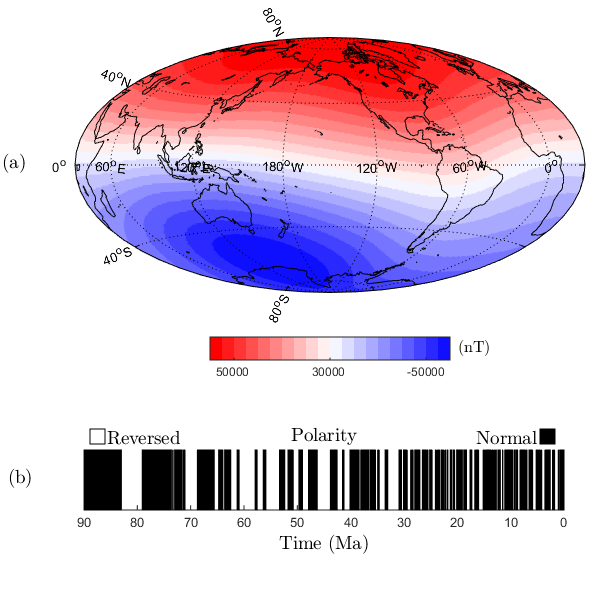
\includegraphics[scale=0.6]{Earth_Field.png}
\caption{(a) Dipolar magnetic field of the Earth in its normal orientation. (b) Polarity of the field inferred from the geological record over the past 90 Ma \cite[]{Cande1995}.}
\label{fig:Earth_Field}
\end{figure}

Natural Remanent Magnetization $\vec M_{NRM}$ is a permanent magnetization moment preserved in the absence of an inducing field.
The reader is encouraged to refer to \cite{Blakely96} and \cite{Clark99} for a more in-depth explanation of chemical, thermal and biological processes responsible for the remanent component of various rock types.
While the induced component is linearly related to the inducing field, nothing can be assumed about the NRM orientation and it remains challenging to estimate.
If aligned with the inducing field direction, the NRM is indistinguishable from a purely induced response, resulting in an over-estimation of the magnetic susceptibility of rocks.
For large NRM components, perpendicular or anti-parallel to the inducing field, the magnetic response of compact objects may get distorted, potentially resulting in false interpretation about the distribution and geometry of rock units.
Direct geological interpretation of magnetic data that ignores the effect of remanence has long been recognized as problem in mineral exploration.
This brings up an important question:
How can we better recover the location and geometry of magnetized objects without knowledge of the total magnetization direction $\vec M$?

From Gauss's law, the relation between the observed magnetic field and rock magnetization is expressed as:
\begin{equation} \label{b_integral}
	\vec b(r) = \frac{\mu_0}{4\pi} \int_{V} \nabla \nabla \frac{1}{ r} \cdot \vec M \; dV\;,
\end{equation}
where $\vec b$ is the magnetic field (T) as measured at some distance $ r$ from a magnetic anomaly with magnetization per unit volume $\vec M$ (A/m).
Since $\vec b$ is usually small, it is commonly measured in units of nano-Tesla (nT).
The majority of magnetic data consist of Total Magnetic Intensity (TMI) measurements which can be written as:
\begin{equation}
	b^{TMI} = |\vec B_0 + \vec B_A| \;,
\end{equation}
where we measure the magnitude of the field rather than the individual components.
In most cases we are only interested in the anomalous local fields.
Under the assumption that $|\vec B_A| \ll |\vec B_0|$, the anomalous field is approximated to be parallel with the direction of the inducing field $\hat B_0$.
The Total Magnetic field Anomaly (TMA) is given by:
\begin{equation}
\begin{split}
	b^{TMA} &= |\vec B_0 + \vec B_A| - |\vec B_0| \\
	&\simeq  \vec B_A \cdot \hat B_0 \;.
\end{split}
\end{equation}
Figure~\ref{fig:Magnetization} gives an example of TMA data measured on a plane above a magnetized sphere.
The main challenge in interpreting magnetic data is to characterize the magnetic sources when nothing is known about the location and magnetic properties ($\kappa,\;\vec M$) of buried objects.
Accurately imaging the location and geometry of magnetic objects is a core problem in exploration geophysics.


\begin{figure}[h!]
\centering
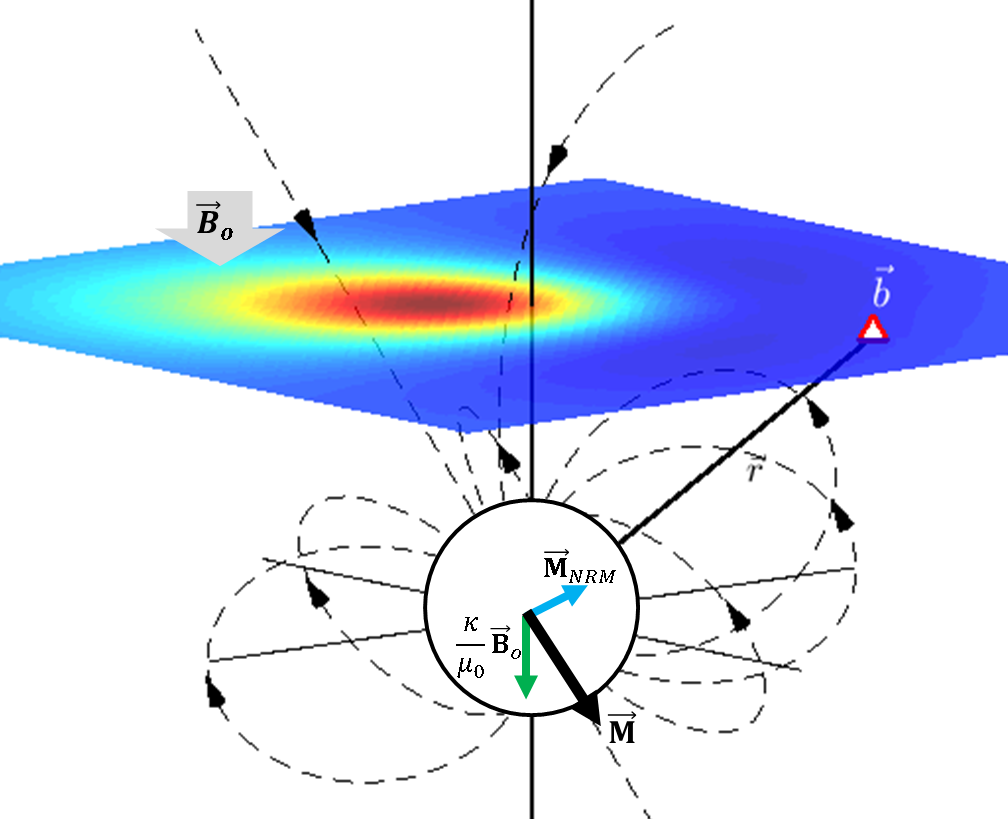
\includegraphics[scale=0.55]{Magnetization_EDT.png}
\caption{Magnetic field data $\vec b$ observed on a plane over a magnetized sphere located at the origin. The orientation and magnitude of magnetization of the sphere is function of the magnetic susceptibility $\kappa$, the inducing field $\vec B_0$ and remanent components $\vec M_{NRM}$, neglecting self-demagnetization effects. }
\label{fig:Magnetization}
\end{figure}

Early geophysical studies relied primarily on filtering techniques to infer geological structures and identify potential targets \cite[]{Cowan2000}.
In order to reduce the complexity of the problem, the magnetization direction is in most cases assumed to be purely induced along $\vec B_0$, neglecting self-demagnetization and remanence effects.
Inversion codes, such as the UBC-MAG3D from \cite{LiOldenburg1996}, also rely on this assumption.
While the induced component may dominate in most cases, recent petrophysical studies seem to indicate that the effect of remanent magnetization may be more important than previously thought \cite[]{Enkin2014}.
This is especially true for specific types of mineral deposits such as Banded Iron-Formations (BIF) and diamondiferous kimberlite \cite[]{Dransfield2003, LiShearer10}
Strong remanent magnetic components can hinder the interpretation of magnetic data thus leading to false drilling targets.

\section{Magnetic methods}
Several studies have been dedicated to the inversion of magnetic data in the presence of remanence.
As summarized by \cite{Li2012}, the proposed inverse methods can be divided into three categories.
The first category estimates the magnetization direction from the data in a pre-processing step.
Strategies such as the Helbig's method \cite[]{Phillips03} and the cross-correlation \cite[]{DannemillerLi06} are used upstream of standard inversion codes.
Adapted from the 2-D analytical signal of \cite{Nabighian72}, \cite{Roest92} estimate the orientation of remanence in 3-D.
In most cases, data are transformed to the wavenumber domain in order to extract magnetic field components.
These methods are simple and robust for simple and isolated anomalies, but become impractical when the data are acquired over rough terrain or complicated geology.

The second category deals with magnetic data that are weakly dependent on the orientation of magnetization.
It has been shown that magnetic amplitude data are weakly dependent on the magnetization direction in 3-D \cite[]{Nabighian72}.
Magnetic amplitude data are simply calculated as:
\begin{equation}
|\vec b| = {( b_x^2 + b_x^2 + b_x^2 )}^{1/2}\;,
\end{equation}
where $b_x$, $b_y$ and $b_z$ are the three components of the anomalous magnetic field.
Inverting magnetic amplitude data can provide a robust estimate for the location of magnetized bodies
as shown by \cite{Shearer05}. Magnetic amplitude data are successfully inverted over a kimberlite deposit, recovering the true location of kimberlite pipes and associated magnetic dykes.
Because most magnetic surveys only record TMI data, the three components of the field must be derived in post-processing.
Two strategies have been proposed in the literature to extract magnetic field components.
The first relies on the fact that magnetic data are potential field data, hence knowledge of any component of the field on an infinite plane above the source is sufficient to calculate the remaining components. 
Data are interpolated onto a uniform grid, which is then used to calculate the components of the field using Fourier transform techniques.
This may be a problem however for airborne surveys over steep topography or acquired at low latitude.
Alternatively, the equivalent-source method has been proposed by \cite{Li2010} to alleviate those constraints.
Taking advantage of the non-uniqueness of potential field data, TMA data are inverted for a layer of magnetic sources then used to forward model three-component magnetic data.


The third method directly solves for the orientation of magnetization without making any assumptions about the location or geometry of causative bodies.
In the Magnetic Vector Inversion (MVI) proposed by \cite{Lelievre2009}, the magnetization vector is decomposed in its induced and orthogonal components.
The MVI is closely related to the method proposed by \cite{Kubota2005}, and later borrowed by \cite{Ellis2012}.
This method results in a large under-determined inverse problem, with roughly three times the number of free-variables over conventional susceptibility inversion codes.
Recovered magnetization models are generally smooth and become overly complicated for direct geological interpretation.
As pointed out by \cite{PhDLelievre09}, any \emph{a priori} information from surface or borehole measurements may greatly reduce the non-uniqueness of the problem.
Unfortunately this kind of information is rarely available in greenfield settings or is only available in sparse samples.

Building upon the work of \cite{Shearer05}, \cite{Liu2015} propose a hybrid three-step process to invert for the location, orientation and magnetic susceptibility distribution in 2-D.
In the first step, the location of magnetic material is inverted from amplitude data.
Next, the orientation of magnetization is found via a correlation method.
The orientation of magnetization is then used in a standard inversion code to recover a susceptibility model.
The combined method greatly reduces ambiguity about the location and orientation of isolated targets, but becomes challenging over multiple anomalies with variable magnetization directions.
The same synthetic model was applied to the MVI method, resulting in a poor recovery for the location and intensity of magnetization.
This result is surprising considering the satisfactory solution obtained in previous studies \cite[]{Ellis2012, Lelievre2009}.
The combined approach of \cite{Liu2015} is interesting however, as it links together complementary algorithms.

\section{Thesis outline}
Following the same line of thought as \cite{Liu2015}, I propose a Cooperative Magnetic Inversion (CMI) algorithm that directly incorporates the amplitude inversion of \cite{Shearer05} into the MVI algorithm of \cite{Lelievre2009}.
Magnetic field amplitude data are computed from the Equivalent Source technique proposed by \cite{Li2010}, removing the need to grid the data.
Moreover, I introduce a Scaled Iterative Re-weighted Least Squares (S-IRLS) regularization method to recover blocky and sparse solutions.
My thesis is divided into the following chapters:

In Chapter~\ref{ch:Chap2_Forward} and \ref{ch:Chap3_Inverse}, I provide further details about rock magnetism and review the theory related to inverse problems in the context of exploration geophysics. I revisit three inversion codes from the literature: the magnetic susceptibility inversion from \cite[]{LiOldenburg1996}, the magnetic amplitude inversion from \cite{Shearer05}, and the Magnetic Vector Inversion (MVI) from \cite[]{PhDLelievre09}.
Each of these codes are tested on a synthetic example with complicated magnetization distribution.
I also review the equivalent-source method from \cite{Li2010}.

In Chapter~\ref{ch:Chap4_Mixed_Lpnorm_Regularization}, I introduce a mixed $l_p$-norm regularization function for the recovery of compact and sparse solutions, increasing the flexibility of current inversion codes.
The method uses a Scaled Iterative Re-weighted Least Squares (S-IRLS) formulation to approximate any $l_p$-norm penalties on the interval $0 \le p \le 2$.
Sparse constraints are applied on both the model and model gradients independently.
The mixed-norm regularization is implemented on the magnetic problem, and tested on an airborne magnetic dataset from the Tli Kwi Cho kimberlite complex, Northwest Territories.

In Chapter~\ref{ch:Chap5_Cooperative_Mag_Inversion_CMI}, I formulate a Cooperative Magnetic Inversion (CMI) method, combining the inversion codes presented in Chapter~\ref{ch:Chap3_Inverse} and \ref{ch:Chap4_Mixed_Lpnorm_Regularization}.
The algorithm is tested on the same synthetic example for comparison.

Finally in Chapter~\ref{ch:Chap6_Case_Study}, I apply the CMI algorithm to a large aeromagnetic data set over the Ekati Property, Northwest Territories.
I design a tiled inversion scheme to automate the inversion process and to reduce the computational cost.
Individual models are then merged back onto a global mesh for analysis.
A bulk estimate of magnetization direction is compared to values published in the literature.
The polarities of magnetization over 11 pipes are compared to the estimated age of emplacement.
The analysis is extended to various dyke swarms, providing regional geologic information.

The work presented in this thesis is significant for two reasons.
First, the mixed-norm regularization function introduced in Chapter~\ref{ch:Chap4_Mixed_Lpnorm_Regularization} can considerably improve the flexibility of inversion algorithms, not limited to potential field problems.
The S-IRLS method allows for a combination of sparse norms on the model and model gradients independently, granting access to a wider range of solutions than previously offered by globally convex functions.
%Future research will focus on the implementation of the S-IRLS on other geophysical inverse problems such as for gravity and electromagnetic data.

Secondly, it is the first time that both the amplitude inversion and MVI algorithms are combined in a cooperative inversion method in 3-D.
Structural information gained by the amplitude inversion is used directly to constrain the MVI algorithm, reducing the non-uniqueness of the solution.
From a practical standpoint, it is an automated process that streamlines the inversion workflow.
This, in turn, can reduce the overall time required to process magnetic data and promote the expansion of inversion methods in mineral exploration.
%Future research will focus on the implementation of a non-linear spherical formulation for the MVI, improving the flexibility of the algorithm.

\endinput


%% The following is a directive for TeXShop to indicate the main file
%%!TEX root = Thesis_Driver.tex
\graphicspath{{./../../Figures/}}
\chapter{Forward modeling of potential field data}
\label{Chapter2}
My goal is to characterize the sub-surface in terms of density and magnetization. In Chapter~\ref{Chapter1}, I have introduced the basic physics describing the relation between density and magnetization and their respective anomalous fields in integral form. In this chapter, I provide numerical details about the transformation from the continuous space to a discrete linear system of equations. I also provide efficiency improvements over conventional implementations for the processing of large scale data sets.

\section{Discrete systems}
The usual strategy is to represent the continuous Earth in terms of unit elements each contributing to the total response observed at a given position in space.
For the gravity problem, the integral in \eqref{g_integral} can be evaluated analytically over a discrete prism with uniform density $\rho$. As derived by \cite{Nagy66}, the integration gives rise to a linear system:
\begin{equation} \mathbf{g} = \begin{bmatrix} T_{x} \\ T_{y} \\ T_{z} \end{bmatrix} \; \rho \;, \label{gfield} \end{equation}
where $\mathbf{T}$ relates the cell-centered density value to the observed gravity field $\mathbf{g}$ at some location $P(x_P, y_P, z_P)$:
\begin{equation}
\begin{split}
T_{x} &= -G \bigg( \arctan \frac{dy\;dz}{r\:dx} + \log \left[\; dz + r\;\right] + \log \left[\; dy + r\;\right] \bigg) \bigg|_{x_L}^{x_U} \bigg|_{y_L}^{y_U} \bigg|_{z_L}^{z_U}\\
T_{y} &= -G \bigg( \arctan \frac{dx\;dz}{r\:dy} + \log \left[\; dz + r\;\right] + \log \left[\; dx + r\;\right] \bigg) \bigg|_{x_L}^{x_U} \bigg|_{y_L}^{y_U} \bigg|_{z_L}^{z_U}\\
T_{z} &= -G \bigg( \arctan \frac{dy\;dy}{r\:dz} + \log \left[\; dy + r\;\right] + \log \left[\; dy + r\;\right] \bigg) \bigg|_{x_L}^{x_U} \bigg|_{y_L}^{y_U} \bigg|_{z_L}^{z_U}\\
r &= (dx^2 + dy^2 + dz^2)^{1/2} \\
dx &= (x_P - x), \; dy = (y_P - y),\; dz = (z_P - z)\\
\end{split}
\label{Tmatrix}
\end{equation}
and $G$ is Newton's gravitational constant.
Parameters needed to define the position and shape of a unit cell are presented in Figure~\ref{UnitCube}. Only the lower southwest $L(x_L,y_L,z_L)$ and upper northeast $U(x_U,y_U,z_U)$ corner coordinates are needed to define the relative distance $\mathbf{r} (dx,\:dy,\:dz)$ between the observation point and the nodal limits. In this research I use right-handed Cartesian coordinate system such that the $\hat x$, $\hat y$ and $\hat z$ coordinate axes point along the east, north and vertical (up) direction respectively.
\begin{figure}[h!]
\centering{
\includegraphics[width=0.55\columnwidth]{PF_UnitCube.png}}
\caption{Parameters describing the spatial relationship between an observation point $P$ and a rectangular prism $C$.}
\label{UnitCube}
\end{figure}

For most gravity field experiments only the vertical component of field $g_z$ is measured, such that \eqref{gfield} reduces to
\begin{equation}
\begin{split}
g_z =\;& {T}_z \;{\rho} \\
\end{split}\label{g_discrete}
\end{equation}
Equation~\eqref{g_discrete} defines the gravity response of a single rectangular prism as observed at a single position in space. I can augment equation \eqref{g_discrete} to describe a gravity experiment conducted over a large volume of earth and at many observation stations
\begin{equation}\label{g_discrete_large}
	\mathbf{g}^{pre} = \mathbf{G} \boldsymbol{\rho}
\end{equation}
such that the linear forward operator $\mathbf{G}\in \mathbb{R}^{N\times M}$ maps the contribution of $M$ number of prisms ($\boldsymbol{\rho} \in \mathbb{R}^M$), each contributing to the response measured over $N$ observation locations ($\mathbf{g}^{pre} \in \mathbb{R}^{N}$).
There are many ways to organize the cells making up this discrete model.
In all the work presented in this thesis, I use an Octree-based discretization.
More details regarding this choice of parameterization are provided in the following section.

Similarly for the magnetic response, the integral equation in \eqref{b_integral} can be evaluated analytically for a single prism \cite[]{Sharma66}. This gives rise to a linear system of the form
\begin{equation}\label{b_discrete}
\begin{split}
	\mathbf{b} = \mathbf{T} \mathbf{m} \;,
\end{split}
\end{equation}
where $\mathbf{T}$ is a dense 3-by-3 symmetric matrix describing the linear relation between a prism with magnetization $\mathbf{m} = [M_x,\;M_y,\;M_z]^T$ to the components of the field $\mathbf{b} = [b_x,\;b_y,\;b_z]^T$.
\begin{equation}
\begin{split}
\mathbf{T} & = \frac{\mu_0}{4\pi} \begin{bmatrix} T_{xx}& T_{xy}& T_{xz} \\T_{xy} & T_{yy} & T_{yz} \\ T_{xz}&T_{yz} & T_{zz} \end{bmatrix} \\
\end{split}
\label{Tmatrix}
\end{equation}
where $\mu_0$ is the magnetic permeability of free-space. It is important to note that the tensor $\mathbf{T}$ is a symmetric matrix with zero trace. Therefore only five of the nine tensor components need to be calculated.
\begin{equation}
\begin{split}
T_{xx} &= -\arctan \frac{dx\;dy}{{dx}^2 + r\:dz + {dz}^2} \bigg|_{x_L}^{x_U} \bigg|_{y_L}^{y_U} \bigg|_{z_L}^{z_U} \\
T_{yy} &= -\arctan \frac{dx\;dy}{{dy}^2 + r\:dz + {dz}^2} \bigg|_{x_L}^{x_U} \bigg|_{y_L}^{y_U} \bigg|_{z_L}^{z_U} \\
T_{xy} &= \log \left[\; dz + r\;\right] \bigg|_{x_L}^{x_U} \bigg|_{y_L}^{y_U} \bigg|_{z_L}^{z_U}\\
T_{xz} &= \log \left[\; dy + r\;\right] \bigg|_{x_L}^{x_U} \bigg|_{y_L}^{y_U} \bigg|_{z_L}^{z_U}\\
T_{yz} &= \log \left[\; dx + r\;\right] \bigg|_{x_L}^{x_U} \bigg|_{y_L}^{y_U} \bigg|_{z_L}^{z_U}\\
%T_{zz} &= -\arctan \frac{dx\;dy}{r\:dz} \bigg|_{L_x}^{U_x} \bigg|_{L_y}^{U_y} \bigg|_{L_z}^{U_z} \\
\end{split}
\end{equation}


For most geophysical applications, we do not measure the vector field $\vec b$, but rather the Total Magnetic Intensity (TMI) of the field that includes both the geomagnetic and secondary fields. Since we are only interested in the anomalous response from rocks, the approximation is generally made that
\begin{equation}\label{TMIprojection}
{b}^{TMA} = \vec{b} \cdot {{\hat H_0}} - \mu_0\|\vec{H}_0\|;
\end{equation}
such that the Total Magnetic Anomaly $b^{TMA}$ is assumed to be small and parallel to Earth's field $\vec{H}_0$.
The simulated magnetic datum in \eqref{b_discrete} simplifies to
\begin{equation}
\begin{split}
{b}^{pre} =\; \left[ \mathbf{ {\hat H}}_0^\top \cdot \mathbf{T}\right]\;\mathbf{m}
\end{split}
\end{equation}
Just as for the gravity experiments, this system can be augmented for $M$ number of prisms ($\mathbf{m} \in \mathbb{R}^{3M}$) and $N$ observation locations ($\mathbf{b}^{pre} \in \mathbb{R}^{N}$)
\begin{equation}\label{magLinearOpt}
\mathbf{b}^{pre} =\; \mathbf{F} \;\mathbf{m}
\end{equation}
such that $\mathbf{F}\in \mathbb{R}^{N\times 3M}$. This linear system has three times the number of parameters compared to the gravity problem as magnetization is a vector property.
As part of my contribution to the open-source community, both the gravity and magnetic kernels have been added to the \texttt{SimPEG.PF} library.

\subsection{Choice of discretization}
I have so far established the linear equations \eqref{g_discrete_large} and \eqref{magLinearOpt} that map the gravity and magnetic response for a collection of rectangular prisms making up a discrete Earth. I have yet to define how these cells are organized in a 3D space. This decision will directly affect the size of the forward (and later inverse) calculations as the size of the linear operators scale linearly with respect $M$. Approximating the Earth more efficiently will allow me to process large data sets.

The usual strategy is to define a core region of interest with a fine discretization and surround it by coarser cells (padding) to absorb regional signals that may be present in the data.
Two options are available to organize rectangular prisms.
The simplest implementation uses a regular grid, or tensor mesh shown in Figure~\ref{MeshType}(a). Each unit element shares a face with 6 neighbours. Changes in cell size propagate throughout the domain along the orthogonal direction. The use of tensor meshes has dominated the inversion literature due to the ease of storing and viewing uniformly gridded models.
\begin{figure}[h!]
{\centering
\includegraphics[width=\columnwidth]{MeshType.png}}
\caption{Simple representation of (a) tensor and (b) Octree meshes for the organization of rectangular prisms within a core domain (red) and padding region over a square domain 4 x 4 m in width. The Tensor mesh can fill the space with 64 cells, compared to only 40 cells with the Octree mesh.}
\label{MeshType}
\end{figure}

In an Octree mesh, unit cells are organized in a hierarchical structure as shown in Figure~\ref{MeshType}(b). The resolution of the grid is increased by dividing a parent cell into 8 children (or 4 in 2D). This type of discretization offers the most flexibility for increasing the resolution of the mesh in a specific region without affecting the resolution of boundary cells.
The main challenge is in generating a mesh that honours the geometry of the problem in terms of data location, topography and geological contacts.
Over the course of my research, I contributed to the open-source community with a suite of refinement functions to facilitate the creation process of Octree meshes.
As part of the \texttt{SimPEG.discretize} library, I implemented the following three strategies:
\begin{itemize}
\item Box refinement includes all cells intersected by a rectangular box containing the input points.
\item Radial refinement is performed inside spheres centered on each input points. The radial distance is determined by the user.
\item Surface refinement is defined by a continuous Delaunay triangulation of the input points \cite[]{Barber1996}. The Octree refinement is determined based on the vertical distance between cell centers and the nearest triangle. 
\end{itemize}
Figure~\ref{Refinements} compares the three refinement methods for the discretization of points (red) placed on a  Gaussian surface. The \texttt{box} refinement is the simplest but also the least efficient strategy as it yields a uniform grid similar to the Tensor discretization. For the \texttt{radial} refinement, I end up with a small number of cells concentrated around the input points. It is an optimal refinement for scattered observation points. The \texttt{surface} is well suited to describe continuous features such as topography and geological contacts. It gives, in this case, the most accurate representation of the Gaussian surface.
\begin{figure}[h!]
{\centering
\includegraphics[width=\columnwidth]{Refinements.png}}
\caption{Three refinement strategies used to discretize a Gaussian curve defined by scattered points (red): (a) \texttt{box}, (b) \texttt{radial} and (c) \texttt{surface} refinement strategy from the \texttt{SimPEG.discretize} library. Cells are coloured by their corresponding Octree level.}
\label{Refinements}
\end{figure}

\subsubsection{Forward simulation test}
I demonstrate the benefit of an Octree discretization by forward modelling the response of a 1 m sphere shown in Figure~ \ref{Discretization}. I want to compare the numerical cost to perform forward simulations using the standard Tensor discretization and an Octree mesh with \texttt{surface} refinement.
Octree refinement uses scatter points placed on the outer surface of the sphere. Using equation \eqref{b_discrete}, I calculate the magnetic response over an 11-by-11 grid of observations placed 1 m above the anomaly. I repeat the forward simulation over a range of cell sizes. Only cells inside the sphere are considered.
The forward calculations are compared to the analytical vertical response ($b_z^{ana}$) for a vertical magnetization:
\begin{equation}
b_z^{ana} = \frac{\mu_0}{4\pi}\left[ -\frac{{\bf M}}{r^{\,3}} + \frac{3\,({\bf M}\cdot{\bf r})\,{\bf r}}{r^{\,5}} \right] \cdot \hat z
\end{equation}
where $\mathbf{M}=[0\:\hat x\;, 0\:\hat y,\; 1\:\hat z]$ and $\mathbf{r}$ defines the vector between the center of the sphere and the observation location.
Table~\ref{AnalyticSphere} summarizes the forward calculations in terms of total number of cells, run time and data residual between the simulation and the analytic solution.
\begin{equation}\label{dataResidual}
\phi_d = \sum_{i=1}^{121} (b_{i} - b_{i}^{ana})^2
\end{equation}
All calculations were performed on a single thread 2.4 GHz Intel processor.
\begin{figure}[h!]
{\centering
\includegraphics[width=\columnwidth]{Discretization.png}}
\caption{(a) Discretization of a sphere defined by discrete points (red) using the conventional Tensor mesh with a core region and padding cells. Octree meshes refined by (b) \texttt{box}, (c) \texttt{radial} and (d) \texttt{surface} methods from the \texttt{SimPEG.discretize} library. }
\label{Discretization}
\end{figure}

For the Tensor mesh, a reduction in core cell size increases the total number of cells by a factor 8. For the same reduction in cell size using the surface refinement increases the number of cells by a factor 4. This is anticipated as only cells at the surface of the sphere decrease in size compared to a full volume refinement in the Tensor mesh. Both discretizations can reproduce the analytical response with roughly the same accuracy. Including padding cells to this problem would further increase the efficiency gap between the two discretization methods as the Octree mesh can rapidly increase the cell size with little influence from the discretization in the core region.
\begin{table}\centering
\begin{tabular}{|c|c|c|c||c|c|c|}\hline
& \multicolumn{3}{c}{Tensor} \vline \vline & \multicolumn{3}{c}{Octree (Surface)}\vline \\ \hline
Cell size (m) & \# Cells & Time (s) & $\phi_d$ & \# Cells & Time (s) & $\phi_d$ \\ \hline
1.00e-01 & 544 & 1.8e-01 & 4.2e+02 & 496 & 1.6e-01 & 7.7e+02 \\
5.00e-02 & 4196 & 9.6e-01 & 4.7e+01 & 2516 & 5.1e-01 & 7.1e+01 \\
2.50e-02 & 33478 & 6.5e+00 & 4.2e+00 & 10836 & 2.1e+00 & 5.2e+00 \\
1.25e-02 & 268080 & 6.5e+01 & 2.0e+00 & 47276 & 1.0e+01 & 2.7e+00 \\
\hline
\end{tabular}
\caption{Summary table for the forward modeling of a magnetized sphere using a Tensor and Octree discretization}
\label{AnalyticSphere}
\end{table}


\section{Large scale problems}\label{MeshDecoupling}
The amount of memory needed to store the dense linear operators for gravity and magnetics is a limiting factor for the simulation of potential field data with the integral formulation. As prescribed in \eqref{magLinearOpt}, the size of the problem is linearly scaled by the number of model parameters $M$ and the number of the data $N$. For moderate size problems encountered in exploration geophysics ($M\approx 10^6$, $N\approx10^4$) the memory requirement to store a dense $M\times N$ matrix can exceed hundreds of gigabytes. While modern supercomputers can handle problems of this size, it is still out of reach for common desktop computers.

A number of strategies have been proposed in the past to reduce the size of the problem. Compression methods, either in the Fourier \cite[]{Pilkington97} or wavelet domain \cite[]{LiOldenburg03}, have proven successful in reducing the size of the forward operators. On the downside, compression methods are prone to introducing modelling artifacts, which can be hard to differentiate from true anomalies. This is especially an issue for the magnetic vector inversion explored in Chapter~\ref{Chapter3}.

Another group of methods takes advantage of the rapid decay of geophysical signals to reduce the size of individual forward simulations. The assumption is made that model parameters in the far-field of measurements contribute little to the total response and can, therefore, be approximated with fewer parameters. In this regard, the concept is loosely related to the Fast Multipole Method \cite[]{Engheta1992}. This is especially valid for airborne EM experiments where cells beyond roughly 10 times the flight height of airborne EM systems have a negligible impact on the measured response \cite[]{Reid2006}. In its simplest implementation, \cite{Cox2010} define a footprint approach such that model parameters outside a pre-defined tolerance are simply ignored.

More recently, \cite{Yang2014} introduced a mesh decoupling approach. Local meshes are designed based on the source location and decay rate of the geophysical signal. Cell-centered conductivity values are homogenized using volumetric-weighted averaging. Similarly, \cite{Haber2014} designed a nested Octree mesh strategy. The core region of local meshes is co-located with cells in the global mesh and cover the same lateral extent. Physical property values are homogenized from small cells in the global mesh to larger (or equal) cells in the local meshes. This strategy assures that far-field features can still contribute to the total response. The accuracy of individual forward simulations depends primarily on the interpolation scheme used to transfer physical properties from the global to the local meshes.

In this research, I employ the methodology of \cite{Haber2014}. I want to divide the full data set into subsets (or tiles), each associated with a local mesh. Physical property values are transferred to local meshes using a volumetric weighted average. In order to further minimize the memory footprint of the simulation, I make use of the parallel \texttt{Dask} package \cite[]{dask2016}. The library was designed by the data science community for out-of-core processing of large datasets \cite[]{Scipy2015}. The \texttt{zarr} file format allows the storage of dense arrays on a solid-state drive (SSD) in compressed memory chunks. Out-of-core storage is appealing as it reduces the amount of Random-Access Memory (RAM) needed to store the large forward operators. Read and write operations are done in parallel. The runtime depends largely on the hardware used in terms of processor speed, number of processors and communication speed between the workers and the solid-state memory. The size of individual memory chunks can be adjusted to optimize the processing speed depending on the resources available.

In the case of potential field data, the source of geophysical signals can span a broad range of wavelengths, from tens of meters (local) to hundreds of kilometres (regional). The memory footprint of a problem can be reduced considerably if we manage to approximate far-field features with fewer cells. In the most extreme case, each observation point could have its own local mesh.
Choosing the number of tiles becomes a trade-off between accurately capture the heterogeneity of the model for forward modeling while minimizing traffic between the parallel workers and the SSD memory.

\subsection{Numerical test}
I investigate this trade-off between accuracy and efficiency with a numerical example.
I create a synthetic gravity model shown in Figure~\ref{Tiled_Test_model}. The model contains both short wavelength information from a small block anomaly and long wavelength signal from large domains in the north and southeast quadrants. From equation \eqref{g_discrete_large}, I compute gravity data on $21 \times 21$ grid placed 1 m above a flat topography.
Forward simulation of the global model required 4.3 Mb of memory and was performed in parallel in 6.7 s with 4 processors (2.4 GHz). It is a relatively small example compared to industry standards, but similar trends are to be expected on larger scale problems.
\begin{figure}[h!]
{\centering
\includegraphics[width=\columnwidth]{Tiled_Test_model.png}}
\caption{(a) Horizontal and (b) vertical sections through the synthetic density model used to test the mesh decoupling strategy. (c) The simulated data contain short and long wavelength information.}
\label{Tiled_Test_model}
\end{figure}

I will assess the trade-off between efficiency and numerical accuracy by performing a series of five forward simulations using a range of tiling patterns. I break up the dataset into 2, 4, 9, 12 and 16 square tiles.
For each tiling experiment, I calculate the total memory footprint (Gb) and the computation time (s) to perform the forward simulations. I also compute the data residual between the global simulation (single mesh) and the tiled simulation using the $\ell_2$-norm measure in equation \eqref{dataResidual}.
\begin{figure}[h!]
{\centering
\includegraphics[width=\columnwidth]{Tiled_Dask.png}}
\caption{Example of mesh decoupling of the forward problem into nested Octree tiles. (Middle) Local meshes are generated for a pre-defined number of tiles nested inside the global domain. (Bottom) The forward modelling operator for each tile is stored in compressed \texttt{Zarr} file format on solid-state memory. Memory chunks (grey) are accessed in parallel by the \texttt{Dask} library to perform the forward calculations.}
\label{Tiled_Dask}
\end{figure}

As seen in Figure~\ref{Tiled_Test_Size}, the memory needed to perform the forward calculations rapidly decreases but eventually levels-off as the number of tiles increases. This is expected as local meshes necessitate a minimum number of cells to fill out the global domain and a minimum number of small padding cells near the edge of the tiles to reduce interpolation artifacts. The reduction in problem size is inversely correlated with an increase in computational time as communication between the workers and the SSD memory becomes a bottleneck.
\begin{figure}[h!]
{\centering
\includegraphics[width=\columnwidth]{Tiled_Test_Size.png}}
\caption{Trade-off curves between the size of the forward problem (blue) and data residual (red) over a range of number of tiles. The total size of the problem is calculated based on the sum of cells in all the local meshes times the number of data. The optimal number of tiles would be at the point of intersection where both the cost of forward calculations and the data residual change significantly.}
\label{Tiled_Test_Size}
\end{figure}

I also note an increase in data residual as a function of tile size.
Figure~\ref{Tiled_Residual} compares the simulated data from the global mesh (single tile) to the combined forward simulation calculated with 12 tiles (last experiment). From the residual map, it is possible to distinguish short wavelength discrepancies between adjacent forward simulations (tiles). These residuals are primarily due to the homogenization of anomalies near the edges of tiles, which in turn is a function of the wavelength information contained in the data. As a first pass, I establish experimentally the appropriate padding distance based on the estimated data uncertainties, such that the maximum residual falls below the experimental error. For this experiment, the meshing artifacts are at most $2\%$ of the data amplitude (or 0.004 mGal), which I achieved with a minimum padding distance of 4 cells per Octree level. Determining an optimal padding distance as a function of the geophysical signal would warrant further research. 
\begin{figure}[h!]
{\centering
\includegraphics[width=\columnwidth]{Forward_Tiles.png}}
\caption{Simulated gravity data calculated from (a) the global model and (b) the 12 forward tiled calculations. (c) Data residuals show short wavelength discrepancies between adjacent tiles due to interpolation effects.}
\label{Tiled_Residual}
\end{figure}


\endinput


%% The following is a directive for TeXShop to indicate the main file
%%!TEX root = Thesis_Driver.tex
\graphicspath{{./../../Figures/}}
\chapter{Inverse Problem}
\label{Chapter3}
In Chapter~\ref{Chapter2}, I defined the linear equations relating density and magnetization to gravity and magnetic data. I now review the theory needed to solve the inverse problem, such that I can recover a 3D representation of the subsurface from the observed data.
A key issue related to the inverse problem is that there is an infinite number of
possible models that can satisfy the data. Field measurements are generally acquired from the surface resulting in the inverse problem to be ill-posed. The presence of experimental noise further complicates the problem.
To circumvent these issues, the inversion is often formulated as an optimization problem of form
\begin{equation}
\begin{split}\label{GenMinProb}
\underset{\mathbf{m}}{\text{min}}\; \phi(m) & = \; \phi_d + \beta \phi_m \\
\text{subject to} \; \phi_d & \leq \phi_d^* \; .
\end{split}
\end{equation}
where $\phi_d$ is the misfit function
\begin{equation}\label{eq:misfit}
\phi_d =\sum_{i=1}^{N}\left(\frac{d_i^{pred} - {d}_i^{obs}}{\sigma_i}\right)^2 \;,
\end{equation}
that measures the residuals between the observed and predicted data $\mathbf{d}^{pre}$, normalized by the estimated data uncertainties $\boldsymbol{\sigma}$.

The regularization function $\phi_m$, or model objective function, serves as a vehicle to introduce \emph{a priori} information in the inversion.
Several regularization strategies have been developed over the last decades such that the solution remains geologically plausible.
I focus on the generic $\ell_p$-norm regularization of the form
\begin{equation}
\begin{split}\label{intSmall}
\phi_m &= \sum_{r=s,x,y,z} \alpha_r \int_V w(m) |f_r (m)|^{p_j} \;dV\;. \\
\end{split}
\end{equation}
The functions $f_r$ can take many forms but most often have been
\begin{equation}
\begin{split}\label{fj}
f_s= m-m^{ref},\;f_x= \frac{d m}{dx},\; f_y= \frac{d m}{dy},\;f_z= \frac{d m}{dz}\;.
\end{split}
\end{equation}
Thus $f_s(m)$ measures the deviation from a reference model $m^{ref}$ and $f_x(m)$, $f_y(m)$ and $f_z(m)$ measure the roughness of the model $m$ along orthogonal directions in 3D.  
This optimization problem has multiple terms scaled by hyper-parameters. The first parameter is $\beta$ which controls the balance between misfit and regularization. It is assumed that a value can be found such that the target misfit is reached.
The $\alpha$'s are constants that control the relative influence of the different regularization functions. A larger $\alpha$-value increases the focus of the optimization on the corresponding penalty function.
User-defined weights $w(m)$ are used to incorporate any type of \emph{a priori} information that may be available to guide the solution.
 
Most often the $\ell_2$-norms measure has been used giving rise to a discrete linear system of form
\begin{equation}\label{leastSquaresLin}
\begin{split}
\phi_m &= \alpha_s \phi_s + \alpha_x \phi_x +\alpha_y \phi_y+\alpha_z \phi_z\\
& = \sum_{r=s,x,y,z} \alpha_r \|\mathbf{W}_r \;\mathbf{V}_r \;\mathbf{G}_r \;(\mathbf{m}-\mathbf{m}^{ref})\|_2^2 \;,\\
\end{split}
\end{equation}
where $\phi_s$ measures the deviation of the discrete model $\mathbf{m}$ from a reference model $\mathbf{m}^{ref}$ and $\phi_x$, $\phi_y$ and $\phi_z$ measure the roughness of the model along Cartesian directions. The reference model is sometimes omitted in the roughness terms. The matrices $\mathbf{G}_x,\;\mathbf{G}_y,$ and $\mathbf{G}_z$ are discrete gradient operators. 
For the smallness component, $\mathbf{G}_s$ reduces to the identity matrix. Volumes of integration resulting from the evaluation of \eqref{intSmall} are applied through diagonal matrices such that 
\begin{equation}
\mathbf{V}_s = diag\left[ \mathbf{v}^{1/2}  \right]\;.
\end{equation}
where $\mathbf{v}$ holds the discrete volume elements corresponding to each cell.
For the model derivative terms, the volume of integration is computed over cell interfaces such that
\begin{equation}\label{volumeAve}
\mathbf{V}_x = diag\left[\left( \mathbf{A}_C^{F_x} \mathbf{v}\right)^{1/2}  \right]\;.
\end{equation}
where the matrix $\mathbf{A}_C^{F_x}$ averages the cell-centered volumes to cell faces. Similar averaging is performed along the orthogonal $y$ and $z$-direction. Diagonal matrices $\mathbf{W}_r$ hold user-defined weights. More details about these weights are provided in the following section. 
Lastly, the $\alpha$ parameters control the relative importance given to individual components of the regularization.
What is sometimes sought, at least as a first pass, is that if $\phi_s$, $\phi_x$, $\phi_y$, $\phi_z$ have about the same numerical value then they are contributing equally. Dimensional analysis shows that for a uniform discretization $h$:
\begin{equation}\label{lengthScale}
\frac{[\phi_x] }{ [\phi_s]} = {[h]}^{-2}\;.
\end{equation}
The common approach is to set $\alpha_s$ accordingly in order to scale the components of the regularization function.

The usual strategy to solve \eqref{GenMinProb} is through a gradient descent algorithm, such as a Gauss-Newton approach, where we attempt to find a solution that has zero gradients
\begin{equation}\label{gradPhi}
\mathbf{g} = \nabla_m \phi(\mathbf{m}) = \nabla_m \phi_d + \beta \bigg[ \alpha_s \nabla_m \phi_s + \alpha_x \nabla_m \phi_x + \alpha_y \nabla_m \phi_y + \alpha_z \nabla_m \phi_z \bigg] = \mathbf{0} \;.
\end{equation}
where $\nabla_m$ stands for the partial derivatives of the function with respect to the discrete parameterization $\mathbf{m}$.
A solution to \eqref{gradPhi} can readily be calculated by gradient descent methods \cite[]{HestenesStiefel1952, NocedalWright99}.

A large number of studies have made use of this formulation to incorporate a variety of \emph{a priori} information: physical property data from rock and core samples \cite[]{LelievreOldenburgWilliams09}, structural knowledge \cite[]{LiDWO2000, PhDLelievre09} and advanced 3D geological modeling (\cite[]{Phillips1996, Williams08, Bosh2001, Fullagar2008}.
Although successful in identifying imaging anomalies at depth, penalty functions that rely on $\ell_2$-norm measures have a limited range of possible outcomes. The models tend to be smooth and difficult to interpret in relation to known geological domains with discrete boundaries. Moreover, substantial modelling work is generally required by experts to manually refine these constraints in order to test different geological scenarios.

\subsubsection{Sensitivity weighting}
The weighting matrices $\mathbf{W}_r$ introduced in \eqref{leastSquaresLin} can take many forms depending on the type of \emph{a priori} information that may be available. For potential fields problems, a sensitivity weighting function is generally used to counteract the rapid decay of the geophysical signal as a function of distance. In the work of \cite{LiOldenburg1996}, a \emph{distance weighting} approximation is employed and fixed at the onset.
In this thesis, I resort to an iterative re-weighting strategy based on the sensitivity of a given inverse problem
\begin{equation}\label{Jk}
\mathbf{J} = \frac{\partial \; F[\mathbf{m}]}{\partial \boldsymbol{\mathbf{m}}}\;,
\end{equation}
where $\mathbf{J}$, also referred to as the Jacobian matrix, holds the partial directives of the forward problem $F[\mathbf{m}]$ with respect to $\mathbf{m}$.
Adapted from \cite{Haber1997}, I formulate the sensitivity-based weighting function:
\begin{equation}\label{iter_sens_weight}
\begin{split}
\mathbf{W}_s &= \rm{diag} \left[ {\left[\frac{\mathbf{ w}}{\rm{max}(\mathbf{ w})}\right]}^{1/2}\right]\\
%\mathbf{\hat w}_r &= \frac{\mathbf{ w}_r}{max(\mathbf{ w}_r)}\\
w_{j} &= {\left[\sum_{i=1}^{N}{J_{ij}}^2 + \delta \right]}^{1/2} \Big/ v_j\;,
\end{split}
\end{equation}
where $\mathbf{w}$ measures the sum square of the columns of the Jacobian, normalized by the cell volumes. The constant $\delta$ is a small value (near machine precision) added to avoid singularity. The weights are normalized by the maximum value such that the range of weights are bounded between [0, 1]. 
The same sensitivity weights can also be applied to the model derivative terms using a cell averaging operation such that
\begin{equation}\label{sensWAve}
\mathbf{W}_x = diag\left[\left( \mathbf{A}_C^{F_x} \left[\frac{\mathbf{ w}}{\rm{max}(\mathbf{ w})}\right]\right)^{1/2}  \right]\;,
\end{equation}
similar to the averaging of volumes used in \eqref{volumeAve}. 
This sensitivity weighting strategy is general and adaptable to any inverse problems where the sensitivity matrix can be calculated explicitly.
While the initial purpose of the sensitivity weighting function of \cite{LiOldenburg1996} is to simply counteract the decay of potential fields, I will show numerically in Chapter~\ref{Chapter4} that the iterative re-scaling process can also be beneficial in improving the convergence of gradient methods applied to non-linear inverse problems.


\subsection{Synthetic gravity example}
As an entry point to the inverse problem, I proceed with a simple synthetic gravity example. I define a volume of interest 600 m wide by 300 m deep, over which I place a uniform survey grid of 21 x 21 stations placed 5 m above a flat topography.
The core region directly below the survey grid is discretized at a 5 m resolution as shown in Figure~\ref{GRAV_model}(a)
Within the core region, I build a geophysical target made up of a single dense cube, 25 m in width. I set the density contrast of the prism to 0.2 g/cc in a uniform zero background. From \eqref{g_discrete}, I simulate the vertical gravity field of the block and add random Gaussian noise with $10^{-3}$ mGal standard deviation. Figures~\ref{GRAV_model}(b) and (c) display the simulated data and `noisy' observations $\mathbf{g}_z^{obs}$ used in the inversion. I revisit this example in Chapter~\ref{Chapter4} to demonstrate the inversion process on magnetic data.
\begin{figure}[h!]
{\centering
\includegraphics[width=\columnwidth]{GRAV_Synthetic_True_data_model.png}}
\caption{(a) Vertical section through a 25 m cube with density $\rho$=0.2 g/cc placed in a uniform zero density background. (b) Simulated gravity data responses on a $21 \times 21$ survey grid placed 5 m above the flat topography. (c) Gravity data with random Gaussian noise added, $10^{-3}$ mGal standard deviation.}
\label{GRAV_model}
\end{figure}

From the noisy data I will attempt to recover the block anomaly by the inverse process. The objective function to be minimized takes in this case the form:
\begin{equation}
\begin{split}
\underset{\mathbf{m}}{\text{min}}\; \phi(m) & = \; \|\mathbf{G}\;\boldsymbol{\rho} - \mathbf{d}^{obs}\|_2^2 + \beta \sum_{r=s,x,y,z} \alpha_r \|\mathbf{W}_r \mathbf{V}_r \;\mathbf{G}_r \;\boldsymbol{\rho}\|_2^2 \\
\text{subject to} \; \phi_d & \leq \phi_d^* \;
\end{split}\label{gravLineObjFun}
\end{equation}
where I set $\boldsymbol{\rho}^{ref}=\mathbf{0}$.
Since \eqref{gravLineObjFun} is linear with respect to the density contrast model $\boldsymbol{\rho}$, I can solve it uniquely for a fixed trade-off parameter $\beta$. I repeat this process for variable $\beta$ values until a find a solution that satisfies $\phi_d \approx N$. 
Figure~\ref{Grav_l2model}(a) presents a vertical section through the recovered density model. The density anomaly is imaged at roughly the right position, but the edges of the block are poorly defined. As normally obtained with $\ell_2$-norm penalties, the solution is smooth and density values remain near the zero reference model. Hence the need to explore other regularization functions that can better resolve compact objects.
\begin{figure}
\includegraphics[width=\columnwidth]{Grav_Inv_l2model.png}
\caption{(a) Vertical section through the inverted density model using the conventional $\ell_2$-norm regularization, (b) predicted and (c) normalized data residual. Outline of the true model (red) is shown for reference.}
\label{Grav_l2model}
\end{figure}


\section{General $\ell_p$-norm regularization}
Alternatively, researchers have explored the use of non-$\ell_2$ measures to promote the recovery of compact anomalies. Approximations to $\ell_1$-norm such as the Huber norm \cite[]{Huber64}
\[
\sum_{i} {|m_i|}^p \approx \sum_{i} \left\{\begin{array}{lr}
m_i^2, & |m_i| \leq \epsilon,\\
2\epsilon|m_i|-\epsilon^2, & |m_i| > \epsilon,
\end{array}\right\}
\]
and the Ekblom norm \cite[]{Ekblom73}:
\begin{equation}\label{Ekblom}
\sum_{i} {|m_i |}^p \approx \sum_{i} {(m_i^2 + \epsilon^2)}^{p/2} \;
\end{equation}
have received considerable attention in geophysical inversion and signal processing \cite[]{Li93, Gorodnitsky97, FarquharsonOldenburg98, Daubechies10, SunLi14}.
Likewise, the Lawson's measure \cite[]{Lawson61}
\begin{equation}\label{eq:IntegralIRLS}
\begin{split}
	\sum_{i} {|m_i |}^p \approx \sum_{i} {\frac{ {m_i}^2}{\left( {{m_i}}^{2} + \epsilon^2 \right)^{1-p/2 }}} \;,	
\end{split}
\end{equation}
has been proposed to approximate $\ell_0$-norm and it has proven useful in generating minimum support models. This formulation has received considerable attention in the literature. \cite[]{Portniaguine1999, LastKubik83,BarbosaSilva94, Ajo-Franklin07}.
Figure~\ref{NormIRLS} compares the $\ell_p$-norms with the Lawson approximation over a range of model values. As $\epsilon \rightarrow 0$, the approximation approaches the $\ell_p$-norm on the complete interval $p \in [0, 2]$.
While \eqref{eq:IntegralIRLS} would in theory permit us to explore a wide range of solutions for $0\leq p\leq 2$, its numerical implementation remains challenging. Most algorithms have been limited to the $\ell_0$, $\ell_1$, and $\ell_2$-norm measure applied evenly to all components of the model objective function.
\begin{figure}
\includegraphics[width=\columnwidth]{NormIRLS.png}
\caption{Approximated $\ell_p$-norm using the Lawson measure \cite[]{Lawson61} over a range of $p$-values and for a fixed threshold parameter $\epsilon=10^{-1}$.}
\label{NormIRLS}
\end{figure}

Recent efforts by \cite{SunLi14} have shown promise in further exploring the model space by varying $\ell_p$-norm measures locally. They divided the inversion domain into regions reacting favourably to either the $\ell_1$ or $\ell_2$-norm regularization. The automated process could adapt to complex geological scenarios where both smooth and blocky anomalies are present.
Building upon the work I introduced in my M.Sc. Thesis \cite[]{Fournier2015}, I want to extend the work of \cite{SunLi14} and further generalized the mixed norm inversion for $p \in [0\;2]$.

\subsection{Synthetic 1D problem}
To develop my methodology it suffices to work with a simple test example.
In Figure~\ref{Problem1D}(a) I present a synthetic 1D model made up of a boxcar anomaly. The region is divided into 50 uniform cells distributed along the interval $[0 \le x \le 1]$. I define a synthetic geophysical experiment such that the data ($\mathbf{d}^{obs}$) are
\begin{equation}\label{Forward_Noisy}
\mathbf{d}^{obs} = \mathbf{F\;m}^{true} + \mathbf{e} \;,
\end{equation}
The kernel coefficients ${F}_{ij}$ are sampled from a standard normal distribution of positive values multiplied by the discretization intervals. Choosing a stochastic kernel function for a linear inverse problem is unusual. Smooth functions are usually employed (polynomials, decaying exponentials, sinusoidals), but my choice will serve to highlight the effects of various regularization functions. I generate 10 data, so $\mathbf{F}\in \mathbb{R}^{N \times M}$ where $M=50$ and $N=10$. Random Gaussian error $\mathbf{e}$ ($\sigma$=0.025) is added to simulate noise (Fig.~\ref{Problem1D}(c)).
\begin{figure}
\includegraphics[width=\columnwidth]{Problem1D_KernelModel.png}
\caption{Linear forward problem made up of: (a) an example kernel function ; (b) model; (c) observed data with assigned standard errors.}
\label{Problem1D}
\end{figure}

To begin my analysis, I invert my synthetic dataset with two simple regularization functions. For this 1D problem, the objective function takes the form:
\begin{equation}
\begin{split}
\underset{\mathbf{m}}{\text{min}}\; \phi(m) & = \; \|\mathbf{F}\;\mathbf{m} - \mathbf{d}^{obs}\|_2^2 + \beta \sum_{r=s,x} \alpha_r \|\mathbf{W}_r \mathbf{V}_r \;\mathbf{G}_r \;\mathbf{m}\|_2^2 \\
\text{subject to} \; \phi_d & \leq \phi_d^* \;
\end{split}\label{1DLineObjFun}
\end{equation}
To simplify the analysis, I set all weighting terms to unity ($\mathbf{W}_r = \mathbf{I}$) and the reference model to zero.
Figure~\ref{Problem1D_l2Result}(a) presents the recovered model after reaching the target misfit ($\phi_d^*=N$) using the smallness term alone ($\alpha_x=0$). The solution exhibits high variability similar to the stochastic kernel function, but model parameters remain near the implied zero reference value. Next, I invert the data using the model gradient term ($\alpha_s=0$); this yields the smoother model presented in \ref{Problem1D_l2Result}(b). The solution shows less spatial variability and the horizontal position of the boxcar anomaly is better located.
\begin{figure}
\includegraphics[width=\columnwidth]{Problem1D_l2l2.png}
\caption{Solution to the 1D inverse problem using (a) an $\ell_2$-norm on the model ($\alpha_x = 0$), (b) the $\ell_2$-norm on model gradients ($\alpha_s=0$) and (c) combined regularization function ($\alpha_s=2500,\;\alpha_x = 1$). (d) Convergence curve comparing the misfit ($\phi_d$) and the regularization ($\phi_m$) as a function of iterations. (e) Comparative plot for the relative contribution of the different components of the objective function measured in terms of maximum absolute gradient ($\left\| \mathbf{g}_i \right\|_\infty$)}
\label{Problem1D_l2Result}
\end{figure}

Next, I combine both regularization functions so that the solution remains close to the implied zero reference value and it is smooth.
I need to determine the length scale weighting proposed in \eqref{lengthScale}.
For my problem $h=0.02$ and hence following the relationship established in \eqref{lengthScale} I set $\alpha_x=1$ and $\alpha_s=2500$.
Inverting with these parameter values yields the model in \ref{Problem1D_l2Result}(c). Convergence curves presented in Figure~\ref{Problem1D_l2Result}(d) show the evolution of $\phi_d$ and $\phi_m$ as a function of iteration. As $\beta$ decreases (shown in Figure~\ref{Problem1D_l2Result}(e)), the misfit, $\phi_d$ progressively decreases while model complexity, indicated by $\phi_m$, progressively increases.

Visually, the solution \ref{Problem1D_l2Result}(c) exhibits characteristics of remaining near the zero reference value while also attempting to be smooth. Numerical evaluation of the two components of the regularization function, presented in Table~\ref{PropRatio}, show that $\alpha_s\phi_s = 3.31$ and $\alpha_x\phi_x = 1.13$. This might suggest that both $\phi_s$ and $\phi_x$ are roughly equal in importance.

Rather than working with global norms, in this study, I propose to quantify the relative importance of the terms in the regularization function based on their partial derivatives, or gradients. From \eqref{gradPhi} I expect to find an optimal solution where the sum of the gradients vanishes, either because all components are equal to zero, or because multiple gradients have opposite signs. To quantify the size of the gradients I use the infinity-norm
\begin{equation}
\left\| \mathbf{g}_r \right\|_\infty = \left\| \nabla_m \phi_r\right\|_\infty \;,
\end{equation}
corresponding to the maximum absolute value of $\mathbf{g}_r$.
The $\left\|\mathbf{g}_r \right\|_\infty$ metric is appealing for a few reasons: (a) it is directly linked to the minimization process because I use gradient descent methods, (b) it does not depend on the dimension $M$ of the parameter space as do other measures that involve a sum of components of the vector, (c) the theoretical maximum can be calculated analytically for any given $\ell_p$-norm function. These properties will become useful in the following section when I attempt to balance different norm penalties applied on a cell-by-cell basis.

Figure~\ref{Problem1D_l2Result}(e) compares $\|\mathbf{g}_d\|_\infty$, $\alpha_s \|\mathbf{g}_s\|_\infty$ and $\alpha_x \|\mathbf{g}_x\|_\infty$ over the iterative process. I note that, under the current $\alpha$-scaling strategy proposed in \eqref{lengthScale}, the individual partial derivatives for $\phi_s$ and $\phi_x$ also appear to be proportional in magnitude.
To quantify this I define a proportionality ratio:
\begin{equation}\label{derivRatio}
\lambda_\infty = \frac{ \alpha_s \left\|\mathbf{g}_s \right\|_\infty}{\alpha_x \left\| \mathbf{g}_x \right\|_\infty}
\end{equation}
I shall use $\lambda_\infty$ as an indicator to evaluate the relative influence of (any) two terms in the regularization function.
For my example $\lambda_\infty = 1.23$, from which I infer that $\phi_s$ and $\phi_x$ are contributing nearly equally to the solution (Table~\ref{PropRatio}). As I further generalize the regularization function for arbitrary $\ell_p$-norm measures, I will attempt to maintain this proportionality ratio ($\lambda_\infty \approx 1$) between competing functions so that my modeling objectives are preserved throughout the inversion process.
\begin{table}
\centering
\begin{tabular}{| c|c | c | c| c|} \hline
$\alpha_s$&$\alpha_x$ & $\alpha_s\:\phi_s$ & $\alpha_x\:\phi_x$ & $\lambda_{\infty}$ \\ \hline
2500& 1& 3.31& 1.13& 1.23\\
\hline
\end{tabular}
\caption{Norm values and proportionality ratio obtained for the 1D solution presented in Figure~\ref{Problem1D_l2Result}(c). A proportionality ratio of $\lambda_\infty \approx 1$ indicates that the components of the regularization function are both contributing significantly to the final solution.}
\label{PropRatio}
\end{table}

\subsection{Iterative Re-weighted Least Squares algorithm}
Solutions obtained with $\ell_2$-norm regularization functions provided some insight about the sought model but better representations can be obtained by employing general $\ell_p$-norms:
\begin{equation} \label{eq:lpreg}
\phi_s^{p} = \sum_{i} {|m_i|}^{p}
\end{equation}
My main focus is in the regularization function in \eqref{intSmall} which I approximate with the Lawson norm such that
\begin{equation}\label{eq:IntegralIRLSLawson}
\begin{split}
	\phi_m = \sum_{r=s,x} \alpha_r \int_V{w(m) \frac{{f_r (m)}^2}{\left( {{f_r (m)}}^{2} + \epsilon^2 \right)^{1-p_r/2 }}\;dV} \;,	
\end{split}
\end{equation}
This measure makes the inverse problem non-linear with respect to the model. The common strategy is to solve the inverse problem through an Iterative Reweighted Least-Squares (IRLS) approach such that \eqref{eq:IntegralIRLSLawson} is expressed as a weighted least-squares problem. The denominator is evaluated for model parameters obtained from the most recent iteration such that
\begin{equation} \label{eq:IRLS_fm}
\phi_r^{p_r} = \sum_{i=1}^M w_{i}v_{i}\frac{f_{r_i}(m)^2}{{{\left[(f_{r_i}(m^{(k-1)}))^{2} + \epsilon^2 \right]}^{1-p_r/2}} }
\end{equation}
where $m_i^{(k-1)}$ are model parameters obtained at a previous iteration. 
The integral corresponding to the smallest model component can be written as:
\begin{equation} \label{eq:IRLS}
\phi_s^{p_s} = \sum_{i=1}^M w_{si}v_{si}\frac{m_i^2}{{{((m^{(k-1)}_i)^{2} + \epsilon^2 )}^{1-p_s/2}} }
\end{equation}
In \eqref{eq:IRLS} I have explicitly written the objective function as $\phi_s^{p_s}$ to indicate that I am evaluating a smallest model component with an $\ell_p$-norm with
$p=p_s$.
This approximation of the $\ell_p$-norm can be implemented within the same least-squares framework used in \eqref{leastSquaresLin} such that:
\begin{equation}\label{IRLSphis}
\phi_s^{p_s} = \|\mathbf{W}_s \mathbf{V}_s\:\mathbf{R}_s\:\mathbf{m}\|_2^2 \;.
\end{equation}
where the IRLS weights $\mathbf{R}_s$ are defined as
\begin{equation}\label{eq:R_w}
\begin{split}
	\mathbf{R}_s &= \text{diag} \left[\mathbf{r}_s \right]^{1/2} \\
	r_{s_i} &= {\Big( {({m_i}^{(k-1)})}^{2} + \epsilon^2 \Big)}^{p_s/2 - 1}\;.
\end{split}
\end{equation}
Carrying out the same procedure on the measure of model derivatives yields
\begin{equation} \label{eq:IRLSderiv}
\phi_x^{p_x} = \sum_{i=1}^{M-1}w_{x_i} v_{x_i} \frac{ \left(\frac{m_{i+1} - m_i}{h_i}\right)^2}{{{\left[\left(\frac{m^{(k-1)}_{i+1} - m^{(k-1)}_i}{h_i}\right)^{2} +\epsilon^2 \right]}^{1-p_x/2}} }
\end{equation}
where $h_i$ defines the cell-center distance between neighboring model parameters. Equation \eqref{eq:IRLSderiv} can also be expressed in linear form as
\begin{equation}\label{phixMatrix}
\phi_x^{p_x} = \| \mathbf{W}_x \mathbf{V}_x\:\mathbf{R}_x\:\mathbf{G}_x\;\mathbf{m} \|_2^2\;,
\end{equation}
where the gradient operator and the corresponding IRLS weights are calculated by
\begin{equation}\label{1D_Grad}
\mathbf{G}_x =
		\begin{bmatrix}
			-h_1^{-1}		& 		h_1^{-1}	& 	0		& \dots 		& 0 \\
			0 		& 	\ddots	& 	 \ddots	& \ddots 	& \vdots \\
			\vdots	& 		 \ddots	& 0	& -h^{-1}_{{M-1}} & h^{-1}_{{M-1}}\\
		 \end{bmatrix}\;.
\end{equation}
and
\begin{equation}\label{eq:Rx_w}
\begin{split}
	\mathbf{R}_x &=  \text{diag} \left[\mathbf{r}_x \right]^{1/2} \\
	r_{x_i} &=\left[ \left(\frac{m^{(k-1)}_{i+1} - m^{(k-1)}_i}{h_i}\right)^{2} + \epsilon^2\right]^{p_x/2 - 1}\;.
\end{split}
\end{equation}
respectively. The final regularization function is thus
\begin{equation}\label{IRLSobjFun}
\phi_m^p =\alpha_s \|\mathbf{W}_s \mathbf{V}_s\:\mathbf{R}_s\;\mathbf{m}\|_2^2 + \alpha_x\|\mathbf{W}_x\mathbf{V}_x\:\mathbf{R}_x\:\mathbf{G}_x\;\mathbf{m}\|_2^2 \;.
\end{equation}
The core IRLS procedure described in Table~\ref{IRLSalgo} involves two main stages:
\begin{enumerate}
\item \label{Stage1} Stage 1 solves the inverse problem using $\ell_2$-norms presented in \eqref{leastSquaresLin}. The assumption is made that the globally convex $\ell_2$-norm regularized inversion is a good approximation of the true solution and it is used to form the initial IRLS weights defined in \eqref{eq:R_w}. The $\beta$ parameter is controlled by a cooling schedule that starts with a high value and is successively decreased until $\phi_d \approx \phi_d^*$.

\item \label{Stage2} Stage 2 starts from the solution obtained in Stage~\ref{Stage1} and solves the inverse problem iteratively using the regularization in \eqref{IRLSobjFun} and a standard Gauss-Newton procedure. A gradient descent direction $\delta \mathbf{m}$ is found by solving
\begin{equation}\label{GaussNewtStep}
\mathbf{H}\; \delta \mathbf{m} = \mathbf{g}
\end{equation}
where $\mathbf{H}$ is the approximate Hessian and $\mathbf{g}$ is the gradient of the objective function. I use the Conjugate Gradient method \cite[]{HestenesStiefel1952} to solve this system.
\end{enumerate}
The model update at the $k^{th}$ iteration is
\begin{equation}\label{GNmodelUpdate}
\mathbf{m} = \mathbf{m}^{(k-1)} + \alpha \delta \mathbf{m}
\end{equation}
where the step length $\alpha$ is found by a line-search back-stepping method \cite[]{NocedalWright99}.
Gradient steps are only performed if the data misfit remains within the user-defined tolerance $\eta_{\phi_d}$.
\begin{equation}\label{phidTol}
\frac{|\phi_d- \phi_d^*|}{\phi_d^*} \leq \eta_{\phi_d}
\end{equation}
If outside the tolerance, the algorithm repeats the Gauss-Newton calculation with the previous $\mathbf{m}^{(k-1)}$ and a different $\beta$-value, either lower or higher depending on the achieved $\phi_d$. This $\beta$-search step is an important component in the workflow when the minimization switches between an $l_2$ to an $l_p$ objective function because $\phi_m^p$ can vary markedly. This can force a change of $\beta$ by a few orders of magnitude in some cases.
Once an appropriate $\beta$ has been found such that \eqref{phidTol} is respected, the model update $\mathbf{m}^{(k)}$ is accepted and used for the next iteration cycle. The IRLS process continues until the change in regularization falls below some pre-defined tolerance $\eta_{\phi_m}$
\begin{equation}\label{phimTol}
\frac{|\phi_m^{(k-1)}-\phi_m^{(k)}|}{\phi_m^{(k)}} < \eta_{\phi_m}
\end{equation}
I set to $\eta_{\phi_m} =10^{-5}$ ($0.01\%$ change) in all my experiments.
Using the above algorithm I now explore specific inversions for a fixed $\epsilon=10^{-3}$ and uniform norms, with $p=1$ and $p=0$, applied on the model and model gradients.

\begin{table}\centering
\def\arraystretch{1.25}
\begin{tabular}{|c|}\hline
\bf{Stage~\ref{Stage1}}: Initialization ($\phi_m^2$)	\\ \hline
$\underset{m}{\text{min}}\; \phi_d + \beta \phi_m^2$\\
s.t. $\phi_d = \phi_d^*$ \\
$\beta^{(0)}$, $\mathbf{m}^{(0)}$, $\mathbf{R}^{(0)}$, $\phi_m^{(0)}$\\\hline
\end{tabular}
\begin{tabular}{|c|}\hline
\bf{Stage~\ref{Stage2}}: IRLS ($\phi_m^p$)	\\ \hline
\bf{while} \; $\frac{|\phi_m^{(k-1)}-\phi_m^{(k)}|}{\phi_m^{(k)}} > \eta_{\phi_m}$ \\
do \textbf{$\beta$-Search} \\
$k := k+1$\\
$\beta^{(k)}$, $\mathbf{m}^{(k)}$, $\mathbf{R}^{(k)}$\\\hline
\end{tabular}
\begin{tabular}{|c|}\hline
\textbf{$\beta$-Search} \\ \hline
Solve $\mathbf{H}\; \delta \mathbf{m} = \mathbf{g}$ \\
$\mathbf{m} = \mathbf{m}^{(k-1)} + \alpha \delta \mathbf{m}$ \\
\textbf{if} $\frac{|\phi_d - \phi_d^*|}{\phi_d^*} > \eta_{\phi_d} $ \\
adjust $\beta$, re-do\\
\textbf{else} \\
continue \\ \hline
\end{tabular}
\caption{IRLS algorithm in pseudo-code made of two stages: Stage~\ref{Stage1} Initialization with convex least-squares inversion, Stage~\ref{Stage2} IRLS updates with inner $\beta$-search steps.}
\label{IRLSalgo}
\end{table}

\subsection{Case 1: $\ell_1$-norm ($p_s=p_x=1$)}\label{l1norm}
I first explore the end member of convex functions for $p_s = p_x = 1$ for which optimality can be guaranteed \cite[]{Osborne1985, Daubechies10}.
Using the procedure prescribed in Table~\eqref{IRLSalgo}, I invert the 1D problem with three different regularization functions: (a) $l_1$-norm measure of the model ($\alpha_x = 0$), (b) $l_1$-norm measure of the model gradients ($\alpha_s = 0$) and (c) for the combined penalties using $\alpha_s=2500,\;\alpha_x = 1$, which I previously used for the $l_2$-norm inversion.

As shown in Figure~\ref{Problem1D_l1Result}(a), the first inversion is successful in recovering a sparse solution. From Linear Programming (LP) theory, the expected optimal solution would have as many non-zero parameters as there are linearly independent constraints or 10 values in this case. For comparison, I solve the LP problem by the Simplex routine from the open-source library \texttt{Scipy.Optimization.linprog} \cite[]{Scipy2001}. Figure~\ref{Problem1D_l1Result}(a) compares both solutions and shows that my implementation of IRLS for $l_1$-norm yields a solution in close agreement with the Simplex routine. A better approximation could be obtained (not shown here) by lowering the threshold parameter $\epsilon$. I will examine this aspect of the algorithm in the following section.
\begin{figure}
\includegraphics[width=\columnwidth]{Problem1D_Results_l1.png}
\caption{(a) Two solutions using an $\ell_1$-norm on the model: (blue) Simplex, and (black) IRLS method. (b) Solution obtained with the approximated $\ell_1$-norm (IRLS) penalty on model gradients alone and (c) with the combined penalty functions ($\alpha_s=2500,\;\alpha_x = 1$). The calculated proportionality ratio $\lambda_\infty$ indicates that the combined penalties is dominated by the $\phi_s^1$ term. (d) Convergence curve and (e) maximum partial derivatives associated with the components of the objective function as a function of iterations for the inversion in (c). The vertical dotted lines indicate the change in regularization from an $\ell_2$-norm to $\ell_1$-norm measure.}
\label{Problem1D_l1Result}
\end{figure}
Figure~\ref{Problem1D_l1Result}(b) presents the solution for the $l_1$-norm applied to the model gradients. The final solution is $blockier$ and the general shape of the boxcar model has been improved. 

Lastly, the solution obtained with the combined $l_1$-norm regularization on the model and model derivative is shown in Figure~\ref{Problem1D_l1Result}(c); it is similar to that in Figure~\ref{Problem1D_l1Result}(a). This shows that the smallest model component has dominated the solution. This is quantified by the evaluated proportionality ratio $\lambda_\infty=50$; setting $\alpha_s=2500$ is too large.
%To understand this result, I turn back to the gradients of the regularization functions. As determined in \eqref{derivRatio} I would like to have that 
%\begin{equation}\label{derivRatio}
%\frac{ \alpha_s \left\|\mathbf{g}_s \right\|_\infty}{\alpha_x \left\| \mathbf{g}_x \right\|_\infty} \approx 1
%\end{equation}
%The gradient of \eqref{eq:IRLS_fm} can be written explicitly as
%\begin{equation}\label{gradPhi_m}
%\mathbf{g}^p_r = \frac{\partial \phi_r^{p_r}}{\partial m} = 2\mathbf{V}^\top_r\mathbf{W}^\top_r\mathbf{W}_r\mathbf{V}_r\frac{f_{r}(m)}{{{\left[(f_{r}(m^{(k-1)}))^{2} + \epsilon^2 \right]}^{1-p_r/2}} } \frac{\partial f_r(m)}{\partial m}
%\end{equation}
%For the model derivative term, I can factor out a base cell length $h$ from \eqref{gradPhi_m} such that
%\begin{equation}\label{eq:IRLSderivFactored}
%\begin{split}
%\mathbf{g}^p_x &= 2\mathbf{V}^\top_x\mathbf{W}^\top_x\mathbf{W}_x\mathbf{V}_x\frac{ h^{-1} \left(\frac{d \mathbf{m}}{ d \mathbf{\hat h}}\right)}{{{\left[h^{-2}\left(\left(\frac{d \mathbf{m}}{ d  \mathbf{\hat h}}\right)^{2} + h^2\epsilon^2 \right)\right]}^{1-p_r/2}} } \frac{\partial \left[  h^{-1} \left(\frac{d \mathbf{m}}{ d  \mathbf{\hat h}}\right)\right]}{\partial m} \\
%&= 2\mathbf{V}^\top_x\mathbf{W}^\top_x\mathbf{W}_x\mathbf{V}_x\frac{ h^{-2} \left(\frac{d \mathbf{m}}{ d \mathbf{\hat h}}\right)}{{{h^{p_x-2}\left[\left(\frac{d \mathbf{m}}{ d  \mathbf{\hat h}}\right)^{2} + h^2\epsilon^2 \right]}^{1-p_r/2}} } \frac{\partial \left(\frac{d \mathbf{m}}{ d  \mathbf{\hat h}}\right)}{\partial m} \\
%&= h^{-p_x} 2\mathbf{V}^\top_x\mathbf{W}^\top_x\mathbf{W}_x\mathbf{V}_x\frac{ \left(\frac{d \mathbf{m}}{ d \mathbf{\hat h}}\right)}{{{\left[\left(\frac{d \mathbf{m}}{ d  \mathbf{\hat h}}\right)^{2} + h^2\epsilon^2 \right]}^{1-p_r/2}} } \frac{\partial \left(\frac{d \mathbf{m}}{ d  \mathbf{\hat h}}\right)}{\partial m}
%\end{split}
%\end{equation}
To understand this result, I can factor out a base cell length h from \eqref{eq:IRLSderiv} such that
\begin{equation} \label{eq:IRLSderivFactored}
\begin{split}
\phi_x^{p_x} &= \sum_{i=1}^{M-1} w_{x_i} v_{x_i} \frac{h^{-2} \left(\frac{m_{i+1} - m_i}{\hat h_i}\right)^2}{{{\left[h^{-2}\left(\left(\frac{m^{(k-1)}_{i+1} - m^{(k-1)}_i}{\hat h_i}\right)^{2} +h^2\epsilon^2 \right) \right]}^{1-p_x/2}} } \\
&=\sum_{i=1}^{M-1} w_{x_i} v_{x_i} \frac{h^{-2} \left(\frac{m_{i+1} - m_i}{\hat h_i}\right)^2}{{{h^{p_x-2}\left[\left(\frac{m^{(k-1)}_{i+1} - m^{(k-1)}_i}{\hat h_i}\right)^{2} +h^2\epsilon^2 \right]}^{1-p_x/2}} } \\ 
&=h^{-p_x} \sum_{i=1}^{M-1} w_{x_i} v_{x_i} \; \frac{ \left(\frac{m_{i+1} - m_i}{\hat h_i}\right)^2}{{{\left[\left(\frac{m^{(k-1)}_{i+1} - m^{(k-1)}_i}{\hat h_i}\right)^{2} +h^2\epsilon^2 \right]}^{1-p_x/2}} }
\end{split}
\end{equation}
where $h=min(\mathbf{h})$ represents the core discretization length and $\hat h_i = h_i / h$. For a uniform grid, $\hat h_i$ simply reduces to unity everywhere.
%Assuming that the change in model value is proportional to the model values $\frac{d \mathbf{m}}{ d  \mathbf{\hat h}} \approx \mathbf{m}$, than 
%\begin{equation}\label{derivRatio}
%\frac{\left\|\mathbf{g}_s \right\|_\infty}{\left\| \mathbf{g}_x \right\|_\infty} \approx h^{-p_x}
%\end{equation}
Comparing this expression to \eqref{eq:IRLS_fm} clearly shows a difference in scales between $\phi_s^p$ and $\phi_x^p$, previously fixed in \eqref{lengthScale}, that now depends on the chosen $p$-value such that
\begin{equation}\label{lengthScaleLp}
\frac{[\phi_x^p] }{ [\phi_s^p]} = {[h]}^{-p_x}\;.
\end{equation} 
It also highlights a dependency between the chosen threshold parameter $\epsilon$ and the discretization length $h$. I will revisit this parameter in later sections.

In accordance to this new relationship, I can re-adjust the importance of $\phi_s^p$ by setting $\alpha_s=50$, where $p=1$ and $h=0.02$.
After applying this change I recover the model presented in Figure~\ref{Problem1D_l1l1}(a). The combined assumption of a piece-wise continuous and sparse model yields a solution that closely resembles the true boxcar model. The recovery of $\mathbf{m}^{true}$ has remarkably improved compared to the $\ell_2$-norm solutions (Fig.~\ref{Problem1D_l2Result}), and this demonstrates the power of customizable objective functions.
\begin{figure}
\includegraphics[width=\columnwidth]{Problem1D_l1l1.png}
\caption{(a) Solution obtained with the combined penalty functions $\alpha_s \phi_s^1 + \alpha_x \phi_x^1$ after re-adjustment of $\alpha_s=50,\;\alpha_x = 1$. (b) Convergence curve and (c) maximum partial derivatives associated with the components of the objective function as a function of iteration.}
\label{Problem1D_l1l1}
\end{figure}
It is important to notice that the re-adjustment of $\alpha_s$ has brought the partial derivatives of $\phi_s^{p_s}$ and $\phi_x^{p_x}$ to a comparable level, with a final proportionality ratio $\lambda_\infty=1.01$. Even though I have changed the norms during the inversion, the contribution of both penalty functions has remained at a comparable level during the transition between Stage~\ref{Stage1} and \ref{Stage2} of the algorithm (Fig~\ref{Problem1D_l1l1}(c)).


\subsection{Case 2: $\ell_0$-norm ($p_s=p_x=0$)}
The main advantage of the IRLS formulation is that it permits, in theory, approximating any norm including the non-linear approximation for $p < 1$. The goal is to potentially recover a model with even fewer non-zero parameters than that obtained by solving the problem with $p=1$.
The IRLS formulation for $p=0$ has been implemented for various geophysical problems under different names: such as the \textit{compact} inversion \cite[]{LastKubik83}, \textit{minimum support} functional \cite[]{PortniaguineZhdanov02}, and others \cite[]{BarbosaSilva94, Chartrand07, Ajo-Franklin07, Blaschek2008, Stocco09}.

Following the same IRLS methodology as described in Table~\ref{IRLSalgo}, I invert the synthetic 1D problem with three assumptions: (a) $\ell_0$-norm applied on the model ($\alpha_x = 0$), (b) $\ell_0$ on model gradients ($\alpha_s = 0$) and combined penalties ($\alpha_s=1,\;\alpha_x = 1$). Figure~\ref{Problem1D_l0Result} presents the solutions for all three cases. I note that in the first case, (a), the approximate $\ell_0$-norm inversion recovers a sparser solution than obtained with the $\ell_1$-norm; there are only eight non-zeros parameters. Similarly for case (b), I recover a model with fewer changes in model values. Finally in case (c) the solution obtained with the combined $\ell_0$-norm penalties matches almost perfectly the true boxcar anomaly. The final proportionality ratio as calculated from \eqref{derivRatio} indicates once again a good balance between the penalty functions ($\lambda_\infty = 1.13$).
\begin{figure}
\includegraphics[width=\columnwidth]{Problem1D_Results_l0.png}
\caption{Solution to the 1D inverse problem using an approximate $\ell_0$-norm (a) on the model, (b) on model gradients and (c) combined penalty functions using the IRLS algorithm ($\alpha_s=1,\;\alpha_x = 1$). All three solutions honor the data within the target misfit $\phi_d^*$.}
\label{Problem1D_l0Result}
\end{figure}

To summarize this section, I have now recovered nine models using different $\ell_p$-norm penalties applied on the model and model gradient. All solutions presented in Figure~\ref{Problem1D_l2Result}, \ref{Problem1D_l1Result} and \ref{Problem1D_l0Result} can reproduce the data within the predefined data tolerance ($\phi_d^{(k)} \approx N$). Without prior knowledge about the true signal, all these solutions would be valid candidates to explain the observed geophysical data.



\section{Mixed norm regularization}
While I was successful in recovering a solution that closely resembles the boxcar model, the same penalty functions might not be appropriate for other models, such as compact targets with smooth edges. I thus explore a broader range of solutions by using the Lawson approximation in \eqref{eq:IRLS} for any combination of norms on the range $0 \leq p \leq 2$.

The idea of combining different norm measures for the simultaneous recovery of smooth and compact features has partially been explored by \cite{SunLi14} on a 2D seismic tomography problem. They demonstrated the benefits of dividing model space into regions with different $\ell_p$-norm penalties. The choice of norms was limited to be either $l_1$ or $l_2$.
Little has been published however on the independent mixing of model and gradient norms on the range $p \in [0,2]$, although this problem was initially addressed in \cite[]{Fournier2015}.
I now apply my algorithm to minimize
\begin{equation}\label{mixNorm}
\phi_m^{\:p} = \alpha_s \phi_s^{\:0} + \alpha_x \phi_x^{\:2}\,.
\end{equation}
where once again the superscript indicates the $\ell_p$-norm measure used in each function.
Based upon my previous work, I expect the solution to be sparse, in terms of non-zero model parameters, while smooth with respect to the model gradients.
Unfortunately, following the current IRLS strategy, I recover the model presented in Figure~\ref{Mixed1DnoEta}(a). The anomaly is concentrated near the boxcar but appears to be dominated by $\phi_s^{\:0}$. There seems to be only marginal influence from $\phi_x^{\:2}$.
Comparing the partial derivatives of the objective function confirms this. After convergence the calculated proportionality ratio is $\lambda_\infty = 159$.
This is a significant change from the end of Stage~\ref{Stage1} where $\lambda_\infty \approx 1$. Clearly, iteration 6, at Stage 2 of the IRLS, took the solution away from the proportionality condition (Fig~\ref{Mixed1DnoEta}(c)).
I hypothesize that a more desirable solution could be obtained if proportionality was preserved among the components of the objective function throughout the IRLS process. In the following sections, I provide an important modification to the standard IRLS algorithm to achieve this goal.
\begin{figure}
\includegraphics[width=\columnwidth]{Problem1D_l0l2_NotCooled_noEta.png}
\caption{(a) Recovered model and (b) convergence curves using the conventional IRLS method for $p_s=0,\;p_x=2$ and a fixed threshold parameter $\epsilon=10^{-3}$ ($\alpha_s=\alpha_x=1$). (c) Trade-off parameter and maximum gradients for the different components of the objective function. At the start of Stage~\ref{Stage2} (iteration 6), the sudden increase in $\left\| \mathbf{g}_s \right\|_\infty$ is matched with a decrease in $\beta$. Throughout the inversion, $\left\| \mathbf{g}_x \right\|_\infty$ remains small in magnitude.
}
\label{Mixed1DnoEta}
\end{figure}



\subsection{Scaled-IRLS steps}
Since the inverse problem is solved using gradients of the composite objective function $\phi(\mathbf{m})$, the relative magnitude of the individual gradients is a driving force in controlling the iteration step in \eqref{GaussNewtStep}. I want to ensure that each penalty term in the objective function is playing a significant role.
Taking the partial derivatives of \eqref{IRLSphis} with respect to $m$ yields:
\begin{equation}\label{eq:IRLS_Grad_genericMat}
\mathbf{g}_s^{p} = \frac{\partial \phi_s^{p}}{\partial {m}} = \mathbf{R}^\top_{s} \mathbf{V}^\top_{s} \mathbf{W}^\top_{s} \mathbf{W}_{s} \mathbf{V}_{s} \mathbf{R}_{s} \mathbf{m} 
\end{equation}
where I purposely omitted a factor 2 from the differentiations of the $\ell_2$-norm as it gets absorbed by the zero right-end side of \eqref{gradPhi}. 
From Figure~\ref{NormDeriv}(a), I note that the magnitude of the derivatives increases rapidly for small $p$ values as $m_i \rightarrow 0$. This trend is accentuated for small $\epsilon$ values as demonstrated in Figure~\ref{NormDeriv}(b) for $p=0$. The magnitude of derivatives for $p<2$ increase rapidly as $m\rightarrow 0$ and $\epsilon\rightarrow 0$. This results in gradient steps in equation \eqref{gradPhi} that are dominated by sparse norms. 
This property of the IRLS approximation is important because, when attempting to combine different norm penalties within the same objective function, there will be a systematic bias towards small $\ell_p$-norm penalties.
To circumvent this bias I propose the re-scale the contribution of each regularization function during the iterative process in order to preserve proportionality.
I define the following gradient-based scaling
\begin{equation}\label{gammaScale}
\gamma = \left[\frac{\|\mathbf{g}^2\|_\infty}{\|\mathbf{g}^p\|_\infty}\right]^{1/2}\;.
\end{equation}
By using this scaling strategy I can equalize the influence of each regularization function. 
I can evaluate the theoretical maximum of $\mathbf{g}^p_r$ by taking the derivative of \eqref{eq:IntegralIRLSLawson} in terms of $f(m)$, followed by a second derivative after substituting $f(m^{(k-1)})$ for $f(m)$ and setting the expression to zero such that 
%\begin{equation}
%\begin{split}
%\frac{\partial \mathbf{g}^p_r}{\partial m} &= 2\mathbf{W}_r\mathbf{V}_r \frac{\partial }{\partial m}\left[\frac{f_{r}(m)}{{{\left[(f_{r}(m^))^{2} + \epsilon^2 \right]}^{1-p_r/2}} } \frac{\partial f(m)}{\partial m} \right] \\
%&= 2\mathbf{W}_r\mathbf{V}_r \left[ \left(\frac{\partial f_r(m)}{\partial m} \right)^2 \left(f(m)^2 + \epsilon^2\right)^{p/2 -1} + (p-2) f(m)^2 \left(\frac{\partial f_r(m)}{\partial m} \right)^2 \left(f(m)^2 + \epsilon^2\right)^{p/2 - 2} + \right]
%\end{split}
%\end{equation}
%where $\frac{\partial^2 f(m)}{\partial m^2 = 0}$
%Setting the expression to zero:
\begin{equation}
(f(m)^2 + \epsilon^2)^{p/2-1} + (p - 2) f(m)^2 (f(m)^2 + \epsilon^2)^{p/2-2} = 0
\end{equation}
The maximum gradient of the Lawson approximation occurs at ${f(m)^*}$
\begin{equation}\label{mMaxGrad}
f(m)^* =
\begin{cases}
\infty \;\text{or}\; f(m)_{\text{max}},& p \geq 1 \\
\frac{\epsilon}{\sqrt{1-p}} ,&p < 1 \;,
\end{cases}
\end{equation}
from which I can calculate $\|\mathbf{g}^p\|_\infty$ by substituting ${f(m)^*}$ into \eqref{eq:IRLS_fm}. I note that for $p < 1$, the maximum gradient does not depend on $f(m)$ but only on the chosen $p$ and $\epsilon$ value.
Figure~\ref{NormDeriv}(c) presents the derivatives of different approximated $\ell_p$-norms after applying the corresponding $\gamma$-scale. The role of $\gamma_s$ is to reference the partial derivatives of the approximated $\ell_p$-norms to the derivatives of its $\ell_2$-norm measure. This re-scaling is done for two reasons. First, at the transition between Stage~\ref{Stage1} and \ref{Stage2}, it preserves the balance between the misfit and regularization terms and thus no large adjustment in the trade-off parameter $\beta$ is needed. Secondly, the scaling based on the gradients guarantees that two penalties can co-exist and impact the solution at every step of the IRLS, regardless of the chosen $\{p,\epsilon\}$-values or the amplitude of $f(m)$.
\begin{figure}
\includegraphics[width=\columnwidth]{NormDeriv.png}
\caption{Derivatives of the Lawson approximation over a range of model values for (a) a fixed threshold parameter $\epsilon=10^{-1}$ over a range of $p$ values and for (b) a fixed $p=0$ over a range of $\epsilon$ values. (c) Applying the $\gamma$-scaling to the gradients brings all maximums to be equal irrespective of $p$ and $\epsilon$.}
\label{NormDeriv}
\end{figure}

I therefore define Scaled-IRLS weights such that \eqref{eq:R_w} become:
\begin{equation}\label{etaScale}
\begin{split}
\mathbf{\hat R}_s &= \gamma_s\; \text{diag} \left[{\Big( {({\mathbf{m}}^{(k-1)})}^{2} + \epsilon^2 \Big)}^{p_s/2 - 1} \right]^{1/2} 
\end{split}
\end{equation}
where the scaling parameter $\gamma_s$ is:
\begin{equation}\label{gamma_s}
\begin{split}
\gamma_s &= \left[\frac{ \left\| \mathbf{g}_s^2 \right\|_\infty}{\left\|\mathbf{g}_s^{p_s}\right\|_\infty}\right]^{1/2}
\end{split}
\end{equation}
Two options are possible to compute the $\gamma$-scalings: (a) take the maximum absolute gradient directly from the gradient values in \eqref{eq:IRLS_Grad_genericMat}, or (b) calculate $\left\|\mathbf{g}_j^p\right\|_\infty$ analytically from \eqref{mMaxGrad}. I have found that Option 2 is more stable since it is based upon a theoretical maximum of the gradient and not on a particular realization of that maximum that arises from the distribution of values in the current model $\mathbf{m}^{k}$.

The outcome of the re-scaling strategy is shown in Figure~\ref{Mixed1DnotCooledEta}(a). The solution seems to have my desired properties of being sparse in terms of the number of non-zero model values and the model has smooth edges. The maximum partial derivatives, shown in Figure~\ref{Mixed1DnotCooledEta}(c), confirm that the scaling strategy was successful in balancing the impact of the two components of the regularization. This is quantified by the calculated proportionality ratio $\lambda_\infty = 0.7$. It is an improvement over the previous solution with a ratio of 150 (Figure~\ref{Mixed1DnoEta}), but it appears that the algorithm has reached a steady state solution with slightly more influenced from $\phi_s$.
In the following section I provide a strategy to better preserve proportionality between each model update through a cooling strategy.
\begin{figure}
\includegraphics[width=\columnwidth]{Problem1D_l0l2_NotCooled_Eta.png}
\caption{(a) Recovered model and (b) convergence curves using the Scaled-IRLS approach for $p_s=0,\;p_x=2$ and a fixed threshold parameter $\epsilon=1e-3$ ($\alpha_s=\alpha_x=1$). (c) Trade-off parameter and maximum gradients for the different components of the objective function. The scaling procedures preserves the proportionality between $\left\| \mathbf{g}^{p_s}_s \right\|_\infty$ and $\left\| \mathbf{g}^{p_x}_x \right\|_\infty$ throughout the iteration process. The trade-off $\beta$-parameter needed only to be adjusted slightly at the beginning of Stage~\ref{Stage2}.
}
\label{Mixed1DnotCooledEta}
\end{figure}

\subsubsection{Scaled model derivatives}
Applying the same scaling strategy to the model derivative requires additional care as the measure is also dependent on length scales.
Following the strategy established in \eqref{eq:IRLSderivFactored}, I can factor out the length scales from the model derivative term such that the partial derivative of $\phi_x^p$ with respect to $\mathbf{m}$ can be written as
\begin{equation}\label{gxlp}
\begin{split}
\mathbf{g}_x^{p} = \frac{\partial \phi_x^{p}}{\partial {m}} &=  h^{-p_x} \mathbf{\hat g}_x^{p}\\
& = h^{-p_x}  \mathbf{D}^\top_{x}  \mathbf{\hat R}^\top_{x} \mathbf{V}^\top_{x} \mathbf{W}^\top_{x} \mathbf{W}_{x} \mathbf{V}_{x} \mathbf{\hat R}_{x} \mathbf{D}_x \mathbf{m} 
\end{split}
\end{equation}
where
\begin{equation}\label{finiteDifference}
\mathbf{D}_x = 		\begin{bmatrix}
			-\hat h_1^{-1}		& 		\hat h_1^{-1}	& 	0		& \dots 		& 0 \\
			0 		& 	\ddots	& 	 \ddots	& \ddots 	& \vdots \\
			\vdots	& 		 \ddots	& 0	& -\hat h^{-1}_{{M-1}} & \hat h^{-1}_{{M-1}}\\
		 \end{bmatrix}\;.
\end{equation} 
measures the model derivatives over normalized length scales $\hat h_i$.   
The IRLS weights in \eqref{eq:Rx_w} become
\begin{equation}
\begin{split}
	\mathbf{\hat R}_x &=  \text{diag} \left[\mathbf{ \hat r}_x \right]^{1/2} \\
	\hat r_{x_i} &=\left[ \left(\frac{m^{(k-1)}_{i+1} - m^{(k-1)}_i}{\hat h_i}\right)^{2} + h^2\epsilon^2\right]^{p_x/2 - 1}\;.
\end{split}
\end{equation}
Since the maximum of $\mathbf{g}_x^{p}$ scales linearly with the base length scale $h^{-p_x}$:
\begin{equation}
\left\|\mathbf{g}_x^{p}\right\|_\infty = h^{-p}\|\mathbf{\hat g}_x^{p}\|_\infty \;,
\end{equation}
I can express the $\gamma_x$-scaling as
\begin{equation} \label{gamma_x_nonscaled}
\gamma_x = \left[h^{p-2}\frac{ \left\| \mathbf{\hat g}_x^2 \right\|_\infty}{\left\|\mathbf{\hat g}_x^{p}\right\|_\infty}\right]^{1/2} \;.
\end{equation} 
By simply factoring out the base length $h$, I recover a multiplication factor $h^{p-2}$ that is closely related to the $\alpha_s$ scaling strategy specified in \eqref{lengthScaleLp}. 
If I use the $\gamma_x$-scaling in \eqref{gamma_x_nonscaled} and the constant $\alpha_s$ scaling prescribed in \eqref{lengthScale} I get that
\begin{equation}\label{phim_gamma}
\phi_m = h^{-2} \phi_s + h^{p-2} \phi_x \;.
\end{equation} 
Conversely, if I set the $\alpha$ parameters based on the strategy put forward in \eqref{lengthScaleLp} I get that
\begin{equation}\label{phim_alpha}
\phi_m = h^{-p} \phi_s + \phi_x \;.
\end{equation} 
Expression \eqref{phim_alpha} and \eqref{phim_gamma} are related by a multiplication factor $h^{p-2}$.
Since the partial derivatives of $\phi_m$ are invariant with respect to a global constant, I can expect to get the same solution with either approach, albeit a re-adjustment of the tradeoff $\beta$ parameter. 

Rather than choosing one approach over the other, and in order to simplify the definition of the hyper-parameters $\alpha$ , I propose to remove the constant factor $h$ from the regularization function altogether. I can do this by directly evaluating the model derivatives with the finite difference operator described in \eqref{finiteDifference}.
This simple change brings both $\phi_s^{p_s}$ and $\phi_x^{p_x}$ to be dimensionally equivalent such that 
\begin{equation}
\frac{[\hat \phi_x^p] }{ [\phi_s^p]} = 1\;.
\end{equation} 
where $\hat \phi_x^p$ denotes the measure of model derivative using the finite difference approach.
The scaled IRLS weights become
\begin{equation}\label{etaScale}
\begin{split}
\mathbf{\hat R}_x &= \gamma_x\; \text{diag} \left[{\Big( {({\mathbf{D}_x \mathbf{m}}^{(k-1)})}^{2} + \epsilon^2 \Big)}^{p_x/2 - 1} \right]^{1/2} \;,
\end{split}
\end{equation}
where
\begin{equation}\label{gammaScale}
\gamma_x = \left[ \frac{ \left\|\mathbf{\hat g}_x^2\right\|_\infty}{\left\|\mathbf{\hat g}_x^{p_x}\right\|_\infty}\right]^{1/2}\;.
\end{equation}
The Scaled-IRLS regulatization becomes:
\begin{equation}\label{IRLSobjFunScaled}
\phi_m^p =\alpha_s \|\mathbf{W}_s \mathbf{V}_s\:\mathbf{\hat R}_s\;\mathbf{m}\|_2^2 + \alpha_x\|\mathbf{W}_x\mathbf{V}_x\:\mathbf{\hat R}_x\:\mathbf{D}_x\;\mathbf{m}\|_2^2 \;.
\end{equation}
with default parameters $\alpha_s=\alpha_x=1$.

In order to demonstrate that this change in length scale does not change the overall objective function, I proceed with two inversions. I repeat the experiment presented in Section~\ref{l1norm} for $p_s=p_x=1$, also shown in Figure~\ref{Mixed1D_p1_normalizedTest}(a) for comparison. First, I use the regularization function in \eqref{IRLSobjFunScaled} with uniform scaling with the same uniform discretization ($\alpha_s=\alpha_x=1$). The recovered model shown in Figure~\ref{Mixed1D_p1_normalizedTest}(b) is almost identical to the previous solution. Small discrepancies between the two models can be attributed to slight differences in the iterative process. As presented in Table~\ref{IRLS_ScalingTest}, the global objective function $\phi(m)$ remains unchanged with both approaches. Changes in scale between individual components of the objective function ($\phi_d$, $\phi^p_s$, $\phi^p_x$) are absorbed by their respective hyper-parameter ($\beta$, $\alpha_s$, $\alpha_x$).

The second experiment tests the case of a non-uniform discretization. Using the same noisy data, I refine the mesh on the right-half of the domain by dividing the cell size by a factor 2 ($h_i = 0.01$). I also re-adjust the kernel functions ${F}_{ij}$ within the refined region such that each random coefficient is sampled twice but over a smaller cell length. The final inversion mesh contains 75 parameters, compared to 50 parameters in the previous experiment. After convergence of the algorithm I recover the model presented in Figure~\ref{Mixed1D_p1_normalizedTest}(c). Once again, the final model and the calculated components of the objective function (Table~\ref{IRLS_ScalingTest}) are almost identical to the previous experiments. This demonstrates that the normalization of the model derivatives does not change the global objective function, and that the solution remains independent on the choice of discretization.   
For clarity, I will use $\phi_x^p$ to denote the measure of model derivatives using the finite difference operator.
\begin{figure}
\includegraphics[width=\columnwidth]{Problem1D_Results_l1_NormalizingTest.png}
\caption{Recovered 1D models for $p_s=p_x=1$ using different scaling strategies and parameterization. (a) Solution previously shown in Figure~\ref{Problem1D_l1l1} that uses the standard gradient measure ($\alpha_s$=50). (b) Solution obtained with the finite difference approach ($\alpha_s=\alpha_x=1$). (c) Model recovered with a different parameterization such that the right half of the domain has cells with half the size. Small discrepancies between the three solutions can be attributed to slight differences in the iterative process.   
}
\label{Mixed1D_p1_normalizedTest}
\end{figure}

\begin{table}\centering
\begin{tabular}{| c | c | c | c | c | c | c |} \hline
& $\phi_d$ & $\beta$ &  $\alpha_s$ & $\alpha_x$ & $\beta\alpha_s\phi_s$ & $\beta\alpha_x\phi_x$ \\ \hline
Figure~\ref{Mixed1D_p1_normalizedTest}(a) &4.87 & 65.13 & 50.0 & 1.0 & 56.18 & 8.60 \\ \hline
Figure~\ref{Mixed1D_p1_normalizedTest}(b) &5.13 & 3381.87 & 1.0 & 1.0 & 58.33 & 8.81\\ \hline
Figure~\ref{Mixed1D_p1_normalizedTest}(c) &4.93 & 3236.60 & 1.0 & 1.0 & 55.81 & 8.59\\ \hline
\end{tabular}
\caption{Components of the objective function corresponding to the inversion results presented in Figure~\ref{Mixed1D_p1_normalizedTest} for $p_s=p_x=1$. }
\label{IRLS_ScalingTest}
\end{table}

\subsection{Threshold $\epsilon$-parameter}
While I have improved the flexibility of the IRLS algorithm, I have yet to address the threshold $\epsilon$-parameter which has been held fixed.
The choice of threshold parameters remains a subject of disagreement among researchers.
In the early work of \cite{LastKubik83}, it was suggested that the threshold value should be small or near machine error ($\epsilon < 10^{-8}$) in order to best approximate the $\ell_p$-norm. The same strategy was later adopted by others \cite[]{BarbosaSilva94, Stocco09}.
Other researchers, such as in \cite{Ajo-Franklin07} observed instabilities with small values, and opted for a wider range ($10^{-4} < \epsilon < 10^{-7}$).

More recently, \cite{SunLi14} proposed an $\epsilon$-search phase to highlight regions reacting favourably to the sparsity constraints. A final inversion step was then carried out with a fixed threshold value ($\epsilon \ll 1e-4$). A similar strategy has also been proposed by \cite{ZhdanovTolstaya2004} after selecting an optimal point on a trade-off curve.

Selecting an appropriate threshold value becomes more complicated when combining different penalty functions. I not only need to contend with the range of model values, but also with the relative influence of the components of a non-linear regularization function. To illustrate the challenge, I invert the 1D example again with the mixed norm penalty function ($\phi_m = \alpha_s\phi^0_s + \alpha_x\phi^2_x$) but this time over a range of threshold values ($10^{0} < \epsilon < 10^{-5}$). The resulting models are shown in Figure~\ref{Mixed1DnotCooledEps}. I identify the following trends:
\begin{itemize}
\item For large values ($\epsilon > 10^{-1}$), no sparsity is achieved and the model resembles the solution previously obtained with $\phi_m = \alpha_s \phi_s^2+\alpha_x \phi_x^2$.
\item With small values ($\epsilon < 10^{-4}$), $\phi_s^{p_s}$ appears to have little influence on the solution and the model resembles the solution obtained with smooth penalties $\alpha_s=0$. The proportionality ratio $\lambda_\infty \ll 1$ confirms this bias towards $\phi_x^2$.
\item The mid-range values ($\epsilon^{-1}<\epsilon < 10^{-3}$) show the most significant variability in the solutions with an achieved proportionality ratio $\lambda_\infty \approx 1$.
\end{itemize}
\begin{figure}
\includegraphics[width=\columnwidth]{Problem1D_Results_NotCooledEps.png}
\caption{Recovered 1D models with variable threshold parameter on the range $10^{-5} < \epsilon < 10^{0}$ using a mixed-norm penalty function $\phi_m = \alpha_s\phi^0_s + \alpha_x\phi^2_x$.
}
\label{Mixed1DnotCooledEps}
\end{figure}

From this numerical experiment, there appears to be an optimal $\epsilon$-parameter in the mid-range ($\epsilon^{-1}<\epsilon < 10^{-3}$) that can promote both a sparse and smooth solution.
Ideally, I want to automate the selection process.

In this study, I opt for a cooling strategy. Threshold value $\epsilon$ is initialized at a large value then monotonically reduced such that:
\begin{equation}\label{CoolingRate}
\begin{split}
\epsilon^{(k)} &=\frac{\|\mathbf{m}^{(0)}\|_\infty}{\eta^k}\;,\\
\end{split}
\end{equation}
In \eqref{CoolingRate}, $\eta$ is a user-defined cooling rate constant and $\|f_j({m})^{(0)}\|_\infty$ denotes the largest function value obtained at the end of Stage~\ref{Stage1} of the algorithm.
At the start of Stage~\ref{Stage2}, the Lawson approximation with large $\epsilon$ is effectively an $\ell_2$-norm. Thus there is only a small change in regularization between Stages~\ref{Stage1} and \ref{Stage2} of the algorithm.
This is desired since the $\ell_p$-norm regularization is highly non-linear and I want to reduce the risk of moving away from my initial proportionality conditions.

I proceed with an inversion with a cooling rate $\eta=1.25$. Recovered models as a function of iterations are shown in Figure~\ref{Mixed1DIterates}(a) to (d).
As the number of iterations increases and $\epsilon \rightarrow 0$, the emphasis of the sparse penalties ($\gamma_s^2 \mathbf{g}_s^0$) sweeps through the range of model values, progressively focusing on smaller model parameters. Figure~\ref{Mixed1DIterates}(e) plots the scaled gradients as a function of absolute model values obtained at iteration $k$=10, 15, 24 and 55. This plot can be compared to Figure~\ref{NormDeriv}(c). The gradients associated with sparse penalties ($g^0_s$) force small model values ($m\approx \epsilon$) towards the reference ($m^{ref}=0$). Large model values ($m >> \epsilon$) are free to increase unless penalized by the other competing functions ($\phi_x^{p_x},\; \phi_d$).
Figure~\ref{Problem1D_CooledEta_dphi} illustrates the evolution of penalties by plotting the partial derivatives of the objective function for iteration k=15 (early stage) and iteration k=55 (late stage).
As $\epsilon \rightarrow 0$, small model values are primarily influenced by $\frac{\partial \phi_d}{\partial \mathbf{m}}$ and $\beta \alpha_s \frac{\partial \phi_s}{\partial \mathbf{m}}$, while large model values are influenced by $\frac{\partial \phi_d}{\partial \mathbf{m}}$ and $\beta \alpha_x \frac{\partial \phi_x}{\partial \mathbf{m}}$.
\begin{figure}
\includegraphics[width=\columnwidth]{Problem1D_l0l2_Cooled_Eta_Iterates.png}
\caption{(a)-(d) Recovered 1D models at different iteration steps $(k)$. The value of $\epsilon$ (dash) is shown for reference, highlighting the idea of a progressive thresholding of model values. (e) Scaled partial derivatives ($\gamma^2 \mathbf{g}_s^0$) as a function of the sorted model values and at various iteration stages.
}
\label{Mixed1DIterates}
\end{figure}
\begin{figure}
\includegraphics[width=\columnwidth]{Problem1D_CooledEta_dphi.png}
\caption{Partial derivatives of the objective function for iteration (top) k=15 and (bottom) k=55. The recovered models are shown in red for reference.
}
\label{Problem1D_CooledEta_dphi}
\end{figure}


From a user standpoint, the cooling strategy is attractive as it eliminates the requirement to predetermine an optimal $\epsilon$ threshold values and instead relies on a cooling rate $\eta$.
To investigate the impact of the cooling rate on the solution, I solve the inverse problem ($p_s=0,\: p_x=2$) for various cooling rates $\eta=[6,\:3,\:1.5,\:1.125]$.
For each independent trial, the iteration process continues until reaching the additional criteria that $\epsilon^{(k)} = 10^{-6}$ (near machine single precision).
Recovered solutions for the 4 cooling rates are presented in Figure~\ref{Mixed1DCooledEta}(a-d). I note important differences between the solutions. A summary of the inversions is provided in Table~\ref{table:Cooling}.
\begin{figure}
\includegraphics[width=\columnwidth]{Problem1D_ps0px2Cooled_eta.png}
\caption{(a-d) Recovered models and (e) convergence curves for the minimization of $\phi_d +\beta \phi_m^p$ with various cooling rates $\eta$ but with a final $\epsilon^* = 1e-6$.
}
\label{Mixed1DCooledEta}
\end{figure}
\begin{table}
\centering
\begin{tabular}{| c | c | c | c | c | c |} \hline
$\eta$ & $\#$ Iterations &$\phi_m^{p} $& $\epsilon^{(k)}$ & $\phi_d^{(k)}$ & $\lambda$ \\ \hline
1.125 	& 77	& 12.6 & 1e-06& 9.2& 0.97\\
1.5 		&39		& 17.8 & 1e-06& 9.1& 1.27\\
3 		&24		& 24.1 & 1e-06& 8.5& 0.68\\
6 		&23		& 31.1 & 1e-06& 8.9& 0.54\\ \hline
\end{tabular}
\caption{Inversion summary after convergence of the S-IRLS for various cooling rates $\eta$ as presented in Figure~\ref{Mixed1DCooledEta}. Each inversion trial was required to reach the target misfit $\phi_d^*$ and target $\epsilon^* =
1e-6$ .}
\label{table:Cooling}
\end{table}

Figure~\ref{Mixed1DCooledEta}(e) displays convergence curves for each inversion trial. The final norm $\phi_m^p$ is evaluated by using the expression \eqref{IRLSobjFun}, that is, all $\gamma$ scaling parameters have been removed. Thus I am comparing my ability to minimize the global objective function even though the algorithm has used variable scalings to reach that result. This promotes insight into the robustness of the final model as a function of the cooling rate.
I note that a lower model norm can be obtained by cooling slowly. Cooling at an even slower rate (not shown here) has reaffirmed this. A rate of $\eta=1.025$ yielded $\phi_m$ = 12.5 in 155 iterations. It appears that $\phi_m^p \rightarrow 12.5$ as $\eta \rightarrow 1$.
I found experimentally that for $\eta \approx 1.25$ generally yielded an optimal trade-off between computational time (number of iterations) and convergence to a suitable solution.

\subsection{Summary}
My goal is to solve an inverse problem where the regularization function is composed of multiple terms, each defined as an $\ell_p$-norm premultiplied by a scaling parameter. The scaling parameters, $\alpha$'s, are used to control how much each component contributes to the final solution. The relative influence of these components is quantified by evaluating the proportionality ratio $\lambda_\infty$ \eqref{derivRatio}. If two components contribute equally, then $\lambda_\infty$ should be close to unity. Unfortunately, when the components of the regularization include model and gradient terms, the scaling is affected by the cell size chosen for discretization. To simplify the implementation I normalize the length scales used in the measure of model derivatives. This makes $\phi_s^{p_s}$ and $\phi_x^{p_x}$ dimensionally equivalent. The default values for obtaining equal contributions are thus $\alpha_s=\alpha_x=1$ for all combinations of $\ell_p$-norms on the gradients.

I solve the inverse problem by replacing the $\ell_p$-norms with their Lawson norm approximations. Thus I search for the model that minimizes
\begin{equation}\label{eq:GeneralLPProblem}
\begin{split}
\phi (m) =& \| \mathbf{W}_d\;\Delta\mathbf{d}\|_2^2 +\\
& \beta \alpha_s \sum_{i=1}^{M} w_{si} v_{si} \frac{m_i^2}{{{(m_i^{2} + \epsilon^2 )}^{1-p_s/2}} }  +\\
& \beta \alpha_x \sum_{i=1}^{M-1} w_{xi} v_{xi} \frac{\left(\frac{m_{i+1} - m_i}{ {\hat h}_i}\right)^2}{{{\left[\left(\frac{m_{i+1} - m_i}{{\hat h}_i}\right)^{2} + \epsilon^2 \right]}^{1-p_x/2}} }V_i \;,
\end{split}
\end{equation}
for arbitrarily small $\epsilon$ value.
I solve the inverse problem using a two-stage approach. I first find a solution for the $\ell_2$-norm problem and then I change the objective functions to their final desired $\ell_p$-norms and solve the optimization problem using IRLS. To keep stability in the iterative process I successively rescale the IRLS weights $\mathbf{R}$. Thus at each iteration I solve a locally convex problem
\begin{equation}\label{eq:LocalIRLS}
\begin{split}
\phi(m^{(k)}) =&\;\| \mathbf{W_\text{d}}\;\Delta\:\mathbf{d}\|_2^2 +\\
& \beta \left( \alpha_s \|\mathbf{W}_s\; \mathbf{V}_s\:\mathbf{\hat R}_s\;\mathbf{m}\|_2^2 + \alpha_x\| \mathbf{W}_x \mathbf{V}_x\:\mathbf{\hat R}_x\:\mathbf{D}_x\;\mathbf{m}\|_2^2 \right) \;,
\end{split}
\end{equation}

Although the local minimization problems involve scaled gradients, the final desired solution is that which minimizes \eqref{eq:GeneralLPProblem} such that all components contribute equally. My ability to achieve this goal depends upon the value of $\epsilon$ and the chosen cooling rate. I find that the best (i.e. minimum norm) solution is obtained when $\epsilon$ is cooled slowly to a final small value. If the cooling is too fast then I obtain a substandard solution in which $\lambda_\infty$ is not close to unity and my modelling objectives are not satisfied. Slower cooling and the frequent re-scaling of the gradients keeps the proportionality ratio near unity.

\section{Exploring the model space}

The smooth density model presented in Figure~\ref{Grav_l2model} was a poor approximation of a compact block, but it is one of many possible solutions.
Now that I have developed an algorithm that can combine multiple regularization functions with different $\ell_p$-norm measure, I can explore the model space by generating a suite of solutions that have variable characteristics.
I will demonstrate this on the synthetic gravity example shown in Figure~\ref{GRAV_model}. The function to be minimized for the 3D gravity problem becomes
\begin{equation}\label{ObjFun3D}
\begin{split}
\underset{\boldsymbol{\rho}}{\text{min}}\; \phi(\rho) & = \; \|\mathbf{G}\;\boldsymbol{\rho} - \mathbf{d}^{obs}\|_2^2 + \beta \sum_{r=s,x,y,z} \alpha_r \|\mathbf{W}_r \mathbf{V}_r \;\mathbf{\hat R}_r\;\mathbf{D}_r \;\boldsymbol{\rho}\|_2^2 \\
\text{s.t.} \; \phi_d & \leq \phi_d^* \;
\end{split}
\end{equation}
I carry out eight additional inversions. I use a combination of norms on a range of $p_s,\; p_{[x,y,z]}, \in {[0,1,2]}$ values. I set $p_x=p_y=p_z$ in all cases. The solutions, nine models in total, are presented in Figure~\ref{GravMixedNorms}. All models have a final misfit $\phi_d^* \approx 441$ and use the same $\ell_2$-norm solution to initiate the IRLS steps.
I make the following general observations.
There is a progressive transition from a smooth model (upper left) to a blocky solution (lower right) as $p_s$, $p_{x}$, $p_y$ and $p_z$ decrease. The top of the density high is most often recovered at 10 m depth. Away from the anomalous region the density is relatively smooth and close to the background reference model of 0 g/cc. There is also a clear trend in the data misfit map such that the correlated residual decreases as $p_s$, $p_{x}$,$p_{y}$, $p_{z}\rightarrow 0$.
\begin{figure}
\includegraphics[width=\columnwidth]{Grav_Inv_modelSpace.png}
\caption{(a-i) Vertical section through a suite of density models recovered for varying $\ell_p$-norm penalties applied on the model and model gradients for $p_s\in[0,\:1,\: 2]$ and $p_{x}=p_{y}=p_{z}\in[0,\:1,\: 2]$.
}
\label{GravMixedNorms}
\end{figure}

\subsection{Interpretation}
Accessing a range of solutions is important to assess the stability of different features and to avoid over-interpreting one specific realization. The next step requires to compare this ensemble of models and make a geological interpretation. In Chapter~\ref{Chapter6} I provide a more evolved methodology to extract local parameters, but for now, I will compare the solutions visually. Figure\ref{GravMixedNormContours} presents an overlay for the 10th and 90th percentiles anomalous densities calculated from the suite of models shown in Figure~\ref{GravMixedNorms}. I can assess the robustness of features by comparing the iso-contour lines of each model: tight clustering of the contours indicates that several models agree on the position of an edge, while a large spread indicates high variability. At the center of the model, I note that the top of the anomaly (solid) is highly correlated among models, but less so the bottom limit. This is expected as the resolution of the survey decreases with depth. Meanwhile, on the edges of the domain, the shape and sign of density contrasts vary substantially. From this simple analysis, I would assign high confidence on the horizontal and top of the positive density anomaly, and low confidence on features on either side of the inversion domain.
\begin{figure}
\includegraphics[width=\columnwidth]{Grav_Inv_modelSpaceContour.png}
\caption{Iso-contour values for the $10^{th}$ and $90^{th}$ percentile of anomalous density calculated from the suite of models shown in Figure~\ref{GravMixedNorms}. The outline of the target (red) is shown for reference. Contour lines tightly clustered indicate coherence between inversion trials. Negative anomalies (dash) appear to change significantly, to which I would assign lower confidence.
}
\label{GravMixedNormContours}
\end{figure}

The normalized data residual maps for each inversion are shown in Figure~\ref{GravMixedNorms_dpred}.
The decrease in correlated residual observed on the misfit maps (Figure~\ref{GravMixedNormContours}) is also an important aspect to consider. While all the inversions have achieved the global target misfit, only after applying the proper constraints (blocky and compact) that the inversion was able to predict the short wavelength information present in the data. This is an important aspect of this research as it further stresses the importance of exploring a range of solutions with broadly different characteristics such that more subtle features can be extracted. It is also a motivation to automate the search for suitable inversion parameters that can better resolve the data.
\begin{figure}
\includegraphics[width=\columnwidth]{Grav_Inv_modelSpace_dpred.png}
\caption{(a-i) Residual data map calculated from the suite of density models for varying $\ell_p$-norm penalties applied on the model and model gradients for $p_s\in[0,\:1,\: 2]$ and $p_{x}=p_{y}=p_{z}\in[0,\:1,\: 2]$.
}
\label{GravMixedNorms_dpred}
\end{figure}



\endinput




%% The following is a directive for TeXShop to indicate the main file
%%!TEX root = Thesis_Driver.tex
\graphicspath{{./../Figures/}}
\chapter{Sparse Magnetic Vector Inversion}
\label{Chapter4}

I have so far showcased the benefits of employing a mixed-norm inversion to solve the gravity problem. In this chapter, I review and improve inversion methods for the modeling of magnetization parameters. Contrary to the scalar density, magnetization is a vector quantity defined by a magnitude and an orientation as previously defined in \eqref{Magnetization}
\begin{equation}
	\vec{M} = \kappa (\vec{H}_0 + \vec{H}_s) + \vec{M}_{r}\;.
\end{equation}
Researchers have investigated ways to extract information about magnetization with inversion methods, but this process remains challenging as there are three times the number of unknowns over conventional problems.
To simplify the inverse problem, the assumption is often made that Earth’s inducing field is much larger than the other component such that secondary fields and the presence of remanence are ignored ($\vec{M}_{r}=\vec{H}_s=0$). This assumption has dominated the inversion literature over the past 30 years \cite[]{LiOldenburg1996, Pilkington97}.
Under this assumption, the definition of magnetization \eqref{Magnetization} simplifies to
\begin{equation*}\label{Fwr_Susc}
\vec{M}= \kappa \vec{H}_0\;,
\end{equation*}
which gives rise to a linear system relating $N$ data $\mathbf{d}^{pre}$ to the $M$ discrete model cells of magnetic susceptibility $\boldsymbol \kappa$
\begin{equation}\label{datatmi}
\begin{split}
	\mathbf{d}^{pre}&= \;\mathbf{F\;\boldsymbol{\kappa}} \\
\mathbf{d}^{pre} \in \mathbb{R}^{N},\mathbf{F}& \in \mathbb{R}^{N \times M}, \boldsymbol{\kappa} \in \mathbb{R}^{M}\;.
\end{split}
\end{equation}
To illustrate potential issues with this induced assumption I revisit the synthetic block example in terms of magnetic properties. I set the magnetic susceptibility ($\kappa$) of the block to 0.035 SI and the vertical inducing flux to $\vec{B}_0$ [50,000 nT, I: $90^\circ$, D: $0^\circ$]. I also add a remanent component equal in magnitude and pointing along the x-axis $\vec{M}_r$ [1.4\:A/m, I: 0$^\circ$, D: $90^\circ$].
This results in a total magnetization $\vec{M}$ [2.0 A/m, I: $45^\circ$, D: $90^\circ$]. Using the linear relationship presented in \eqref{magLinearOpt}, I can simulate magnetic data presented in \ref{MAG_model}(b) on which I add random Gaussian noise of 1 nT standard deviation to simulate field conditions.
I will attempt to recover the magnetized block from the noisy data shown in Figure~\ref{MAG_model}(c).
\begin{figure}[h!]
{\centering
\includegraphics[width=\columnwidth]{MAG_Synthetic_True_data_model.png}}
\caption{(a) Vertical section through a 25 m cube with uniform magnetization $\vec{M}$ [2.0 A/m, I: $45^\circ$, D: $90^\circ$]. (b) Simulated TMA data response on a $21 \times 21$ survey grid placed 15 m above the anomaly. (c) Magnetic data with random Gaussian noise added, $1$ nT standard deviation.}
\label{MAG_model}
\end{figure}

I begin with the conventional smooth assumptions ($p_s$, $p_x$, $p_y$, $p_z = 2$) and attempt to recover the position and shape of the magnetic block.
Since \eqref{datatmi} is linear with respect to $\boldsymbol{\kappa}$, I can use the same inversion methodology established in Chapter~\ref{Chapter3}. The objective function to be minimized becomes
\begin{equation}\label{ObjFun3D_kappa}
\begin{split}
\underset{\boldsymbol{\kappa}}{\text{min}}\; \phi(\boldsymbol{\kappa}) & = \; \|\mathbf{F}\;\boldsymbol{\kappa} - \mathbf{d}^{obs}\|_2^2 + \beta \sum_{r=s,x,y,z} \alpha_r \|\mathbf{W}_r \;\mathbf{R}_r\;\mathbf{D}_r \;\boldsymbol{\kappa}\|_2^2 \\
\text{s.t.} \; \phi_d & \leq \phi_d^* \;
\end{split}
\end{equation}
As I am dealing with strictly positive magnetic susceptibility $\kappa$, I impose bound constraints by the projected gradient method \cite[]{Vogel02}. Model parameters $\kappa_i$ that become negative are set to zero and ignored for the following Gauss-Newton step in \eqref{GNmodelUpdate}.
After reaching the target misfit criterion in equation \eqref{phidTol}, I recover the susceptibility model shown in Figure~\ref{Susc_model}(a). I note that the position of the susceptibility anomaly is shifted to the side of the true block and appears to dip at $45^\circ$ angle. This is due to the large negative data lobe introduced by the remanent component that I have purposefully ignored. Attempting to improve the solution by solving for a sparse model ($p_s$, $p_x$, $p_y$, $p_z = 0$) yields the solution presented in Figure~\ref{Susc_model}(c). The magnetic anomaly is imaged at the right depth and the vertical extent is better recovered, but position and shape of the anomaly have not improved. It is also important to note the correlated negative data residuals in Figure~\ref{Susc_model}(b) and (d). The inversion struggled to reproduce the negative portion of the magnetic data using strictly positive susceptibility values.
\begin{figure}[h!]
\includegraphics[width=\columnwidth]{MAG_Sus_model_WrongAssumption.png}
\caption{Vertical section through the recovered susceptibility model using (a) smooth assumption ($p_s, \;p_x,\; p_y,\; p_z = 2$) and (b) sparse $\ell_p$-norms to recover a compact model ($p_s,\;p_x,\; p_y,\; p_z = 0$). Both solutions show an anomaly with a false dip due to the wrong assumption of a vertical magnetization.}
\label{Susc_model}
\end{figure}

The presence of remanence has long been recognized as an obstacle for the geological interpretation of magnetic data.
Several types of mineral deposits are associated with remanent magnetization such as diamondiferous kimberlites, volcanic massive sulphides and porphyries \cite[]{Henkel1991, Enkin2014}.
In a mining exploration context, having the wrong image could result in false drilling targets: costly both in time, resources and confidence in geophysical methods.
Hence the need for a more robust algorithm that does not require knowledge about the orientation of magnetization.
In the following sections, I revisit the Magnetic Vector Inversion introduced in the Ph.D. thesis of \cite{PhDLelievre09}. I address numerical limitations encountered with the spherical formulation. I also leverage advancements made in Chapter~\ref{Chapter3} and impose sparsity penalties on the magnetization direction and amplitude independently. This allows to recover compact bodies with coherent magnetization direction.


\section{Magnetic Vector Inversion - Cartesian parameters}
Rather than assuming a purely susceptible response, \cite{LelievreOldenburg2009}
proposed a strategy to directly invert for the magnetization vector $\vec M$.
Re-writing the discrete system \eqref{datatmi} in terms of vector magnetization:
\begin{equation}\label{MVIlinear}
\begin{split}
\mathbf{d}^{pre} &= \mathbf{F}_{C} \mathbf{m}_C \\
&= [ \mathbf{F}_u \: \mathbf{F}_v \: \mathbf{F}_w]
\begin{bsmallmatrix}
\boldsymbol{\kappa}_{u}\\
\boldsymbol{\kappa}_{v}\\
\boldsymbol{\kappa}_{w}
\end{bsmallmatrix} \\
\mathbf{F}_u,\; &\mathbf{F}_v, \;\mathbf{F}_w \in \mathbb{R}^{N \times M}
\end{split}
\end{equation}
where the model $\mathbf{m}_C = [\boldsymbol{\kappa}_{u}, \boldsymbol{\kappa}_{v}, \boldsymbol{\kappa}_{w}]^\top$ describes the strength of magnetization along the Cartesian directions in terms of an \emph{effective susceptibility} parameter,
\begin{equation}
\boldsymbol{\kappa}_e = \frac{\vec M}{\|\vec H_0\|} \;,
\end{equation}
The effective susceptibility scales the amplitude of magnetization with respect to the inducing field strength $\|\vec {H}_0\|$.
The forward relationship \eqref{MVIlinear} is still a linear system of equations but it has three times the number of unknown parameters compared to the susceptibility assumption ($\mathbf{m}_C \in \mathbb{R}^{3M}$). The objective function \eqref{ObjFun3D} becomes
\begin{equation} \label{phi_m_sparse_3C}
\begin{split}
\underset{\mathbf{m}_C}{\text{min}}\; \phi(\mathbf{m}_C) = \|\mathbf{F}_{C} \mathbf{m}_C - \mathbf{d}^{obs}\|_2^2 + \beta \sum_{c = u,v,w} \;
\sum_{r = s,x,y,z} \alpha_{c_r} {\|\mathbf{W}_r \;\mathbf{R}_{c_r} \; \mathbf{D}_{c_r} \;\mathbf{P}_{c} \; \mathbf{m}_C\|}^2_2 \;,
\end{split}
\end{equation}
where the projection matrices $\mathbf{P}_{c}$ select individual Cartesian component of the vector model $\mathbf{m}_C$. The regularization function is made up of twelve terms. Different norm measures can be applied to each Cartesian component independently.

Keeping the same inversion methodology and smooth assumptions ($p_{c_s}$, $p_{c_x}$, $p_{c_y}$, $p_{c_z}$ = 2), I recover the magnetization model presented in Figure~\ref{MVI_C_model}(a).
This solution is an improvement over the susceptibility model; the bulk magnetization is recovered at the right position. I note however that the solution is distributed over a large volume and there is a broad distribution in magnetization direction inside and around the block.

In order to reduce the complexity of the solution, I once again resort to $\ell_p$-norm measures ($p_{c_s}, \;p_{c_x},\; p_{c_y},\; p_{c_z} = 0$). As shown in Figure~\ref{MVI_C_model}(b), the recovery of the block has clearly improved. It is important to point out however that the magnetization vectors are pointing along the Cartesian directions and the final anomaly is slightly wider than the true model. In the Cartesian formulation, both the direction and strength of magnetizations are coupled in the vector components and therefore the method lacks flexibility in recovering sparse vector along arbitrary orientations. This was the main motivation behind recent research investigating advanced regularization methodologies and cooperative approaches \cite[]{Zhu2015, Liu2015, Fournier2015}. I will attempt to improve on this solution by decoupling the strength and direction of the magnetization vector with the spherical formulation.
\begin{figure}[h!]
\includegraphics[width=\columnwidth]{MVI_C_model.png}
\caption{Vertical section through the recovered magnetization vector model using the Cartesian formulation with (a) smooth $l_2$-norm assumption and (b) sparsity constraints applied on all three Cartesian components($p_{i_s}, \;p_{i_x},\; p_{i_y},\; p_{i_z} = 0$). Corresponding normalized data residuals are shown in (b) and (d) . The true position and magnetization orientation of the block are shown in red for reference.}
\label{MVI_C_model}
\end{figure}

\section{Magnetic Vector Inversion - Spherical parameters}
As an alternative to the Cartesian formulation, \cite{LelievreOldenburg2009} also proposed the vector inversion in a spherical coordinate system.
The conversion between Cartesian to spherical system follows the relation:
\begin{equation}\label{eq:Cart_to_Spherical}
\begin{split}
\kappa_u = & \rho \; cos(\theta)\;cos(\phi) \\
\kappa_v = & \rho \; cos(\theta)\;sin(\phi) \\
\kappa_w = & \rho \; sin(\theta)
\end{split}
\end{equation}
where the magnetization vector is defined by parameters of amplitude (${\rho}$) and two angles (${\theta}$, ${\phi}$). Performing the forward calculations using spherical parameters $\mathbf{m}_S$ can expressed as
\begin{equation}
\mathbb{F}[\mathbf{m}_S] = \mathbf{F}_C
\begin{bmatrix}
\boldsymbol{\rho} \; cos(\boldsymbol{\theta})\;cos(\boldsymbol{\phi}) \\
\boldsymbol{\rho} \; cos(\boldsymbol{\theta})\;sin(\boldsymbol{\phi}) \\
\boldsymbol{\rho} \; sin(\boldsymbol{\theta})
\end{bmatrix} \\
\end{equation}
The spherical formulation separates the magnitude and orientation of magnetization vector; this has two advantages. First, physical property constraints can easily be incorporated in the inversion. Magnetization measurements performed on rock samples are often provided in term of susceptibility $\kappa$ and Koenigsberger ratio $Q$
\begin{equation}
Q = \frac{\| \kappa \vec H\|}{\vec M_{r}}
\end{equation}
measuring the ratio between the induced and remanent component of magnetization. This quantity does not contain directionality but it provides information about the amplitude of magnetization. Magnetization direction may also be used in the inversion when laboratory measurements are performed on oriented cores. Reference angles can than be introduced as constraints.
The second advantage of the spherical coordinate system is that it allows for sparsity assumptions to be  imposed on the magnitude and orientation independently. This has the potential of resolving compact bodies with uniform magnetization direction in any orientation not restricted to the Cartesian axes.

Despite its obvious advantages, the MVI-S method has received little attention in the literature because the non-linear transformation between Cartesian and spherical coordinates greatly complicates the inverse problem.
I demonstrate challenges encountered with the spherical coordinate system on my synthetic problem.
Taking the partial derivatives of \eqref{MVIlinear} as a function of $\mathbf{m}_S( \boldsymbol{\rho}, \boldsymbol{\theta}, \boldsymbol{\phi})$ yields:
\begin{equation} \label{eq:spherical}
\mathbf{J} = \frac{\partial \mathbb{F}[\mathbf{m}_S]}{\partial \mathbf{m}_S} = \frac{\partial \mathbb{F}[\mathbf{m}_S]}{\partial \mathbf{m}_C} \frac{\partial \mathbf{m}_C}{\partial \mathbf{m}_S}
\end{equation}
where $\frac{\partial \mathbf{m}_C}{\partial \mathbf{m}_S}$ involves partial derivatives of trigonometric functions prescribed in \eqref{eq:Cart_to_Spherical}.
The sensitivity matrix can be linearized before each Gauss-Newton step as:
\begin{equation} \label{eq:lin_sph}
\mathbf{J} = \mathbf{F}_C\: \mathbf{S}
\end{equation}
where the matrix $\mathbf{S}$ holds the partial derivatives
\begin{equation} \label{eq:Smatrix}
\mathbf{S} = \begin{bmatrix} \cos{\theta}\cos{\phi} & -\rho\sin{\theta}\cos{\phi} & -\rho\cos{\theta}\sin{\phi} \\
\cos{\theta}\sin{\phi} & -\rho\sin{\theta}\sin{\phi} & \rho\cos{\theta}\cos{\phi} \\
\sin{\theta} & \rho\cos{\theta} & 0 \end{bmatrix}
\end{equation}
The regularization function becomes
\begin{equation} \label{phi_m_sparse_Spherical}
\begin{split}
\phi_m = \sum_{c = \rho,\theta,\phi} \;
\sum_{r = s,x,y,z} \alpha_{c_r} {\|\mathbf{W}_{c_r} \;\mathbf{R}_{c_r} \; \mathbf{D}_{c_r} \;\mathbf{P}_{c} \; \mathbf{m}_S\|}^2_2 \;,
\end{split}
\end{equation}
I also take three additional precautions to deal with the spherical parameterization.
First, a zero reference value $\boldsymbol \theta_{ref}$ and $\boldsymbol \phi_{ref}$ would imply a magnetization direction pointing along the $x$-axis. In the absence of physical constraints, and since I do not want to assume a specific orientation, I set $\alpha_{\theta_s}=\alpha_{\phi_s} = 0$ in all my experiments. Thus the regularization only penalizes the change in angle between neighboring cells. Secondly, I perform an adjustment to the measure of angle differences to deal with the discontinuity at $\theta = -\pi,\; \pi$ in order to prevent over penalizing angles that describe a similar orientation along the $x$-axis. I convert the difference in angles between adjacent cells to the coterminal angles as shown in Figure~\ref{Trig_Circle}. Thirdly, rather than resorting to a projected gradient approach, I proceed with a double transformation ($\mathbf{m}_S \rightarrow \mathbf{m}_C \rightarrow \mathbf{m}_S$) such that spherical parameter remain bounded as $\rho \in [0,\; \infty]$, $\theta \in [-\pi,\; \pi]$ and $\phi \in [-\pi/2,\; \pi/2]$.
\begin{figure}[h!]\centering
\includegraphics[width=.5\columnwidth]{Trig_Circle.png}
\caption{Measure of angle differences $\Delta \theta$ converted to coterminal angle $\Delta\hat  \theta$.}
\label{Trig_Circle}
\end{figure}

To demonstrate the difficulties encountered with the MVI-S formulation, I invert the synthetic TMI data with a starting magnetization model pointing upward $\mathbf{m}_S^{(0)}(\rho=10^{-2}, \theta=-45^{\circ}, \phi=0^{\circ}$) as shown in Figure~\ref{MVI_S_model_noScale}(a). This represents a \emph{worst-case} scenario such that the assumed magnetization orientation is at $90^\circ$ from the true orientation.
After convergence of the algorithm, I recover the model shown in Figure~\ref{MVI_S_model_noScale}(b). The solution is a poor representation of the true magnetization. Model updates were forced to stop before reaching the target data misfit as the inversion was likely trapped in a local minimum. I note that most of the model updates were performed on the amplitude $\rho$, with only marginal changes on the angle of magnetization. Similar behaviors have been documented by \cite{Lelievre2009} and later by \cite{Liu2017}. Poor convergence was attributed to an imbalance between the model parameters. Before attempting to implement more advanced constraints, I make inroads in improving the convergence of the non-linear MVI-S formulation.
\begin{figure}[h!]
\includegraphics[width=\columnwidth]{MVI_S_model_BADStart.png}
\caption{ Vertical section through the (a) starting model and (b) recovered magnetization vector model in Spherical coordinates. The true position and magnetization orientation of the block are shown in red for reference. (c) Normalized data residuals show correlated signal. The inversion stopped after 15 iterations and was enabled to further reduce the objective function.}
\label{MVI_S_model_noScale}
\end{figure}

To gain some insight about the issues encountered with the MVI-S formulation, I consider a simpler two-parameter linear problem of the form
\begin{equation}
m_x + \:2*m_y =1 \;,
\end{equation}
which I can express in matrix form as
\begin{equation}\label{twoParam}
\begin{split}
\mathbf{F}_C\;\mathbf{m}_C &= \mathbf{d}^{obs} \;,\\
\mathbf{F}_C = [1\;2], \;
\mathbf{m}_C &=
\begin{bsmallmatrix}
m_x\\
m_y
\end{bsmallmatrix}, \;
\mathbf{d}^{obs} = 1
\end{split}
\end{equation}
This defines an under-determined linear system of equations. Just as I did for the magnetic inverse problem, I can isolate a solution by minimizing an objective function of the form
\begin{equation}\label{toyProblem}
\phi(m) = \| \mathbf{F}_C\;\mathbf{m}_C - \mathbf{d}^{obs} \|_2^2 + \beta_C \| \mathbf{m}_C \|_2^2 \;,
\end{equation}
Figure~\ref{NonLinearGN}(a) displays a contour map of the objective function along with its gradients.
Following the same methodology as in \eqref{gradPhi}, I find a solution such that the gradient of the objective function $\phi(m)$ vanish
\begin{equation}\label{gradLinear}
\begin{split}
\frac{\partial \phi}{\partial \mathbf{m}}=\mathbf{g} = \left(\mathbf{F}_C^\top\mathbf{F}_C + \beta_C \mathbf{I}\right) \mathbf{m}_C - \mathbf{F}_C^\top \mathbf{d}^{obs} &= \mathbf{0}
\end{split}
\end{equation}
where $\mathbf{I}$ is the identity matrix. The factor 2 from the derivative of the $\ell_2$-norm is absorbed by the zero right-hand side.
After determining a trade-off parameter $\beta_C$ such that $\phi_d \leq 1e-3$, I recover the Cartesian model $\mathbf{m}_C=[0.2, 0.4]$. It is the solution that minimizes the distance (evaluated with the $\ell_2$-norm) between the origin and the solution space of $\mathbf{F}$. I note that the relative magnitudes of model parameters in $\mathbf{m}_C$ reflect the size of the forward coefficients in $\mathbf{F}$.
\begin{figure}{\centering
\includegraphics[width=\columnwidth]{NonLinear_2param.png}}
\caption{Contour map for two objective functions and their gradients (arrows) for a two-parameter inverse problem solved in Cartesian and polar coordinate systems. (a) The non-weighted (gray) problem yields a solution $\mathbf{m}_C=[0.2,\:0.4]$ that reflects the size of the forward coefficients. The sensitivity weighted (black) solution is more desirable as it predicts the data with equal model parameters $\mathbf{m}^*_C=[0.33, 0.33]$. (b) Inversion steps performed in the non-linear polar coordinate system (solid red) are highly oscillatory and do not reach the optimal solution $\mathbf{m}_P^*=[0.47, 0.79]$. The same model updates are shown in Cartesian coordinates (red dash) for reference. (green) Inversion steps performed in polar coordinates with iterative sensitivity re-weighting and (blue) with the added $\Omega$-scaling.}
\label{NonLinearGN}
\end{figure}

As previously discussed for the gravity and magnetic problems, the smallest solution is often not satisfactory as it is strongly influenced by the physics of the experiment.
From equation \eqref{iter_sens_weight} in Chapter~\ref{Chapter3}, I can introduce sensitivity based weights to counteract this bias towards a large $m_y$ value
\begin{equation}
\begin{split}
\mathbf{W}_C &= \rm{diag} \left[ {\left[\frac{\mathbf{ w}_C}{\rm{max}(\mathbf{ w}_C)}\right]}^{1/2}\right]\\
w_{C_j} &= {\left[\sum_{i=1}^{N}{F_{ij}}^2 \right]}^{1/2}\;,
\end{split}
\end{equation}
where $\mathbf{W}_C$ holds sensitivity weights added to the regularization ($\mathbf{w}_C=[1,\:2]^\top$).
The new weighted objective function becomes
\begin{equation}\label{toyProblem}
\phi(m) = \| \mathbf{F}_C\;\mathbf{m}_C - \mathbf{d}^{obs} \|_2^2 + \beta_C \| \mathbf{W}_C \mathbf{m}_C \|_2^2 \;,
\end{equation}
and a weighted gradient
\begin{equation}\label{gradLinearWeighted}
\begin{split}
\mathbf{g}_C = \mathbf{F}_C^\top\mathbf{F}_C \mathbf{m}_C + \beta_C \mathbf{W}_C^\top\mathbf{W}_C\mathbf{m}_C - \mathbf{F}_C^\top \mathbf{d}^{obs}
\end{split}
\end{equation}
After determining the appropriate $\beta_C^*$, I get the solution $\mathbf{m}^*_C=[0.33, 0.33]$ marked with a black circle in Figure~\ref{NonLinearGN}(a). I have reached the only solution with equal contribution from both model parameters that also predicts the data within the tolerance.

Alternatively, I can attempt to solve the same problem in a polar coordinate system under the transformation
\begin{equation}
\begin{split}
	\mathbf{m}_P &= [\rho,\;\theta]^\top\\
	m_x &= \rho \cos{\theta} \\
	m_y &= \rho \sin{\theta} \;,\\
\end{split}
\end{equation}
where the polar model $\mathbf{m}_P$ is defined by a radius $\rho$ and an angle $\theta$. This is analogous to the spherical transformation performed for the MVI-S formulation in \eqref{eq:Cart_to_Spherical}. 
The objective function to be minimized becomes
\begin{equation}\label{toyPolar}
\begin{split}
\phi(\mathbf{m}_P)= \| \mathbb{F}[\mathbf{m}_P] - \mathbf{d}^{obs} \|_2^2 + \beta_P \| \mathbf{W}_C \mathbf{m}_P \|_2^2
\end{split}
\end{equation}
The inverse problem is now non-linear with respect to the polar model so I solve it iteratively with the standard Gauss-Newton procedure described in equation \eqref{GaussNewtStep}.
The partial derivatives of the forward mapping with respect to the polar coordinates are calculated by
\begin{equation}\begin{split}
\mathbf{J} = \frac{\partial \mathbb{F}[\mathbf{m}_P]}{\partial \mathbf{m}_P} &= \frac{\partial \mathbb{F}[\mathbf{m}_P]}{\partial \mathbf{m}_C} \frac{\partial \mathbf{m}_C}{\partial \mathbf{m}_P} = \mathbf{F}_C\mathbf{S} \\
\end{split}
\end{equation}
where the matrix $\mathbf{S}$ holds the partial derivatives of the model with respect to the polar parameters
\begin{equation}\label{nonlinF}\begin{split}
\mathbf{S} &=
\begin{bmatrix}
\cos{\theta} & -\rho\sin{\theta} \\
\sin{\theta} & \rho\cos{\theta}
\end{bmatrix} \;.
\end{split}
\end{equation}
The gradient of the objective function becomes
\begin{equation}\label{gradPolar}
\begin{split}
\mathbf{g} = \mathbf{S}^\top \mathbf{F}_C^\top \:\mathbb{F}[\mathbf{m}_P] + \beta_P \mathbf{W}_C^\top\mathbf{W}_C \mathbf{m}_P - \mathbf{S}^\top \mathbf{F}_C^\top \mathbf{d}^{obs} \\
\end{split}
\end{equation}
A trade-off parameter $\beta_P$ is determined through the cooling schedule established in Chapter~\ref{Chapter3}. The inversion is terminated once the data misfit and change in model norm fall below the tolerances $\eta_{\phi_d}$ and $\eta_{\phi_m}$ defined in equation \eqref{phidTol} and \eqref{phimTol} respectively.

Since $\mathbf{m}_C^*$ is a desirable model, I would like to be able to recover a similar solution in polar parameters ($\mathbf{m}_P^{*}=[0.47, 0.76]$). Unfortunately, as shown in Figure~\ref{NonLinearGN}(b), the minimization process performed in polar coordinates converges to a different solution ($\mathbf{m}_P\;[ \rho=0.67,\:\theta=0.26]$) and the iterations steps are oscillatory.
I display the equivalent iterations (red dash) in the Cartesian space for comparison ($\mathbf{m}_P^C\;[ m_x=0.65,\:m_y=0.17]$).

My main goal is to recover the solution $\mathbf{m}_P^{*}$, and I want to reach this solution with only a few model updates. 
To understand the discrepancy between the two formulations, I compare their respective gradients for a given starting model $\mathbf{m}_C^{(0)}$ and its equivalent polar model $\mathbf{m}_P^{(0)}$. In Cartesian coordinates, the gradient direction is
\begin{equation}\label{gradC_0}
\begin{split}
\mathbf{g}_C^{(0)} = \mathbf{F}_C^\top \:\mathbf{F}_C\mathbf{m}_C^{(0)} + \beta_C^* \mathbf{W}_C^\top\mathbf{W}_C \mathbf{m}_C^{(0)} - \mathbf{F}_C^\top \mathbf{d}^{obs} \\
\end{split}
\end{equation}
assuming that I know the optimal trade-off parameter $\beta_C^*$.
I can convert these gradients to polar coordinate by multiplying \eqref{gradC_0} with the matrix of partial derivatives $\mathbf{S}$ such that
\begin{equation}
\begin{split}
\mathbf{g}_C^P = \mathbf{S}^\top \left[ \mathbf{F}_C^\top \:\mathbf{F}_C\mathbf{m}_C^{(0)} + \beta_C^* \mathbf{W}_C^\top\mathbf{W}_C \mathbf{m}_C^{(0)} - \mathbf{F}_C^\top \mathbf{d}^{obs} \right] \\
\end{split}
\end{equation}
I want to compare this gradient to the gradient calculated in polar coordinates to find some equivalence between the two systems
\begin{equation}\label{gradientmCvsmP}
\begin{split}
\mathbf{g}_C^P &\simeq \mathbf{S}^\top \mathbf{F}_C^\top \:\mathbb{F}[\mathbf{m}_P^{(0)}] + \beta_P \mathbf{W}_C^\top\mathbf{W}_C \mathbf{m}_P^{(0)} - \mathbf{S}^\top \mathbf{F}_C^\top \mathbf{d}^{obs}\;.
\end{split}
\end{equation}
I can simplify both sides of equation~\eqref{gradientmCvsmP} by noting that $\mathbf{F}_C \mathbf{m}_C^{(0)} = \mathbb{F}[ \mathbf{m}_P^{(0)}]$ . Equation 4.28 and 4.29 are therefore the same if 
\begin{equation}\label{gradientmCvsmPSimple}
\begin{split}
\beta_C^* \mathbf{S}^\top \mathbf{W}_C^\top\mathbf{W}_C \mathbf{m}_C^{(0)} & \simeq \beta_P \mathbf{W}_C^\top\mathbf{W}_C \mathbf{m}_P^{(0)}\;.
\end{split}
\end{equation}
I would like both sides to be roughly equal such that the gradient direction in polar space resemble the gradient direction calculated in the Cartesian space.
First, I note from equation \eqref{gradientmCvsmPSimple} that the transformation matrix $\mathbf{S}$ is missing from the right-hand side. The current sensitivity weights were designed to compensate for fixed experimental bias but did not account for a constantly varying sensitivity matrix $\mathbf{J}$. I address this shortcoming by resorting to an iterative update of sensitivity weights
\begin{equation}
\begin{split}
\mathbf{W}_P &= \rm{diag} \left[ {\left[\frac{\mathbf{ w}_P}{\rm{max}(\mathbf{w}_P)}\right]}^{1/2}\right]\\
w_{P_j} &= {\left[\sum_{i=1}^{N}{J_{ij}}^2 \right]}^{1/2}\;,
\end{split}
\end{equation}
where the weights $\mathbf{w}_P$ are updated between each Gauss-Newton step.
Inverting once again the non-linear problem with the iterative scaling strategies (green) I recover the model $\mathbf{m}_P[\rho=0.53,\: \theta=0.53]$ (Fig.~\ref{NonLinearGN}(b)). The solution has equal parameters of $\rho$ and $\theta$, and I reached this solution in a few iterations. In most applications, however, obtaining proportionality between the magnitude and angle of the vector is not meaningful. Converted to Cartesian space $\mathbf{m}_P^C[m_x=0.46,\: m_y=0.27]$, I note that the solution is still different from $\mathbf{m}_C^*$.

To understand this result, I now examine equation~\eqref{gradientmCvsmPSimple} in terms of the size of the model parameters in $\mathbf{m}_P$.
I have used a regularization function to penalize two parameters with different units: the radius $\rho \in [0, \infty]$ in lengths and angle $\theta \in [-\pi,\: \pi]$ in radians. The range of values spanned by these parameters differ in scale as depicted by the aspect ratio of Figure~\ref{NonLinearGN}(b).
Comparing the largest change in model values (gradient) in relation to the Cartesian space $\mathbf{m}_C$, it is easy to show that
\begin{equation}
\begin{split}
{\|\mathbf{g}_\rho \|_\infty} & \propto \|\mathbf{g}_x\|_\infty + \|\mathbf{g}_y\|_\infty \\
\end{split}
\end{equation}
such that a change in the radius $\rho$ is proportional in magnitude to a change in components in Cartesian space. The same relation does not hold for the angle parameter as an equivalent change in Cartesian parameters can be achieved with a rotation $\Delta \theta=\pi/2$ independent of length.
In order to scale the gradient steps taken along different dimensions, I define a proportionality relation
\begin{equation}\label{unitScale}
\omega = \frac{\|\mathbf{g}_\rho \|_\infty}{\|\mathbf{g}_\theta \|_\infty} = \|\rho\|_\infty \frac{2}{\pi} \;,
\end{equation}
and scale the regularization as
\begin{equation}
\begin{split}
\mathbf{\hat W}_P &= diag\left(
\begin{bmatrix}
1 &
\omega
\end{bmatrix}^{(1/2)}\right) \mathbf{W}_P
\end{split}
\end{equation}
My new scaled objective function becomes
\begin{equation}\label{toyPolar}
\begin{split}
\phi(\mathbf{m}_P) = \| \mathbb{F}[\mathbf{m}_P] - \mathbf{d}^{obs} \|_2^2 + \beta_P \| \mathbf{\hat W}_P \mathbf{m}_P \|_2^2 \\
\end{split}
\end{equation}
Minimizing this function I get the model (blue) presented in Figure~\ref{NonLinearGN} ($\mathbf{m}_P^C[m_1=0.47,\: m_2=0.74]$). Converted to Cartesian space, this solution $\mathbf{m}_P^C[m_1=0.35,\: m_2=0.32]$ closely matches $\mathbf{m}^*_C$. 



\subsection{Scaled MVI-S algorithm}
Now that I have demonstrated the benefit of an iterative sensitivity re-weighting of the regularization, I re-visit my synthetic magnetic problem.
I invert the TMI data once more with the starting model oriented at $90^\circ$ from the true magnetization direction ($\mathbf{m}_P^{(0)}[\rho=10^{-2},\; \theta=-45^\circ,\;\phi=0^\circ$]) with smooth assumptions ($p_s$, $p_x$, $p_y$, $p_z$=2).
The recovered magnetization model obtained after convergence of the scaled MVIS-S algorithm is presented in Figure~\ref{MVI_S_BadStart_Scaled}(a). The inversion took 15 iterations to converge. I note close similarities with the MVI-C solution presented in \ref{MVI_C_model}(a), with the bulk magnetization centered around the position of the block. This is a clear improvement over the solution previously shown in Figure~\ref{MVI_S_model_noScale}(c).
\begin{figure}[h!]
\includegraphics[width=\columnwidth]{MVI_S_model_BADStart_Scaled.png}
\caption{(a) Vertical section through the recovered magnetization vector model and (b) normalized data residual using the spherical formulation with sensitivity based weighting ($p_s=p_x=p_y=p_z = 2$). The true position and magnetization orientation of the block are shown in red for reference. }
\label{MVI_S_BadStart_Scaled}
\end{figure}

From a practical standpoint, I have found that it is more efficient to initialize the MVI-S algorithm with the Cartesian solution. The linear MVI-C approach allows me to rapidly find a model that fits the observed data and it provides a good approximation to the MVI-S solution. I invert the data once more using the smooth Cartesian solution in \ref{MVI_C_model}(a) as a starting model. Figure~\ref{MVI_S_model}(a) shows the recovered solution obtained after a single iteration of MVI-S.

Having achieved a stable and reasonable solution with the $\ell_2$-norm, I can now consider applying sparsity constraints to recover a block with a coherent magnetization direction.
I vary the regularization measure on the amplitude, derivative of amplitude and derivatives of angles uniformly such that ($p_{c_s}$, $p_{c_x}$, $p_{c_y}$ $p_{c_z} = 0$) where $c\in[\rho, \theta, \phi]$.
Figure \ref{MVI_S_model}(c) presents a section through the magnetic vector model. The shape of the anomaly matches that of the magnetic block, with a magnetization direction uniformly orientated at $45^\circ$ inclination. The uniform effective susceptibility recovered inside the block matches exactly the true model with $\kappa_e=0.05$ SI. The normalized data residual shows no apparent correlated signal Fig~\ref{MVI_S_model}(d). This simple example increases my confidence in my ability to accurately recover the magnetization of geological bodies in 3D.
\begin{figure}[h!]
\includegraphics[width=\columnwidth]{MVI_S_model.png}
\caption{(a) Vertical section through the recovered magnetization vector model in Spherical coordinates using sensitivity based weighting with smooth regularization ($p_s=p_x=p_y=p_z = 2$). MVI-C solution is used as a starting model. The true position and orientation of magnetization of the block are shown in red for reference. (c) Recovered vector model in Spherical coordinates using sparse and blocky assumptions on the amplitude and angles of magnetization ($p_{c_s}=p_{c_x}=p_{c_y}=p_{c_z} = 0$). (b) and (d) Corresponding normalized data residuals.}
\label{MVI_S_model}
\end{figure}

\section{Synthesis}
In this section, I introduced an iterative sensitivity re-weighting strategy to improve the convergence of non-linear inverse problems.
The iterative re-scaling of the regularization function associated with the amplitude and angles of magnetization was crucial in order to get a stable convergence of the MVI-S algorithm.
Smoother and more robust solutions allowed me to apply compact norms on the three model parameters independently. This can greatly simplify the solution compared to that from the conventional MVI-C formulation.

Despite this improvement, the MVI problem remains fundamentally under-determined. Incorporating $a \; priori$ information, either through model constraints or joint physical properties, remains important to accurately represent the geology. In the following section, I introduce structural information to constrain the shape of the recovered magnetic bodies.

\endinput


%% The following is a directive for TeXShop to indicate the main file
%%!TEX root = Thesis_Driver.tex
\graphicspath{{./../Figures/}}
\chapter{Rotated $\ell_p$-norm Regularization}
\label{Chapter5}

In Chapter~\ref{Chapter3}, I introduced a mixed-norm regularization function that could be used to recover a suite of models that had a broad range of characteristics. This was accomplished by altering the norms on the model and model derivatives independently. I have shown the value in interpreting an ensemble of models to assess the robustness of certain features. When inverting gravity data arising from a buried prism, I managed to recover an anomaly at the right depth and with sharp edges. In this case, the prism was aligned with the Cartesian frame.
In most cases, however, the shape of geophysical anomalies can take many forms. Dip and strikes of geological contacts rarely occur at right angles and aligned with the geographic grid. I, therefore, need a more general strategy that is adaptable to any geological scenarios.

Some research has addressed this issue by imposing directionality in the inversion.
\cite{Barbosa2006} introduce a regularization function to force anomalies to be closer to geometric elements in 2D. Their approach can recover compact and elongated bodies, but it requires direct input from the user to define the location of different anomalies.
In \cite{LiDWO2000}, directionality is enforced by rotating the objective function along preferential axes.
The method was later revised by \cite{PhDLelievre09} and \cite{Davis2012} who advocated the use of forward and backward difference operators to improve symmetry. While successful in recovering elongated bodies, their approach still requires manual adjustment of inversion parameters to control stretching factors along different orientations.
As a natural extension to their work, I am proposing in this chapter to combine the mixed norm regularization function with the rotation strategy for the recovery of sharp and oriented edges.

\section{Rotated objective function}
I begin by reviewing the strategy presented in \cite{LiDWO2000} for the rotation of the objective function using the conventional $\ell_2$-norm regularization
\begin{equation}\label{integralReg}
\begin{split}
\phi_m &= \alpha_s \int_V m^2 \;dV + \sum_{r=x,y,z} \alpha_r \int_V \left( \frac{d m}{dr}\right)^2 \;dV\;. \\
\end{split}
\end{equation}
Model gradients are traditionally calculated along the Cartesian axes $x$, $y$ and $z$. Evaluating the integral over the discrete domain gives rise to linear penalty functions introduced in equation \eqref{leastSquaresLin}
\begin{equation}
\begin{split}
\phi_s = \alpha_s \|\mathbf{W}_s \;(\mathbf{m}-\mathbf{m}^{ref})\ \sum_{r=x,y,z} \alpha_r \|\mathbf{W}_r \mathbf{D}_r \;\mathbf{m}\|_2^2 \;,\\
\end{split}
\end{equation}
where $\mathbf{W}$ matrices contain sensitivity or volumetric based weighting and weighting parameters set by the user. As explained in Section~\ref{l1norm}, I use finite difference operators $\mathbf{D}$ rather than the conventional gradient operators $\mathbf{G}$ to simplify the implementation.
The scaling parameters $\alpha_r$ control the stretching along the three axes. This formulation is restrictive however as the dip and strike of geological boundaries can occur at any orientation. To address this shortcoming, \cite{LiDWO2000} introduced rotated gradient measures of the form
\begin{equation}\label{RotGradients}
\begin{split}
\frac{\partial m}{\partial x'} = \omega_{xx} \frac{\partial m}{\partial x} + \omega_{xy} \frac{\partial m}{\partial y} + \omega_{xz} \frac{\partial m}{\partial z} \\
\frac{\partial m}{\partial y'} = \omega_{yx} \frac{\partial m}{\partial x} + \omega_{yy} \frac{\partial m}{\partial y} + \omega_{yz} \frac{\partial m}{\partial z} \\
\frac{\partial m}{\partial z'} = \omega_{zx} \frac{\partial m}{\partial x} + \omega_{zy} \frac{\partial m}{\partial y} + \omega_{zz} \frac{\partial m}{\partial z}
\end{split}
\end{equation}
Rotation coefficients $\boldsymbol{\omega}$ are defined by the triple rotation around the Cartesian axes such that
\begin{equation}\label{RotationMatrix}
\begin{split}
\boldsymbol{\Omega} =& \boldsymbol{\Omega}_z\boldsymbol{\Omega}_x\boldsymbol{\Omega}_y =
\begin{bmatrix}
\omega_{xx} & \omega_{xy} & \omega_{xz} \\
\omega_{yx} & \omega_{yy} & \omega_{yz}\\
\omega_{zx} & \omega_{zy} & \omega_{zz}
\end{bmatrix} \\
=&\begin{bmatrix}
\cos \phi \cos \psi - \sin \phi \cos \theta \sin \psi & \sin \phi \cos \psi + \cos \phi \cos \theta \sin \psi & \sin \theta \sin \psi \\
- \sin \phi \sin \theta & \cos\phi \sin \theta & -\cos \theta\\
-\cos \phi \sin \psi - \sin \phi \cos \theta \cos \psi & -\sin \phi \sin \psi + \cos \phi \cos \theta \cos \psi & \sin \theta \cos \psi
\end{bmatrix}
\end{split}
\end{equation}
where the matrix $\boldsymbol{\Omega}_y$ defines the rotation angle $\psi$ counterclockwise around the $y$-axis (dip)
\begin{equation}
\boldsymbol{\Omega}_x =
\begin{bmatrix}
1 & 0 & 0 \\
0 & \cos(\psi) & \sin(\psi) \\
0 & -\sin(\psi) & \cos(\psi) \\
\end{bmatrix}
\end{equation}
followed by $\boldsymbol{\Omega}_x$ defining the rotation angle $\theta$ around the $x$-axis (plunge)
\begin{equation}
\boldsymbol{\Omega}_y =
\begin{bmatrix}
\cos(\theta) & 0 & \sin(\theta) \\
0 & 1 & 0\\
-\sin(\theta) & 0 & \cos(\theta) \\
\end{bmatrix}
\end{equation}
and a final $\boldsymbol{\Omega}_z$ defining the rotation $\phi$ around the $z$-axis (strike)
\begin{equation}
\boldsymbol{\Omega}_z =
\begin{bmatrix}
\cos(\phi) & \sin(\phi) & 0 \\
-\sin(\phi) & \cos(\phi) & 0\\
0 & 0 & 1
\end{bmatrix}\;.
\end{equation}
Figure~\ref{Rotation} depicts the rotation angles with respect to the Cartesian system.
\begin{figure}[h!]\centering
\includegraphics[width=0.3\columnwidth]{Rotation.png}
\caption{Rotation parameters with respect to the Cartesian axes.}
\label{Rotation}
\end{figure}
The regularization functions along the rotated axis $x'$ is defined by substituting \eqref{RotGradients} into \eqref{integralReg}
\begin{equation}
\begin{split}\label{rot2norm}
\phi_{x'} &= \alpha_x \int_V \left( \omega_{xx}\frac{d m}{dx} + \omega_{xy}\frac{d m}{dy} + \omega_{xz}\frac{d m}{dz}\right)^2 \;dV\;. \\
\end{split}
\end{equation}
which after expanding can be written in discrete form as:
\begin{equation}\label{phixRot}
\begin{split}
\phi_{x'} = \alpha_x \mathbf{m}^\top \bigg(&\omega_{xx}^2\mathbf{D}_x^\top\mathbf{W}_x^\top \mathbf{W}_x\mathbf{D}_x + \omega_{xy}^2\mathbf{D}_y^\top\mathbf{W}_y^\top\mathbf{W}_y \mathbf{D}_y + \omega_{xz}^2\mathbf{D}_z^\top\mathbf{W}_z^\top \mathbf{W}_z\mathbf{D}_z +\\
&2*\omega_{xx}\omega_{xy}\mathbf{D}_x^\top \mathbf{W}_x^\top\mathbf{W}_y\mathbf{D}_y +\\
&2*\omega_{xx}\omega_{xz}\mathbf{D}_x^\top \mathbf{W}_x^\top\mathbf{W}_z\mathbf{D}_z +\\
&2*\omega_{xy}\omega_{xz}\mathbf{D}_y^\top \mathbf{W}_y^\top\mathbf{W}_z\mathbf{D}_z \bigg) \mathbf{m}
\end{split}
\end{equation}
Derivation from the integral to discrete form of \eqref{phixRot} can be found in \cite{LiDWO2000}.
It is important to point out that the difference operators in \eqref{phixRot} require square matrices such that $\mathbf{D}_x,\;\mathbf{D}_y,\;\mathbf{D}_z \in \mathbb{R}^{M \times M}$. This is done by adding a backward difference to the edge cells such that the divergence operator in \eqref{1D_Grad} becomes
\begin{equation}\label{1D_GradSquare}
\mathbf{D}_x =
		\begin{bmatrix}
			-1		& 		1	& 	0		& \dots 		& 0 \\
			0 		& 	\ddots	& 	 \ddots	& \ddots 	& \vdots \\
			\vdots	& 		 \ddots	& 0	& -1 & 1\\
			\vdots	& 		 \dots	& 0	& 1 & -1\\
		 \end{bmatrix}\;.
\end{equation}
Carrying out the same procedure for $\phi_{y'}$ and $\phi_{z'}$, I obtain the rotated regularization function $
\phi_{m'}$ made up of seven terms:
\begin{equation}\label{RotatedLiDWO}
\begin{split}
\phi_{m'} = \mathbf{m}^\top \mathbf{W}_s^\top \mathbf{W}_s \mathbf{m} + &\\
\mathbf{m}^\top \bigg(
&\mathbf{D}_x^\top\mathbf{W}_x^\top \mathbf{B}_{xx}\mathbf{W}_x \mathbf{D}_x +
\mathbf{D}_y^\top\mathbf{W}_y^\top \mathbf{B}_{yy}\mathbf{W}_y \mathbf{D}_y +
\mathbf{D}_z^\top\mathbf{W}_z^\top \mathbf{B}_{zz}\mathbf{W}_z \mathbf{D}_z +\\
&2*\mathbf{D}_x^\top \mathbf{W}_x^\top\mathbf{B}_{xy}\mathbf{W}_y \mathbf{D}_y +
2*\mathbf{D}_x^\top \mathbf{W}_x^\top\mathbf{B}_{xz}\mathbf{W}_z \mathbf{D}_z +
2*\mathbf{D}_y^\top \mathbf{W}_y^\top\mathbf{B}_{yz}\mathbf{W}_z \mathbf{D}_z \bigg) \mathbf{m}
\end{split}
\end{equation}
Rotation coefficients $\omega_\square$ and $\alpha_\square$ parameters corresponding to each term are collected and added to form the different diagonal matrices $\mathbf{B}_\square$. Rotation parameters can be defined on a cell by cell basis.

\cite{PhDLelievre09} found experimentally that this formulation resulted in asymmetric solutions due to the cancellation of rotation parameters. Checkerboard patterns were observed for rotation angles at $45^\circ$. This was addressed with an averaged combination of forward and backward difference operators. Equation~\eqref{RotatedLiDWO} becomes
\begin{equation}\label{RotatedLelievre}
\begin{split}
\phi_{m'} = \mathbf{m}^\top \mathbf{W}_s^\top \mathbf{W}_s \mathbf{m} +& \\
\mathbf{m}^\top \frac{1}{8}\sum_{i=1}^8 \bigg(&
\mathbf{D}_{x,i}^\top\mathbf{W}_x^\top \mathbf{B}_{xx}\mathbf{W}_x \mathbf{D}_{x,i} + \\
&\mathbf{D}_{y,i}^\top\mathbf{W}_y^\top \mathbf{B}_{yy}\mathbf{W}_y \mathbf{D}_{y,i} + \\
&\mathbf{D}_{z,i}^\top\mathbf{W}_z^\top \mathbf{B}_{zz}\mathbf{W}_z \mathbf{D}_{z,i} +\\
&2*\mathbf{D}_{x,i}^\top\mathbf{W}_x^\top \mathbf{B}_{xy}\mathbf{W}_y \mathbf{D}_{y,i} + \\
&2*\mathbf{D}_{x,i}^\top \mathbf{W}_x^\top \mathbf{B}_{xz}\mathbf{W}_z \mathbf{D}_{z,i} + \\
&2*\mathbf{D}_{y,i}^\top\mathbf{W}_y^\top \mathbf{B}_{yz}\mathbf{W}_z \mathbf{D}_{z,i} \bigg) \mathbf{m}
\end{split}
\end{equation}
such that the $i^{th}$ components correspond to all the combination of forward and backward difference operators.
\begin{table}\centering
\begin{tabular}{|c|c|c|c|}\hline
ID & $\mathbf{D}_{x,i}$ & $\mathbf{D}_{y,i}$ & $\mathbf{D}_{z,i}$ \\ \hline
1 & Forward & Forward & Forward \\ \hline
2 & Backward & Forward & Forward \\ \hline
3 & Forward & Backward & Forward \\ \hline
4 & Forward & Forward & Backward \\ \hline
5 & Forward & Backward & Backward \\ \hline
6 & Backward & Forward & Backward \\ \hline
7 & Backward & Backward & Forward \\ \hline
8 & Backward & Backward & Backward \\ \hline
\end{tabular}
\end{table}
Figure~\ref{Grad_Stencils}(a) and (b) compares the different gradient scheme along the xy-plane.
For 3D problems, this formulation results in a regularization function containing 49 terms in total.
\begin{figure}[h!]\centering
\includegraphics[width=\columnwidth]{Grad_Stencils.png}
\caption{Two-dimensional representation of finite difference operators using a combination of (a) 3-cell \cite[]{LiDWO2000}, (b) 5-cell \cite[]{PhDLelievre09} and (c) the 7-cell scheme used for the rotation of the objective function. Only the 7-cell strategy allows for the interaction between diagonal neighbors.}
\label{Grad_Stencils}
\end{figure}

I showcase the effect of rotation with three inversions applied to the density block model introduced in Chapter~\ref{Chapter2}. I will take advantage of the non-uniqueness of potential fields to accentuate trends in the model, even though the true block anomaly is a single prism orientated parallel to the Cartesian axes.
In the first inversion, I use the conventional $\ell_2$-norm regularization for a rotation angle of $\phi = 45^\circ$. Since I am dealing with smooth assumption, I must impose a stretching factor along one of the rotated axes ($\alpha_x = 100$, $\alpha_s=\alpha_y=\alpha_z=1$). As expected the recovered density anomaly is stretched and symmetric about the rotated axis $x'$ (Figure\ref{BlockModelRotated}(a)). I have managed to replicate the implementation of \cite{PhDLelievre09}.

For the second inversion, I attempt to impose sparse assumptions ($p_s=p_x=p_y=p_z=0$) to recover a compact block anomaly oriented at $45^\circ$.
As a first pass, I attempt to directly incorporate the IRLS weights into the rotated regularization function such that
\begin{equation}\label{RotatedLelievre_IRLS}
\begin{split}
\phi_m = \mathbf{m}^\top \mathbf{W}_s^\top \mathbf{R}_s^\top \mathbf{R}_s \mathbf{W}_s \boldsymbol{\rho} +& \\
\mathbf{m}^\top \frac{1}{8}\sum_{i=1}^8 \bigg(&
\mathbf{D}_{x,i}^\top \mathbf{R}_{xx}^\top\mathbf{W}_{x}^\top\mathbf{B}_{xx}\mathbf{W}_{x}\mathbf{R}_{xx} \mathbf{D}_{x,i} +\\
&\mathbf{D}_{y,i}^\top \mathbf{R}_{yy}^\top\mathbf{W}_{y}^\top\mathbf{B}_{yy}\mathbf{W}_{y} \mathbf{R}_{yy} \mathbf{D}_{y,i}+\\
&\mathbf{D}_{z,i}^\top \mathbf{R}_{zz}^\top\mathbf{W}_{z}^\top\mathbf{B}_{zz}\mathbf{W}_{z} \mathbf{R}_{zz}\mathbf{D}_{z,i} +\\
&2*\mathbf{D}_{x,i}^\top \mathbf{R}_{xy}^\top\mathbf{W}_{x}^\top\mathbf{B}_{xy}\mathbf{W}_{y}\mathbf{R}_{xy} \mathbf{D}_{y,i} +\\
&2*\mathbf{D}_{x,i}^\top \mathbf{R}_{xz}^\top\mathbf{W}_{x}^\top\mathbf{B}_{xz}\mathbf{W}_{z} \mathbf{R}_{xz}\mathbf{D}_{z,i} +\\
&2*\mathbf{D}_{y,i}^\top \mathbf{R}_{yz}^\top\mathbf{W}_{y}^\top\mathbf{B}_{yz}\mathbf{W}_{z}\mathbf{R}_{yz} \mathbf{D}_{z,i} \bigg) \mathbf{m}
\end{split}
\end{equation}
The IRLS weights for the model derivatives are defined as
\begin{equation}
\begin{split}
	\mathbf{R}_{ij} &= \text{diag} \left[{\Big( |{({\mathbf{ G}_i\;\mathbf{m}}^{(k-1)}})\odot({{\mathbf{ G}_j\;\mathbf{m}}^{(k-1)}})| + \epsilon_{ij}^2 \Big)}^{p_{ij}/2 - 1} \right]^{1/2} \;.
\end{split}
\end{equation}
where $\odot$ denotes the Hadamard (element-wise) product between the model derivatives.
Figure \ref{BlockModelRotated}(b) shows the recovered density models after convergence of the IRLS.
While the general orientation of the anomaly appears to be aligned at $45^\circ$, edges are poorly defined and the solution is not exactly symmetric about the $x'$ axis.
Similarly for the third inversion, I rotate the objective function by a smaller angle of $30^\circ$. The solution in Figure \ref{BlockModelRotated}(c) shows little difference from the $45^\circ$ rotation. This is primarily due to the averaging over the 8 combination of backward and forward measures. The regularization function in \eqref{RotatedLelievre_IRLS} also comes with a significant increase in computational cost as it involves 16 times more operations compared to the conventional Cartesian approach.
\begin{figure}[h!]
\includegraphics[width=\columnwidth]{Grav_Block_Rotation.png}
\caption{Horizontal cross section through the recovered model with rotation of the objective function using (top) 5-point and (bottom) 7-point gradient operators. Blue and red arrows indicate the rotation frame. (a, d) Recovered models with smooth assumptions ($p_s=p_x=p_y=p_z=2$) stretched along the rotate x-axis at $45^\circ$ ($\alpha_{x'}=100$). (b, e) Sparse solutions ($p_s=p_x=p_y=p_z=0$) with rotation at $45^\circ$. The target orientation of the rotated block is marked by the black dashed line. (c, f) Sparse solutions for a $30^\circ$ rotation of the objective function.}
\label{BlockModelRotated}
\end{figure}

\subsection{Diagonal derivatives}
Building upon the previous results, I will attempt to improve the recovery of oriented bodies by employing a new derivative scheme.
Rather than adding and averaging the contribution of gradient operators along the Cartesian axes, I propose to also measure the interaction with diagonal neighbours. For clarity, I first examine the rotated finite difference operator $\mathbf{D}_{x'}$ along the xy-plane (rotation about $\hat z$).
For a given cell $m_i$, there are 8 cells that either share a node or a face. Given a rotation angle $\theta$, I need to determine which of the 8 neighbours participate in the finite difference. I determine the contribution of each cell based on the intersecting volume with a test cell $m_{x'}$ as shown in Figure~\ref{Grad_Stencils}(c). To determine the position of $m_{x'}$, I calculate the displacement of its nodes about the center of $m_i$
\begin{equation}\label{rotUnitVector}
	\mathbf{M}_{x'} = \mathbf{R}(\theta)
	\begin{bmatrix}
	1 & 1 \\ 0& 0 \\ 0 & 0
	\end{bmatrix} +
	\begin{bmatrix}
	x_U & x_L \\ y_U & y_L \\ z_U & z_L\\
	\end{bmatrix}
\end{equation}
where $U$ and $L$ define the lower southwest and upper northeast node locations of the target cell $m_i$.
The rotated finite difference is calculated by a weighted average
\begin{equation}
d_{x'} = m_i - \frac{\sum_{i=1}^8 v_i m_i}{\sum_{i=1}^8 v_i}
\end{equation}
where the weights $v_i$ are partial volume intersected with $m_{x'}$ as presented in Appendix~\ref{AppendixA}.
The same calculation can be carried out for rotated test cells $m_{y'}$ and $m_{z'}$ and rotation angle $\psi$ and $\phi$. To improve symmetry, this process is repeated for both a forward and backward difference.
These calculations are performed for each cell and their neighbors in our 3D domain, giving rise to the regularization function:
\begin{equation} \label{phi_m_ROT}
\begin{split}
\phi_m
= &{\|\alpha_s \mathbf{W}_s\;\mathbf{R}_s\; \;( \boldsymbol{\rho - \rho^{ref}})\|}^2_2 + \\
\sum_{r = x',y',z'}& {\|\alpha_r\mathbf{W}_r\;\mathbf{R}_r \; \; \mathbf{D}^F_r \; \mathbf{m}\|}^2_2 + {\|\alpha_r\mathbf{W}_r\;\mathbf{R}_r \; \; \mathbf{D}^B_r \; \mathbf{m}\|}^2_2 \;,
\end{split}
\end{equation}
where $\mathbf{D}^F_r$ and $\mathbf{D}^B_r$ denotes the rotated forward and backward difference operators. The upfront cost to build the finite difference operators is higher than for simple Cartesian operators but the regularization function has only seven terms in total. This translates to about 6 times fewer operations needed during the inversion process compared to the methodology proposed by \cite{PhDLelievre09}.

For comparison, I re-invert the synthetic data using this new regularization function. Models are presented in Figure~\ref{BlockModelRotated} for (d) $45^\circ$ rotation with smooth $\ell_2$-norm ($\alpha_{x'}=100$), (e) $45^\circ$ rotation with $\ell_p$-norm ($p_s=p_x=p_y=p_z=0$) and (e) $30^\circ$ rotation. In the case of the smooth inversion, both formulations give equivalent results with anomalous density stretched along the rotated $x'$-axis. I note a significant improvement however in the geometry of the rotated sparse models, with good symmetry and better edge definition along the rotation angle.

I have achieved my initial goal of recovering rotated anomalies, even though in this specific case the true model is a simple prism oriented along the Cartesian axes.
Figure~\ref{BlockModelRotatedResiduals} presents the normalized data residual calculated from the last three experiments. It is important to note that all solutions fit the observed data within the tolerance $\phi_d - \phi_d^* \leq \delta d$, yet large correlated residuals are clearly visible. I have forced the solution to exhibit characteristics that are not consistent with the true solution. This reinforces the importance of designing an objective function that can satisfy subtle information that may be present in the data in order to better represent the local geology.
\begin{figure}[h!]
\includegraphics[width=\columnwidth]{Grav_Block_Rotation_Residual.png}
\caption{Normalized data residuals calculated from the recovered models presented in Figure~\ref{BlockModelRotated}(d), (e) and (f) respectively.}
\label{BlockModelRotatedResiduals}
\end{figure}

\section{Synthetic fold model}
I have so far demonstrated the use of rotated sparse norms for the recovery of oriented blocks by taking advantage of the non-uniqueness of the inverse problem.
The true value of this strategy is to promote the recovery of oriented edges to better represent geological units of arbitrary shapes.
I demonstrate this by simulating a more realistic scenario. I generate a synthetic fold model made up of a layer with density contrast of 0.1 g/cc placed in uniform background as shown in Figure~\ref{FoldModel}.
The axial plane of the syncline strikes NS and dips $75^\circ$E. The fold axis plunges $15^\circ$ S. The intersection of the axial plane with the various cross-sections are shown as red dashed lines in Figure~\ref{FoldModel}. I divide the ground into an OcTree mesh with core cells that are 20 m meters in width.

I simulate gravity data at 560 stations placed one meter above the topography. The locations are randomly sampled from a grid to emulate a field survey with unevenly spaced data.
From the linear relation introduced in \eqref{g_discrete}, the density anomaly of the syncline gives rise to the gravity response presented in Figure~\ref{FoldData}.
I will attempt to use the rotated mixed-norm regularization to recover the folded layer.
\begin{figure}[h!]
\includegraphics[width=\columnwidth]{Synthetic_Fold_Model.png}
\caption{Synthetic density model made up of a folded layer with a N-S oriented axial plane dipping $75^\circ$E. The intersection between the fold axial plane and the cross-sections are marked by a red-dashed line: (left) topography draped section and (right) vertical cross-sections along (A-A') and (B-B'). The hinge axis of the fold is plunging $30^\circ$S. Two strike and dip measurements are provided at the surface and used as structural constraints.}
\label{FoldModel}
\end{figure}
\begin{figure}[h!]
\includegraphics[width=\columnwidth]{FoldData.png}
\caption{Synthetic gravity data generated 1 m above topography over the synthetic density fold model. Gravity station locations (dot) and topographic contours (lines) are shown for reference. Structural data (dip, strike) are provided at two locations on opposite of the syncline. Dip direction of the fold axis ($15^\circ$ S) and limbs are shown with arrows .}
\label{FoldData}
\end{figure}


\subsection{$\ell_p$-norm inversion}
I begin exploring model space by first generating a density model that is smooth and has minimum structure.
Using the regularization function in \eqref{phi_m_ROT} for $p_s=p_x=p_y=p_z=2$, I recover the density model presented in Figure~\ref{Synthetic_Fold_l2Model}. As expected from the smooth regularization function, the thickness of the layer near the surface is not clearly defined; there is a wide transition from a positive to a negative density contrast. More importantly, the dip and extent of the fold limbs at depth are poorly resolved. Without prior knowledge, geological interpretation of this result would be difficult with low confidence about the geometry of the fold.

\begin{figure}[h!]
\centering
\includegraphics[width=\columnwidth]{GRAV_Synthetic_l2l2.png}
\caption{Recovered smooth solution with $\ell_2$-norm regularization of the synthetic fold anomaly. The dip of the fold limbs are poorly recovered and there is no indication of the limbs being connected at depth.}\label{Synthetic_Fold_l2Model}
\end{figure}

I follow up with a mixed norm inversion and attempt to reduce the complexity of the solution, with sparsity assumptions applied on the model ($p_s=0$) and smooth model gradients ($p_{x,y,z} = 2$). Figure~\ref{Synthetic_Fold_lpModel} presents a vertical section at the center of the recovered density model. I note that this solution is an improvement over the smooth model for at least three reasons.
\begin{enumerate}
\item The density contrasts values are mostly positive with the maximum density approaching the true density of 0.1 g/cc. The near-surface trace of the fold appears thinner with fewer negative density contrasts seen along the horizontally draped section.
\item The fold is imaged as a continuous body connected at depth along the section A-A'
\item The dip angle along the fold axis (B-B') is improved.
\end{enumerate}
While I have made some progress in imaging a continuous layer connected at depth, there is still space for improvement about the shape and thickness of the fold. This is a motivation for incorporating geological information in the inversion. Rather than building a 3D model to constrain the solution (the usual path), I will attempt to drive the solution with $soft$ directional constraints in the form of dip and strike measurements and let the data determine the position and shape of the fold.

\begin{figure}[h!]
\centering
\includegraphics[width=\columnwidth]{GRAV_Synthetic_l0l2.png}
\caption{Recovered density model from the mixed norm regularization ($p_s=0$, $p_{x,y,z} = 2$). Sparse assumptions helped in simplifying the density model over the smooth assumption.}\label{Synthetic_Fold_lpModel}
\end{figure}

\subsection{Directional $\ell_p$-norms}
My goal is to introduce stratigraphic constraints in order to recover a continuous layer connected at depth.
Apart from the gravity data, structural data are often available in the form of dip and strike information measured on outcrops. I will include three points of structural data: one on each limb and one on the fold axis (Fig.~\ref{FoldData}).
I will use this information to build a rotated objective function as prescribed in \eqref{phi_m_ROT}.

First I need to extrapolate the structural data to the full 3D domain.
I use a minimum curvature approach \cite[]{Briggs74}. The interpolated normal vectors are shown in Figure~\ref{InterpolatedDip}. The orientation is then used to rotate the derivative terms on a cell-by-cell basis such that $\mathbf{D}_{x'}$ points along the normal of the fold, while $\mathbf{D}_{y'}$ and $\mathbf{D}_{z'}$ are parallel to the stratigraphy.
\begin{figure}[h!]
\centering
\includegraphics[width=\columnwidth]{InterpolatedDip.png}
\caption{Interpolated dip and strike information used for the rotation of the objective function. The direction of the arrows define the estimated normal or the folded layer.}
\label{InterpolatedDip}
\end{figure}

I then invert the gravity data with sparse rotated norms. To re-enforce lateral continuity, I lower the norm applied to model derivatives parallel to the stratigraphy ($p_{x'}=2,\: p_{y'}, p_{z'} = 0$). Keeping smooth penalties on the normal component ($\mathbf{D}_{x'}$) helps for gradual readjustment of the fold position. Sparsity on the model values are also used ($p_s=0$). Figure~\ref{Synthetic_Fold_RotatedlpModel} presents sections through the final model. The dip and lateral continuity of the layer has improved remarkably, which has been achieved with only three-point constraints at the surface
\begin{figure}[h!]
\centering
\includegraphics[width=\columnwidth]{GRAV_Synthetic_ROTl0220.png}\label{Synthetic_Fold_ROT_lpModel}
\caption{Recovered density model from the mixed-norm regularization. Data locations (dots), topography and the outlines of the true model (black) are shown for reference. Rotated $\ell_p$-norm oriented along the folded layer helped in resolving a continuous geological unit at depth.}
\label{Synthetic_Fold_RotatedlpModel}
\end{figure}

\section{Summary}

In this chapter, I have successfully combined sparse norms and rotation of the objective function for the modelling of geological bodies with oriented edges. I have shown that it is possible to use point structural measurements, in the form of strike and dip angles, to constrain the model. The recovered fold model closely matched the true solution even though I did not specify the position of the anomaly or its physical property contrast. In this regard, sparse rotated norms can be seen as a \emph{soft} geological constraint that requires only a general understanding of the geometry of the problem. The resulting model, or suite of models, could subsequently be used as a reference for more advanced modelling efforts.

The main challenge with the methodology presented so far is in generating rotation parameters in 3D. Simple extrapolation of scarce structural measurement may not accurately capture complex geological settings involving multiple folding and faulting events. For such complicated cases, such as the Kevitsa deposit introduced in Chapter~\ref{Chapter1}, some level of 3D modelling and interpretation may be required by experts. Surface mapping and other types of geophysical data may be available to infer strike and dip information. In the following chapter, I will investigate ways to learn about preferential orientations using geophysical inversion.


\endinput
%% The following is a directive for TeXShop to indicate the main file
%%!TEX root = Thesis_Driver.tex
\graphicspath{{./../../Figures/}}
\chapter{Automated mixed-norm modeling}
\label{Chapter6}
I have so far developed a methodology that can generate a suite of models that adequately fit the data and, at the same time, sample model space in a consistent fashion.
This flexibility promotes two objectives.
First, inverting for diverse models provides immediate insight about non-uniqueness and that can prevent practitioners from over-interpreting a single inversion result. This is one of the most important aspects of my work.

The next objective is more challenging. I want to use different combinations of norms on different parts of the model space so that I obtain solutions that are geologically informative.
As exemplified with the residual shown in Figure~\ref{GravMixedNorms_dpred}, certain assumptions may be better suited to fit portions of the data.
However, the selection of different norms to be used in different portions of the model can rapidly become overwhelming for large problems in complex geological settings. A semi-automated approach that can capture the heterogeneity of the Earth, with minimal intervention from an expert, is needed. I am proposing the following strategy:
\begin{enumerate}
\item Run a suite of inversions over a range of $p$ parameters applied to the model norm and its spatial gradients. I will assume that the suit of models is a representative sampling of diverse solutions from the $\ell_p$-space.
\item Form an \emph{average} model ($\mathbf{m}_A$) that captures most of the variability in the solution space
\item Extract $p$ parameters or rotation angles for windowed portions of model space based on the correlation between the average $\mathbf{m}_A$ and individual models.
\item Carry out a final SVMN inversion with local parameters.
\end{enumerate}
There are numerous ways to implement the above strategy. Here, I use Principal Component Analysis. I illustrate my approach with a 2D seismic tomography example and on the 3D fold example introduced in Chapter~\ref{Chapter5}.

\section{Selecting local $p$-parameters}
I will first demonstrate how it is possible to extract local $p$ parameters for the simultaneous recovery of smooth and compact features as introduced in Chapter~\ref{Chapter3}.
To demonstrate my methodology I use the 2D travel-time tomography example presented in \citet{SunLi14}. The synthetic velocity model shown in Figure~\ref{Problem2DTrue}(a) is made up of a smooth velocity high and a blocky velocity low centered at a 1,000 m along the x-axis; the background velocity is $2000$ m/s. Contour lines, corresponding to the 25th and 75th percentile values for both anomalies, are also plotted for reference. An array of 11 transmitters and 13 receivers is positioned on either side of the model which is discretized into $32 \times 64$ square $25$ m cells.
First arrival data are calculated for each transmitter-receiver pair by taking the line integral of slowness (reciprocal of velocity) along each ray path; this yields a total of 143 observations.
Gaussian noise of $5\%$ is added to the simulated data shown in Figure~\ref{Problem2DTrue}(b).
I will first attempt to invert this data with mixed-norm penalties that are applied to the entire model.
\begin{figure}
\includegraphics[width=\columnwidth]{Problem2D_True.png}
\caption{(a) Synthetic 2D travel-time tomography problem made up of a rectangular velocity low, and a smooth Gaussian velocity high. Contour lines ($25^{th}$ and $75^{th}$ percentile) are shown in black for the true position and shape of the velocity anomalies. Transmitters (red) and receivers (green) are positioned on opposite sides of the model domain. (b) Data map for the 143 line integral data calculated for each transmitter-receiver pair.
}
\label{Problem2DTrue}
\end{figure}

\subsection{Model space inversions}
Having dealt with scaling issues between $\ell_p$-norm measures, I can now exploit the full flexibility of the regularization function in \eqref{intSmall}.
My goal is to generate a suite of models under a broad range of assumptions.
For this 2D problem, the objective function to be minimized takes the form:
\begin{equation}\label{ObjFun2D}
\begin{split}
\underset{\mathbf{m}}{\text{min}}\; \phi(m) & = \; \|\mathbf{F}\;\mathbf{m} - \mathbf{d}^{obs}\|_2^2 + \beta \sum_{r=s,x,y} \alpha_r \|\mathbf{W}_r \;\mathbf{V}_r\;\mathbf{R}_r\;\mathbf{D}_r \;\mathbf{m}\|_2^2 \\
\text{s.t.} \; \phi_d & \leq \phi_d^* \;
\end{split}
\end{equation}
To demonstrate the flexibility of S-IRLS algorithm, I carry out nine inversions, using a combination of norms on a range of $p_s,\; p_{x},\;p_y \in {[0,1,2]}$ values ($p_x=p_y$ in all cases). The solutions, nine in total, are presented in Figure~\ref{Mixed2DSolutions}. All models have a final misfit $\phi_d^* \approx 143$ and use the same $\ell_2$-norm solution to initiate the S-IRLS steps.
\begin{figure}
\includegraphics[width=\columnwidth]{Problem2D_Tomo2D_9x9_Results.png}
\caption{Suite of inverted models for various combinations of norms $p_s,\; p_{x}=p_{y} \in {[0,1,2]}$ ($\alpha_s=\alpha_x=\alpha_y=1$). Contour lines ($25^{th}$ and $75^{th}$ percentile) are shown in black for the true position and shape of the velocity anomalies.}
\label{Mixed2DSolutions}
\end{figure}
I make the following observations:
\begin{itemize}
\item The two velocity anomalies centered at $1000$ m on the $x$-axis are dominant features.
\item Anomalies are generally stretched along the ray path due to the experimental bias, even though I have attempted to compensate for it with the sensitivity weighting $\mathbf{W}_r$. It is less pronounced for $p\leq1$.
\item There is a progressive transition from a smooth model (upper left) to a blocky solution (lower right) as $p_s$, $p_{x}$ and $p_y$ decrease.
\item The upper body (velocity low) appears to be most often represented as a blocky body with sharp edges.
\item The lower anomaly (velocity high) tends to be more smooth.
\item Away from the anomalous regions the velocity is relatively smooth and close to the background reference model of $2000$ m/s.
\end{itemize}

Figure~\ref{Mixed2DResiduals} presents the data residual maps predicted by these nine inversions. The random noise originally added to the data is shown in Figure~\ref{Mixed2DResiduals}(j) for comparison. I note that the strongest correlated residuals appear as \emph{pant-legs}, which corresponds to ray paths travelling through the velocity anomalies. The residual trend associated with the blocky velocity low (low Tx\# to high Rx\#) is generally more obvious, which indicates that the experiment may be more sensitive to uniform velocity anomalies with sharp edges as it is the source of coherent signal. This pant-leg vanishes as $p,\:q\rightarrow 0$. Meanwhile, the residual trend associated with the smooth velocity high (low Rx\# to high Tx\#) diminishes for $p_s=p_x=p_y=1$. This change in data residual is a strong indicator that a specific combination of norms may be better suited to represent individual velocity anomalies.
\begin{figure}
\includegraphics[width=\columnwidth]{Problem2D_Tomo2D_9x9_Residuals.png}
\caption{(a) to (i) Data residual contour map for the nine inversions presented in Figure~\ref{Mixed2DSolutions}. Contour lines ($\pm 1$ standard deviation) are shown in black. (j) Random noise added to the experiment.}
\label{Mixed2DResiduals}
\end{figure}


\subsection{Average PCA model}\label{PCAmodel}
I assume that the suite of models presented in Figure~\ref{Mixed2DSolutions} contains sufficient variability to be representative of my solution space and I wish to use these to extract the main features. There are numerous approaches to accomplish this and they vary in complexity from simple averaging to advanced machine learning algorithms.
I use a Principal Component Analysis \cite[]{Pearson1901, Hotelling1933}.
Considering each model in Figure~\ref{Mixed2DSolutions} as a \emph{data} vector, the principal components of my solution space can be written as:
\begin{equation}
\begin{bmatrix}
\mathbf{m}_1\;, ...\;, \mathbf{m}_{nM}
\end{bmatrix} \approx
\mathbf{A\:W}\;.
\end{equation}
such that PCA vectors along the columns of $\mathbf{A} \in \mathbb{R}^{nM \times nV}$ contains a subset of $nV$ eigenvectors spanning the model space. These vectors encode the principal source of variation across the nine models recovered.
The corresponding weights $\mathbf{W} \in \mathbb{R}^{nV \times nM}$, also known as loadings, are scalars relating to how each principal component contributes to each model. I use the PCA algorithm from the open-source Python library \texttt{Scikit-Learn.decomposition.PCA} \cite[]{Pedregosa2011}. The number of principal components to be used in the analysis is determined by the experimenter.
Figure~\ref{PCA_vectors} presents the four largest principal components, covering in this case over $75\%$ of the variance present in the model space.

\begin{figure}
{\centering
\includegraphics[width=\columnwidth]{Tomo2D_StackPCA.png}
\caption{PCA vectors covering $75\%$ of the model variances.}\label{PCA_vectors}}
\end{figure}

Next, I generate a representative model by computing a weighted averaged model based on the positive PCA loadings such that:
\begin{equation}\label{weightedaverage}
\mathbf{m}_A = \frac{\sum_{i=1}^{nV} \sum_{j=1}^{nM} W_{ij} \mathbf{m}_i}{ \sum_{i=1}^{nV} \sum_{j=1}^{nM} W_{ij}} \;.
\end{equation}
The average model $\mathbf{m}_A$ is presented in Figure~\ref{PCA_model}. I note the close resemblance with the true model. The background is fairly uniform near $2000\;m/s$; the low velocity anomaly appears to be a block with a velocity near $1900\;m/s$, and the high velocity anomaly appears is a smooth feature with a maximum velocity near $2100\;m/s$.

Since $\mathbf{m}_A$ is not the result of inversion, I have no guarantee that this model can satisfy the observed data.
The corresponding normalized data residual map shows some level of correlation with the anomalies (Figure~\ref{PCA_model}(b)). My next objective is to identify inversion parameters that will allow me to fit both the data and features highlighted by the average model.
\begin{figure}
{\centering
\includegraphics[width=\columnwidth]{Results_PCA_model.png}
\caption{(a) Averaged PCA model $\mathbf{m}_A$ and (b) corresponding normalize data residual map. Contour lines are shown in (a) for the true position and shape of the velocity anomalies.}\label{PCA_model}}
\end{figure}

\subsection{Parameter extraction}
Next, I want to extract optimal inversion parameters on a cell-by-cell basis in order to best describe local features. To do so, I resort to a pattern recognition approach. In order to remove biases towards extreme model values, I transform my model space into a simpler parametric representation. I use a Canny edge detection algorithm from the open-source library \texttt{Scikit-Image.feature.Canny} \cite[]{Pedregosa2011}.
Figure~\ref{CannyEdges} shows the parametric edges extracted from all nine inversions.
\begin{figure}
\includegraphics[width=\columnwidth]{Tomo2D_CannyModels.png}
\caption{Parametric representation of the nine inverted models derived form the Canny edge detection algorithm.}
\label{CannyEdges}
\end{figure}

From this simplified representation of each model, I perform a moving window correlation $r_{\mathbf{m}_i\mathbf{m}_P}$ between the average PCA model $\mathbf{m}_A$ and each of the $\mathbf{m}_i$ solutions:
\begin{equation}
r_{\mathbf{m}_i\mathbf{m}_P} = \frac{\sum_{j=1}^n (m_{ij} - \bar m_{i})({m_{Pj}-\bar m_{P}})}{\sqrt{\sum_{j=1}^n(m_{ij} - \bar m_{i})^2\sum_{j=1}^n(m_{P} - \bar m_{Pj})^2}}
\end{equation}
where $\bar m_{i}$ and $\bar m_{P}$ are the average model and PCA model values inside the window denoted by the subscript $j$.
The parameters $p_s,\: p_x,\: p_y$ associated with the highest correlation are used in a weighted average as defined in \eqref{weightedaverage}. The process is repeated over the entire model space. For my example I use $20 \times 20$ pixels window. The recovered $\mathbf{p}_s$ and $\mathbf{p}_x,\:\mathbf{p}_y$ values are presented in Figure~\ref{MixedNorms}(a) and (b) respectively. I note that the norm on the model gradients is generally larger in the bottom region of the model corresponding to the location of the smooth positive anomaly.
\begin{figure}
\includegraphics[width=\columnwidth]{Tomo2D_Average_pq.png}
\caption{Local $p$-values on the (a) the model norm $\phi_s^{p_s}$ and (b) model gradients $\phi_{x}^{\:p_x}$, $\phi_{y}^{\:p_y}$ extracted from the solution space.}
\label{MixedNorms}
\end{figure}

I now define Scaled-IRLS weights on a cell-by-cell basis as:
\begin{equation}\label{mixedIRLS}
\begin{split}
\mathbf{\hat R}_s &= \text{diag} \left[\boldsymbol{\gamma}_s \odot \:{\Big( ({{\mathbf{m}^{(k-1)} - \mathbf{m}^{mref}}})^{2} + \epsilon_s^2 \Big)}^{\circ\:\mathbf{p}_s/2 - 1} \right]^{1/2} \;, \\
\mathbf{\hat R}_x &= \text{diag} \left[\boldsymbol{\gamma}_x \odot\:{\Big( ({{\mathbf{D}_x\;(\mathbf{m}^{(k-1)} - \mathbf{m}^{mref})}})^{2} + \epsilon_x^2 \Big)}^{\odot\:\mathbf{p}_x/2 - 1} \right]^{1/2} \;,\\
\mathbf{\hat R}_y &= \text{diag} \left[\boldsymbol{\gamma}_y \odot\:{\Big( ({{\mathbf{D}_y\;(\mathbf{m}^{(k-1)} - \mathbf{m}^{mref})}})^{2} + \epsilon_y^2 \Big)}^{\odot\:\mathbf{p}_y/2 - 1} \right]^{1/2} \;,\\
\end{split}
\end{equation}
where $\odot\mathbf{p}_s$, $\odot\mathbf{p}_{x}$ and $\odot\mathbf{p}_y$ define the element-wise Hadamard power and $\boldsymbol{\gamma}_s \odot$, $\boldsymbol{\gamma}_x \odot$ and $\boldsymbol{\gamma}_y\odot$ are the element-wise scaling multiplications defined in \eqref{etaScale}. In this fashion, the approximated mixed norm regularization can vary on a cell-by-cell basis.

Finally, I proceed with my SVMN inversion. The data are now inverted using the extracted local parameters, applied on a cell by cell basis, and the result is shown in Figure~\ref{FinalMixedNorm}(a). There is good correspondence with the true model: both the low-velocity blocky anomaly and the high-velocity smooth anomaly are imaged at the right location, with the right shape and near their respective seismic velocity. The normalized data residual in Figure~\ref{FinalMixedNorm}(b) do not clearly show pant-legs associated with the targets. This is a good indication that most of the important structures have been recovered.
\begin{figure}
\includegraphics[width=\columnwidth]{Tomo2D_Reinverted_Variance.png}
\caption{(a) The final SVMN inversion result and (b) normalized data residual map. Contour lines are shown in (a) for the true position and shape of the velocity anomalies.}
\label{FinalMixedNorm}
\end{figure}

\subsection{Summary}
This example shows that, as long as the data are sufficiently sensitive to the geometry of causative bodies, it is possible to extract preferential inversion parameters. In the original study of \citet{SunLi14}, inversion parameters (either $\ell_2$ or $\ell_1$-norm on the model gradients) were extracted based on the data residual. In this study, I proposed a different path using modelling trends identified in the solution space. I would argue that the modelling route is a more robust approach and easily applicable to other geophysical methods (EM, seismic) as complex signals from multiple sources can be unravelled by the inverse process.

It is also important to note that I have achieved my final result without direct input from the user, other than setting tuning parameters used in the pattern recognition phase. The modelling process is therefore completely replicable. The learning process remains sensitive however to choices made by the user. The size and shape of the averaging window is an important aspect that can significantly impact the outcome. Choosing a window that is too large can lump smaller features together, while a window that is too small might introduce unwanted variability. The work presented here does provide however an interesting basis for more advanced work in machine learning.
\section{Dip and strike estimation}
In Chapter~\ref{Chapter5}, I have demonstrated the benefits of using rotated sparse gradient to accentuate geological trends and better image continuous bodies at depth. I have used the fold model shown in Figure~\ref{FoldModel_DipStrikeEst} to showcase the use of surface structural data. In most greenfield exploration settings however such data may either not be available or too scarce for accurate interpolation. Practitioners would benefit from being able to estimate the strike and dip of geological features in a semi-automated way.
In this section, I propose to repeat the rotated sparse norm experiment through a learning process. I will make use of a similar strategy elaborated in the previous section such that preferential orientations are extracted from the solution space with a pattern recognition approach.

\begin{figure}\centering
\includegraphics[width=\columnwidth]{Synthetic_Fold_Model.png}
\caption{Synthetic fold model introduced in Chapter~\ref{Chapter5} used here to test the dip and strike estimation learning algorithm.}
\label{FoldModel_DipStrikeEst}
\end{figure}


I propose to estimate the angle of rotation in two stages: first along a horizontal plane to determine the strike, then on vertical sections to estimate the dips. I create a workflow divided into five steps:
\begin{enumerate}
\item Run an unconstrained inversion with sparse and smooth assumptions ($p_s=0$, $p_{[x,y,z]}=2$)
\item Estimate horizontal trends and rotate the objective function on the $xy$-plane
\item Run a suite of inversions over a range of dip angles ($p_s=1$, $p_x=2$, $p_{[y,z]}=0$.
\item Form an \emph{average} model ($\mathbf{m}_A$) and extract dip angles locally.
\item Carry out a final SVMN inversion with local $p$ parameters and rotation angles.
\end{enumerate}
I apply this procedure to recover the folded density layer used in Chapter~\ref{Chapter5} (Figure~\ref{FoldModel}).
I will attempt to do this without any external input from the user other than general tuning parameters in Step 2 and 4.

\subsubsection{Step 1: Unconstrained inversion}
Potential field data are most sensitive to lateral changes in density and magnetic properties, so it is generally easier to determine horizontal trends related to geology. I am using a mixed norm inversion ($p_s=0$, $p_{[x,y,z]}=2$) to get a first estimate of the geometry of the problem such that physical property contrasts are increased without enforcing assumptions about directionality.
While similar analysis could be performed directly on a gridded data map at a much smaller computational cost, the inversion route has proven experimentally to be more robust. It can deal with topographic effects and it can isolate long wavelength trends from near surface anomalies. Since I already have inverted this synthetic example with sparsity assumptions in Chapter~\ref{Chapter5} (Figure~
\ref{Synthetic_Fold_lpModel}), I can advance directly to Step 2.

\subsubsection{Step 2: Azimuth estimation}
From the recovered model, I want to extract directional information. I resort to an image moment algorithm to extract dominant patterns on the windowed portion of the model. I first demonstrate the procedure on the UBC Crest shown in Figure~\ref{ImageMoment_UBC}.
\begin{figure}\centering
\includegraphics[width=\columnwidth]{ImageMoment_UBClogo.png}
\caption{Example of an automated azimuth estimation using the UBC Crest. (b) The image is first converted to a binary image using the python routine \texttt{ScikitImage.Skeleton}. Image moment calculations are performed on moving windows to determine the position and orientation of dominant features. (c) Vectors are then rotated by $90^\circ$ to point along the normal of edges. The normal vectors are checked for consistency in preparation for interpolation.}
\label{ImageMoment_UBC}
\end{figure}

\textbf{2.1}: Density values are converted to a binary image using the python routine \texttt{ScikitImage.Skeleton} to extract dominant feature \cite[]{Lee1994}. The 2D image is reduced to one pixel wide representations by recursively identifying and removing border pixels. The process is carried out until no pixels can be removed without breaking the connectivity of a given feature.

\textbf{2.2}: Position and orientation of dominant features are extracted with an image moment approach \cite[]{Hu1962}. For a set window of the image with pixel intensity defined by $\mathbf{I}(x,y)$, the image moment is given by
\begin{equation}\label{imagemoment}
m_{ij} = \sum_x\sum_y x^i y^j I(x,y)\;.
\end{equation}
The angle defining the principal axis is calculated by
\begin{equation}
\theta = \frac{1}{2}\arctan \left(\frac{2m_{11}}{m_{20}-m_{02}}\right)
\end{equation}
and the center of mass of the image is given by
\begin{equation}
\begin{split}
x_c = \frac{m_{10}}{\sum_x\sum_y I(x,y)}\\
y_c = \frac{m_{01}}{\sum_x\sum_y I(x,y)}\;,
\end{split}
\end{equation}
Calculations are only performed for windows that contain at least $5\%$ of non-zero pixels.
This process is repeated across the entire section by incrementally moving the window location. Efficiency can be gained by displacing the window based on the calculated orientation.
This results in a collection of vectors pointing along with the main features, as shown in Figure~\ref{ImageMoment_UBC}(b).

\textbf{2.3}: Orientation vectors are rotated by $90^\circ$ to point normal to the edge of features (Figure~\ref{ImageMoment_UBC}(c)). Neighbouring normals are compared to each other for consistency, such that vectors pointing against the general trend are rotated by $180^\circ$. This final step is important for a smooth interpolation of angles in 3D space. In complex geological settings, this step may require quality control checks from the user.

Carrying out the process described above on a horizontal section of the density model, I recover the orientation vectors presented in Figure~\ref{ImageMoment}. In this case, I choose a square window 200 m in width that sweeps through a draped section of the density model at 40 m depth (two vertical cells). This choice depends on the discretization and wavelength information present in the data. Going down a few cells below topography generally offers a good compromise between damping the near-surface variations while preserving major trends. Just as for the structural data in Chapter~\ref{Chapter5}, I interpolate the normal vectors in 3D using minimum curvature approach \cite[]{Briggs74}.
\begin{figure}
\includegraphics[width=\columnwidth]{ImageMoment.png}
\caption{(a) Image moment calculations over windowed regions of the inverted density model. Arrows are plotted for the principal direction (red) and normal (white) of the main density anomaly. (b) Normal vectors are interpolated in 3D and used to rotate the objective function.}
\label{ImageMoment}
\end{figure}


\subsubsection{Step 3: Model space inversion}
Now that I have determined the preferential orientation (normal) of geological bodies, I will attempt to extract preferential dip directions. I proceed with a series of 12 inversions with rotated sparse norms over a range of rotation angles for $\theta \in [-90^\circ,\;75^\circ]$ at $15^\circ$. Figure~\ref{ModelSpace_Dip} compares the recovered models along the EW section B-B'.
\begin{figure}
\includegraphics[width=\columnwidth]{GRAV_ModelSpace_Dip.png}
\caption{Suite of models with directional gradients for $\theta \in [-90^\circ,\;75^\circ]$.}
\label{ModelSpace_Dip}
\end{figure}

\subsubsection{Step 4: Dip estimation}
From the twelve recovered models, I proceed with PCA and form an average model as prescribed in Section~\ref{PCAmodel}. The calculated average model is shown in Figure~\ref{LearnRotation}.
From this average model, I extract dip information along vertical sections using the image moment strategy presented in Step 2. The resulting angles are extrapolated in 3D and used to rotate the objective function.
\begin{figure}
\includegraphics[width=\columnwidth]{LearnedRotation.png}
\caption{Sections through the average PCA model and rotation vectors (arrow) derived from the image moment analysis.}
\label{LearnRotation}
\end{figure}

\subsubsection{Step 5: SVMN inversion}
In the final step, I re-invert the dataset with rotated sparse norms. The final solution is shown in Figure~\ref{GRAV_SVMN_rotation}. I note the good match between the solution and the true position of the dense layer. I have obtained this solution without external input, other than the window size and threshold value used in the image moment estimation.
\begin{figure}
\includegraphics[width=\columnwidth]{GRAV_Synthetic_ROTl0220_Learning.png}
\caption{(a) Horizontal and (b, c) vertical sections through the recovered model using rotation angles derived from the average PCA model.}
\label{GRAV_SVMN_rotation}
\end{figure}

\section{Summary}
Leveraging the mixed norm regularization function of Chapter~\ref{Chapter3} and pattern recognition algorithms, I have explored ways to extract inversion parameters from the solution space. The assumption is made that the shape and position of robust features can be highlighted, as long as the data is sufficiently sensitive to their geometry. I have shown that gravity surveys could be used to determine the strike and dip of geological features with detectable edges. I have demonstrated this by successfully imaging a continuous and folded density layer. This process was only possible because the edges of the anomaly were detectable from the surface. Similar procedures would not have been successful in a strictly layered environment to which potential fields are not sensitive.

The rotation parameters are \emph{soft} geological constraints that reinforce modelling trends without having to specify the location of physical property contrasts. This is an appealing property of the algorithm for greenfield settings as the implementation requires little input from practitioners and easily be automated.

The methodology developed in this chapter is general and can easily be extended to other geophysical methods, such as electromagnetic and seismic data. The rotation parameters could potentially be derived from multiple physical properties. Preferential orientations could form a basis for joint or cooperative physical property inversion.

\endinput


%% The following is a directive for TeXShop to indicate the main file
%%!TEX root = Thesis_Driver.tex
\graphicspath{{./../../Figures/}}
\chapter{Case Study - Kevitsa Ni-Cu-PGE deposit}
\label{Chapter7}

In the previous chapters, I have provided technical developments to explore the model space, interpret a suite of models and extract dominant inversion parameters. The different components were tested on synthetic examples that showcased specific aspects.
In this final chapter, I demonstrate the practical implementation of these advances on gravity and magnetic data sets acquired over the Kevitsa Ni-Cu-PGE deposit.
The complex geology of Kevitsa makes it an ideal candidate to showcase my research.

\subsection{Geological setting}
The Kevitsa deposit was discovered in the mid-1980's through extensive exploration programs sponsored by the Geological Survey of Finland. The proven 160 million tons of nickel is economically significant in the region as it is expected to become the largest mine in the country.
Figure \ref{Kevitsa_Geology} presents a simplified geological map of the Kevitsa-Satovaara intrusive complex adapted from \cite{Koivisto2015}.
\begin{figure}[h!]
\includegraphics[width=\columnwidth]{Kevitsa_Geol_SeisSections.png}
\caption{(a) Geological surface map of the Kevitsa-Satovaara intrusive complex and (b) 2D seismic reflection survey along with the E5 profile. Interpreted seismic reflectors and geological contact (black) from the interpretation of \cite{Koivisto2015} are shown for reference, as well as the outline of the gravity and magnetic data sets analyzed in this chapter.}
\label{Kevitsa_Geology}
\end{figure}
The ore deposit is hosted in a funnel-shaped ultra-mafic olivine pyroxenite (UPXO) unit dipping towards the southwest, dated to approximately 2054 Ma \cite[]{Mutanen1997, FQM2011}.
Directly adjacent to the southwest margin is a large gabbro (IGB) unit formed during a late phase of the intrusion. Similar gabbro, found west of the Satovaara Fault, is likely related temporally.
The body intruded a mostly layered sequence of mafic volcanic (MVS) and carbonaceous phyllites (MPH) units. Discontinuous layers of arkose (ARK), arenite (ARN) and felsic volcanic (FVS) units are interbedded within the volcanic sequence.
The current folded configuration of the geology is due to large tectonic events that deformed the host stratigraphy around the more competent UPXO block.

It is believed that the disseminated sulphide mineralization within the UPXO was precipitated from the dissolution of Ni-Cu rich proterozoic metasediments, referred to as black schist (MPHB) \cite[]{Mutanen1997}.
Mineralogical and textural changes observed on core samples within the intrusion reveal the highly heterogeneous nature of the deposit. A highly altered dunite raft (UDU), referred to as the \emph{central dunite}, is located between the IGB and UPXO. It has likely been partially assimilated by the UPXO intrusion.

Seismic surveys acquired over the deposit have been studied extensively and yielded the most complete picture of the deposit to date. \cite{Koivisto2015} interpreted the profiles along side drill hole data to produce a partial 3D surface model of the deposit.
The bottom limit of the intrusion is marked by a series of strong reflectors, interpreted as \emph{footwall dunite} units and host stratigraphy (Figure~\ref{Kevitsa_Geology}).
Additional UDU units have been intercepted by two deep holes, but it is unclear if this is related to the \emph{central dunite} or to the komatiite (UKO) layers found in the host stratigraphy.
The southern continuation of the Kevitsa intrusion can clearly be seen along the E5 seismic profile, as a thick 1km non-reflective zone, but no bore hole is available to confirm the lateral extent.

\subsubsection{Petrophysical data}
Along with geophysical data, physical property measurements collected along 279 bore holes were made available for analysis; they include density, magnetic susceptibility, conductivity, seismic velocity measurements.
Figure~\ref{Kevitsa_PhysProp} presents whisker plots summarizing the measured density and susceptibility grouped by lithological units. The interpretation of core logs is challenging due to the complex geology and broad terminology used to describe the rocks. In order to focus my analysis, I generalize the rock classification into 10 main geological groups as summarized in Table~\ref{Table1}. These groups were defined in terms of relative age and expected physical property contrasts.
I note a few obvious trends:
\begin{itemize}
\item Intermediate and felsic volcanic rocks (VIO) show low density and moderate to low magnetic susceptibility
\item The komatiite (UKO) and dunite (UDU) show significantly higher susceptibility but low density
\item The intrusive rocks (UPX) and (IGB) are both dense and susceptible
\end{itemize}
Overall I should expect high physical property contrasts between the different lithologies.
While I will not directly incorporate this information in the inversion, it will be used to define research questions and for the final interpretation.

\begin{figure}[h!]
\includegraphics[width=\columnwidth]{Kevitsa_PhysProp_BarPlot.png}
\caption{Whisker plot of logged (a) density and (b) magnetic susceptibility measured along 279 boreholes. The coloured boxes have a width scaled by the calculated standard deviation and centered on the mean value for all intercepts belonging to the same lithological classification. The black lines on either side define the minimum and maximum values. The different lithologies are colour coded and grouped based on relative age and similarities in physical properties.}
\label{Kevitsa_PhysProp}
\end{figure}

\begin{table}
\begin{tabular}{|c | c| l | c | c |}\hline
& Code & Description & Density & Susceptibility \\ \hline
\crule[OVB]{0.25cm}{0.25cm} & OVB & Overburden & Low & Medium \\ \hline
\crule[IGB]{0.25cm}{0.25cm}& IGB &
\begin{tabular}{l}
IGB: Gabbro \\
IPG: Pegmatite \\
IGBO: Olivine gabbro\\
IDI: Diorite \\
IDB: Diabase \\
IMO: Intrusive (mafic)\\
IGBM: Magnetite gabbro
\end{tabular} & \begin{tabular}{l} \\ Medium \\ \\ \\ \\ \\ \hline Medium \end{tabular} & \begin{tabular}{c} \\ Medium \\ \\ \\ \\ \\ \hline High \end{tabular} \\ \hline
\crule[UPX]{0.25cm}{0.25cm}& UPX &
\begin{tabular}{l}
UPXO: Olivine peroxinite \\
UOO: Ultramafic (Undiff.)\\
MPE: Metaperidotite \\
UWB: Websterite \\
\end{tabular} & Medium & Medium \\ \hline
\crule[UDU]{0.25cm}{0.25cm}& UDU &
\begin{tabular}{l}
UDU: Dunite \\
UPE: Peridotite \\
USP: Serpentinite\\
\end{tabular} & Low & High \\ \hline
\crule[UKO]{0.25cm}{0.25cm} & UKO & Komatiite & Low & High \\ \hline
\crule[BXH]{0.25cm}{0.25cm} & BXH & \begin{tabular}{l}BXO (undiff.) \\ BXHC: Hydrothermal (crackle)\end{tabular} & \begin{tabular}{l} Low \\ High \end{tabular} & Medium \\ \hline
\crule[SOO]{0.25cm}{0.25cm}& SOO &
\begin{tabular}{l}
MAB: Albitite \\
MAM: Amphibolite\\
MQZ: Quartzite \\
MSCSD: Schist \\
\end{tabular} & Low & Low \\ \hline
\crule[MPHB]{0.25cm}{0.25cm}& MPH &
\begin{tabular}{l}
MPH: Phyllite \\
MPHB: Black Phyllite \\
MSCBK: Black Schist \\
MHF: Hornfels \\
\end{tabular} & High & Low \\ \hline
\crule[VMO]{0.25cm}{0.25cm}& VMO &
\begin{tabular}{l}
VMO: Volcanic Mafic \\
VBA: Basalt\\
VTUM: Volcanic tuff \\
\end{tabular} & High & Low \\ \hline
\crule[VOO]{0.25cm}{0.25cm}& VIO &
\begin{tabular}{l}
VIO: Volcanic Intermediate \\
VTUI: Volcanic tuff \\
VAN: Andesite \\
VOO: Volcanic (undiff.) \\
\end{tabular} & Low & Medium \\ \hline
\end{tabular}
\caption{Summary table grouping the various lithological units logged from bore hole. Expected density and magnetic susceptibility contrasts are derived from Figure~\ref{Kevitsa_PhysProp}.}
\label{Table1}
\end{table}


\section{Geophysical data}
Kevitsa is an interesting case study considering the large collection of data sets that were acquired and made available to researchers: bore hole petrophysical measurements \cite[]{Montonen2012}, seismic refraction \cite[]{Koivisto2015}, direct-current resistivity and magnetotelluric \cite[]{Le2016}, airborne time-domain EM surveys (VTEM 2009, SkyTEM 2010).
In this section, I focus on the ground gravity dataset and airborne magnetic data collected by the VTEM survey shown in Figure~\ref{Kevitsa_PF_Data}(a) and (b) respectively.

\begin{figure}
\includegraphics[width=\columnwidth]{Kevitsa_PF_Data.png}
\caption{(a) Ground gravity and (b) airborne magnetic data map acquired over the Kevitsa Ni-Cu-PGE deposit, Finland. Color ranges are histogram equalized and sun shaded to highlight details. The location of the Kevitsa mine (red), geological boundaries (black) and faults (dash) identified from surface mapping are shown for reference.}
\label{Kevitsa_PF_Data}
\end{figure}

From simple visual inspection, I note some obvious connections between the potential field data and the surface geology:
\begin{itemize}
\item High gravity and magnetic data correlated with the UPXO and hydrothermal BXH
\item Moderate response from the VMO
\item Weak fields over most of the MPHB units.
\item Magnetic high and gravity low over the komatiite (UKO),
\item Large negative magnetic anomaly within the UDU and near the southern edge of UPXO
\end{itemize}
The strong negative magnetic fields observed over the dunite unit are of particular interest for this study, as it is likely related to remanent magnetization.
Analysis from core samples by \cite{Montonen2012} reported large Keonigsberger ratios and reversed magnetization direction in the UDU unit as summarized in Table~\ref{MagCoreSamples}. It is important to note that large Koenigsberger ratios were also measured in the lower UPXO unit, although susceptibility values remained small. In the absence of oriented core, no magnetic declinations were provided. From forward modelling of magnetized sheets, \cite{Montonen2012} estimated that a magnetized unit with effective susceptibility 0.82 SI and orientated $[I=-42.5^\circ, D=240^\circ]$ could be responsible for the observed negative magnetic anomaly.

\begin{table}\centering
\begin{tabular}{|c|c|c|c|c|c|}
\hline
Hole ID & Interval & $\kappa$ (SI) & Inc. ($\circ$) & Q\\
\hline
KV297 & 0-52.9 & $0.034$ & $-42.4\pm 18.9^\circ$&$[2, 10] $\\
\hline
KV200 & 29.9 & $0.038$ & $-50.9$&$ 5.4$\\
\hline
\end{tabular}
\caption{Intervals along boreholes KV200 and KV297 reporting significant remanent magnetization \cite[]{Montonen2012}}
\label{MagCoreSamples}
\end{table}

\subsection{Modeling objectives}
Due to the complex and disseminated nature of the mineralization, substantial modelling efforts continue to be invested to better understand the intrusion. Most of the drill holes made public are concentrated within the UPXO, which leaves a few questions unanswered
\begin{enumerate}
\item Can potential fields be used to define the 3D geometry of the intrusion?
\item Can we distinguish variations in physical properties within the UPXO related to mineralization?
\item Can we characterize the central dunite and possible extension at depth?
\item Can the magnetic response be used to infer tectonic deformation?
\end{enumerate}

\section{Gravity inversion}
I first invert the ground gravity data set acquired over the Kevitsa deposit shown in Figure~\ref{Kevitsa_PF_Data}(a).
I will attempt to model the 3D geometry of the intrusion and host stratigraphy based on density contrasts.
The survey consists of 28,860 gravity stations collected at 20 m intervals along east-west and north-south lines spaced at 100 m. Data were terrain corrected with a reference density of 2.67 g/cc.
I design an OcTree mesh for the inversion with 25 m cells in the core region extending 2 km at depth.
After several inversion trials, data uncertainties are set to 0.1 mGal.

As a first pass, I invert the data with the linear $\ell_2$-norm regularization.
Figure~\ref{Kevitsa_Den_l2model}(a) presents a section through the recovered density model at $\approx 200$ m depth. I also extract a vertical section along the seismic profile E5 in Figure~\ref{Kevitsa_Den_l2model}(b). I note that the bulk of the density anomaly is located inside the upper portion of the UPXO. As expected from smooth assumptions, the edges of the anomaly are poorly defined.
\begin{figure}
\includegraphics[width=\columnwidth]{Kevitsa_Den_l2model.png}
\caption{(a) Horizontal section at $\approx 200$ m depth below topography through the recovered density model after convergence of the algorithm for $p_s=p_x=p_y=p_z=2$. (b) Vertical section of the density model overlaid on the 2D seismic reflection line E5. Interpreted geological contacts (black) are shown for comparison.}
\label{Kevitsa_Den_l2model}
\end{figure}

Clearly the assumption of a smooth density distribution is not sufficient to establish a clear correlation between the known lithology and density.
Taking advantage of the methodology developed in this thesis, I will attempt to improve the definition of geological domains. First I need to define rotation angles in 3D to better represent the folded geology of Kevitsa. In this case, I do not have to learn the orientation as a I have access to geological interpretation at the surface and a seismic profile at depth. 
The folded geology of Kevitsa appears to be more or less symmetric radially around the center of the intrusion. I will, therefore, assume that vector components extracted from the vertical section can be interpolated in 3D.
Using the method of image moment introduced in Chapter~\ref{Chapter6}, I extract orientation of major contacts over the study area. Figure~\ref{Kevitsa_Fold_ROT_l2Model} presents the orientation vectors used for the rotation of the objective function.
\begin{figure}[h!]
\centering
\includegraphics[width=\columnwidth]{Kevitsa_Grav_Constraints_Markers.png}
\caption{Rotation parameters (normals) derived from (a) surface geology and (b) major reflectors detected on the seismic profile E5.}
\label{Kevitsa_Fold_ROT_l2Model}
\end{figure}

I then proceed with nine inversions over a range of mix-norm penalty functions for $p_s,\:p_{y',z'} \in \{0,\; 1,\; 2\},\: p_{x'}=2$. Only the normal component of the geological contacts is fixed to the $\ell_2$-norm.
Horizontal and vertical sections through the nine recovered density models are shown in Figure~\ref{Kevitsa_Hsection} and Figure~\ref{Kevitsa_Vsections} respectively.
\begin{figure}
\includegraphics[width=\columnwidth]{Kevitsa_Results9x9_Hsection_0mref.png}
\caption{Horizontal sections at $\approx 200$ m depth below topography through the density models recovered over a range of $\ell_p$-norms applied on the model and modeled derivatives for $p_s,p_{x,y,z} \in \{0,\; 1,\; 2\}$}
\label{Kevitsa_Hsection}
\end{figure}
\begin{figure}
\includegraphics[width=\columnwidth]{Kevitsa_Results9x9_Vsection_0mref.png}
\caption{Vertical sections overlaid on the 2D seismic reflection line E5 through the density models recovered over a range of $\ell_p$-norms applied on the model and modeled derivatives for $p_s,p_{x,y,z} \in \{0,\; 1,\; 2\}$}
\label{Kevitsa_Vsections}
\end{figure}
Residual data maps are shown in Figure~\ref{Kevitsa_Results9x9_GRAV_Predicted}. Correlated residuals indicate that some of the short short wavelength information is under fitted.
\begin{figure}
\includegraphics[width=\columnwidth]{Kevitsa_Results9x9_GRAV_Predicted.png}
\caption{Residual data maps for the nine gravity inversions.}
\label{Kevitsa_Results9x9_GRAV_Predicted}
\end{figure}

In order to simplify the interpretation, I overlay iso-contour values of low and high density using the $5^{th}$ and $95^{th}$ percentile of density values for each of the nine independent inversions. From Figure~\ref{KevitsaIsoDensity} I make a preliminary interpretation.
\begin{itemize}
\item The recovered density within the UPXO unit appears to be highly variable. The known ore deposit appears to be sitting within a region of moderate density.
\item Density lows are strongly correlated with mapped schist (SOO) and phyllite (MPH) units on the outer perimeter of the intrusion. The same does not apply to the \emph{black schist} unit (MPHB) found immediately south of Kevitsa. While MPH and MPHB appear to have been used interchangeably to build the geological map, the recovered density appears to be a distinguishing property.
\end{itemize}
\begin{figure}
\includegraphics[width=\columnwidth]{Kevitsa_Iso_ModeslSpace_Den.png}
\caption{(a) Horizontal and (b) vertical section comparing iso-surfaces for the $5^{th}$ and $95^{th}$ percentile of anomalous density values recovered from the nine mixed norm inversions for $p_s,p_{x,y,z} \in \{0,\; 1,\; 2\}$.}
\label{KevitsaIsoDensity}
\end{figure}
The most important aspect of this result is the general trend observed for the main intrusion that extends south-east below the gabbro. This result is interesting as I managed to recover models that are in good agreement with the seismic interpretation of \cite{Koivisto2015}, even though no information about the depth of the intrusion was included in the inversion. $Soft$ geological constraints, in terms of general trend, were sufficient to push the lateral extent of the density anomaly in accordance with the gravity data.

\section{Magnetic inversion}
I follow my analysis with the processing of magnetic data collected during the 2009 VTEM survey (Figure~\ref{Kevitsa_PF_Data}(b)). The inducing field parameters at the time of acquisition were $B_0 =\;[A:\:52,800\: \text{nT}, I:\:77.5^\circ, D:\:12.2^\circ]$.
Similar to the gravity inversion, I design an OcTree mesh with 50 m core cells extending 2 km at depth. I determined experimentally a 10 nT uncertainty floor value to the data.

I first invert the TMI data with the conventional smooth susceptibility assumption ($p_s=p_x=p_y=p_z=2$) and ignore the effect of remanence.
From sections through the recovered susceptibility model, presented in Figure~\ref{MAG_lp_EW}(a) and (b), I note discrepancies with the known geology:
\begin{itemize}
\item In plan view, the arc shaped anomaly, SW of the deposit, is recovered outside the mapped UKO unit.
\item Along the E5 seismic section, no susceptibility anomaly is recovered over the \emph{central dunite}. This directly contradicts the core sample measurements made by \cite{Montonen2012}.
\item The shape and extent of the large anomaly correlates poorly with the UPXO unit interpreted by \cite{Koivisto2015} from seismic reflectors.
\item The residual data map shows strong correlation with the location of strong negative magnetic fields.
\end{itemize}
I conclude that the magnetic response observed at Kevitsa cannot solely be attributed to an induced magnetization.
\begin{figure}[h!]
\includegraphics[width=\columnwidth]{Kevitsa_Seis_Susc.png}
\caption{(a) Horizontal and b) vertical sections through the recovered susceptibility model that ignores the effect of remanence. Lithological contacts (black) identified by \cite{Koivisto2015} are shown for reference. A large dome-shaped zero-susceptibility anomaly is recovered at the center of the Kevitsa intrusion, likely due to remanence. (c) Residual data map shows strong correlation with the negative anomalies.}
\label{MAG_lp_EW}
\end{figure}

To address issues posed by remanence, I proceed with the MVI-S algorithm.
I perform a series of nine inversions with varying sparsity measures to assess the variability in the magnetization model. Starting from a common $\ell_2$-norm MVI-C model, I sequentially vary the combination of norms applied to the amplitude and its derivatives for ($p_{\rho_s}, p_{\rho_{xyz}} \in [0, 2]$) and I apply the same rotation parameters as previously used for the gravity inversions. In this regard, the sparsity and rotation parameters tie the density and magnetization inversions together. While not jointly inverted, I expect some correlation between the two physical properties.
Horizontal and vertical sections through the recovered nine magnetization models are shown in Figure~\ref{MVIS_Hsections} and \ref{MVIS_Vsections} respectively.
\begin{figure}[h!]
\includegraphics[width=\columnwidth]{Kevitsa_Results9x9_Hsection_MVIS.png}
\caption{Horizontal sections at $\approx$ 300 m below topography for a suite models using various sparsity assumptions put on the amplitude of magnetization for $p_s\;, p_{x,y,z} \in [0,:2]$. Norm measures on the magnetization angle are fixed to $p_{x,y,z}=0$ in order to promote uniform magnetization}
\label{MVIS_Hsections}
\end{figure}
\begin{figure}[h!]
\includegraphics[width=\columnwidth]{Kevitsa_Results9x9_Vsection_MVIS.png}
\caption{Vertical sections through the recovered magnetization models. Effective susceptibilities are concentrated within the UDU and on the lower margin of the UPXO unit.}
\label{MVIS_Vsections}
\end{figure}
Residual data maps are shown in Figure~\ref{Kevitsa_MAG_Results9x9_Predicted} for all nine inversions.
\begin{figure}
\includegraphics[width=\columnwidth]{Kevitsa_MAG_Results9x9_Predicted_ROT.png}
\caption{Residual magnetic data maps for the nine MVI-S inversions.}
\label{Kevitsa_MAG_Results9x9_Predicted}
\end{figure}


To simplify the analysis, I superimpose the $90^{th}$ percentile iso-value of amplitude for each of the nine models (Figure~\ref{MVIS_Iso_model}). I calculate an average magnetization direction (white) and standard deviation on the angle (red). I observe the following:
\begin{itemize}
\item The known ore deposit appears to sit within a volume of low magnetization.
\item Parts of the central dunite unit appear to be reversely magnetized $[\kappa_{e} = 0.09\;SI, \;I=-52^\circ \pm 15^\circ, \;D=246^\circ \pm 5^\circ]$ This is in excellent agreement with the laboratory results published by \cite{Montonen2012}
\item The vertical magnetic anomaly between the IGB and UPXO unit, likely related to the central dunite unit, appears to be plunging towards SE, potentially extending below the UPXO unit as hypothesized by \cite{Koivisto2015}.
\item Strong magnetization recovered along the outer-shell of the ultra-mafic intrusion appears to be pointing radially outward. Largest magnetization appears to originate below the UPXO unit.
\item Similar magnetization direction pointing normal to the arc-shaped peridotite unit.
\end{itemize}

The last two remarks are interesting for a few reasons. First, strong magnetization below the base of the ultra-mafic supports the presence of magnetic UDU layers.
Secondly, the orientation of magnetization pointing normal to the base of the unit may be indicative of past tectonic deformation.
Under the assumption that the remanent magnetization component had been fairly uniform within the layered UDU, UKO and UPXO unit at the time of formation, then the current radiating magnetization pattern would be caused by subsequent folding of the units.
If this is the case, then this is one of the first times that airborne magnetic data would have been used as a marker for tectonic deformation of elongated and folder geological units.

While my modelling of the central dunite unit agrees with published laboratory measurements, the cause for this reverse magnetization direction remains unclear. No other lithological units appear to share the same orientation. Re-magnetization after the emplacement of the ultra-mafic intrusion is unlikely as a similar reversed polarity pattern would also be expected elsewhere at Kevitsa. I speculate that the dunite block could be related to the lower UDU unit, which would have been rotated to its current sub-vertical location.
\begin{figure}[h!]
\includegraphics[width=\columnwidth]{Kevitsa_Iso_ModeslSpace_Mag.png}
\caption{(Top) Horizontal and (bottom) vertical sections through iso-contours of magnetization recovered from nine mixed $\ell_p$-norm inversions. Magnetization orientation (white) and standard deviation on the angle (red) are shown.}
\label{MVIS_Iso_model}
\end{figure}


\section{Summary}
The inversion of gravity and magnetic data over the Kevitsa deposit yielded valuable information.
First from the gravity inversion, I have imaged the UPXO at depth and extending below the gabbro unit.
Second, variations in density and magnetization inside the UPXO unit is of interest as it appears to correlate well with the known mineralization. This could potentially be used for future exploration work.

Third, the average magnetization model confirms that the central dunite unit is associated with strong reversed magnetization oriented roughly [$\kappa_{e} = 0.09$ SI, $I=-52^\circ \pm 15^\circ$, $D=246^\circ \pm 5^\circ$].
There is also a strong indication that it could be connected to the lower dunite units, although the magnetization direction would require the central dunite to have undergone a rotation of almost $180^\circ$.

Potentially the most significant outcome of this case study is the recovered magnetization pointing normal to the base of the UPXO unit. A similar radiating pattern is observed in the komatiite unit east of the deposit. If confirmed by laboratory measurements, this result would be one of the first cases of paleomagnetism based on the inversion of airborne magnetic data over folded geology.


\endinput


%% The following is a directive for TeXShop to indicate the main file
%%!TEX root = Thesis_Driver.tex
\graphicspath{{./../../Figures/}}
\chapter{Conclusion}
\label{Chapter8}

The overarching goal of this research thesis was to facilitate the interpretation of potential field data acquired over complex geology and to extract as much information out of the data through a semi-automated learning process.
These goal was motivated by technical limitations encountered with conventional inversion methodologies.
Geophysical inverse problems are inherently non-unique and the character of the solution depends on assumptions set by the user.
Smooth physical property inversions yield models that poorly represent sharp geological contact, while sparsity assumptions generally yield simplistic blocky anomalies. The range of possible solutions available for interpretation has generally been fairly limited.
More experienced users may be able to improve the interpretation with geological constraints, but building and testing different scenarios remains a laborious process that is difficult to track.
In this regard, the methodology presented in this thesis sit somewhere  between the blind unconstrained inversion and the expert-driven geological inversion. I have developed a methodology and software that can generate a suite of models that honor $soft$ geological assumptions.

In Chapter~\ref{Chapter2}, I reviewed the numerical implementation of gravity and magnetic forward modeling in integral form. I tackle numerical limitations associated with the storage and manipulation of large dense matrices. The memory footprint of potential fields problem is reduced at two levels. First, I borrow the mesh decoupling strategy previously used in electromagnetic modeling. The global forward problem is broken down into tiles each associated with nested Octree mesh. Secondly, I leveraged open-sourced technologies for out-of-core storage of dense matrices. Used in concert, the two advancements allowed to run large forward problems without the need for compression.

In Chapter~\ref{Chapter3} I reviewed some of the work I had previously investigated during my Master's thesis regarding the implementation of a mixed $\ell_p$-norm regularization. I identified a new scaling strategy based on the maximum partial derivatives of individual regularization functions such that multiple penalties could impact the solution. The robust implementation of mixed norm assumptions is at the core of this research as it allows me to generate a suite of solutions and explore the model space in a consistent manner.
This chapter resulted in the research paper \cite{Fournier2019b}.

Chapter~\ref{Chapter4} builds upon the magnetic vector inversion in spherical coordinates first introduced by \cite{PhDLelievre09}. The algorithm has received little attention due to the difficulty in solving the non-linear inverse problem. With knowledge gained in Chapter~\ref{Chapter3}, I developed an iterative rescaling strategy based on the maximum partial derivatives of the sensitivity function. The decoupling of the magnetization strength and orientation allowed me to apply sparsity assumptions for the recovery of well-defined anomalies with coherent magnetization direction. It is an improvement over methods previously published as it is can deal with complex geological settings comprising multiple anomalies with arbitrary shape. 

Chapter~\ref{Chapter5} is a generalization of the methodology introduced in Chapter~\ref{Chapter3} for the recovery of oriented edges. The measure of model gradients along the Cartesian axes was a choice of convenience but it poses a major limitation for the modeling of folded and dipping geological contacts. I introduced a 7-point gradient operator measuring the model gradients with diagonal cells. I have also shown how scarce structural measurements can be interpolated and used to guide the inversion.

Chapter~\ref{Chapter6} takes the model space inversion further by attempting to learn from the suite of solutions. I investigated ways to extract optimal inversion parameters based on recurrence of dominant features. I utilized basic machine learning tools such as PCA, edge detection and image moment algorithms to identify patterns and build constraints. I elaborated a strategy to automate dip and strike estimation of isolated geological units.

All the technology brought forward in this thesis were put to test in Chapter~\ref{Chapter7} on the Kevitsa Ni-Cu-PGE deposit. I inverted ground gravity and airborne magnetic data using rotated sparse norms. The resulting density and magnetization model highlighted important features of the deposit.
First from the density model, I confirmed the seismic interpretation of an extended ultra-mafic unit under cover. The magnetization model also corroborated previous studies in modeling the remanent component of the central dunite. The inversion also indicated a possible connection with other units found at the base of the intrusion.
Potentially the most significant outcome of this case study is the orientation of magnetization recovered in several folded units. While other studies have attempted to use magnetization inversion to gain insight about the geological history of a deposit, it is likely the first time that this was done at such a large scale and over complex geology.

\section{Limitations and future work}

The work presented in this thesis represents a significant gain in flexibility for inverting gravity and magnetic data, but this comes at an added computational cost needed to a single inversion and also for generating a suite of models. This is exacerbated by the cooling strategy of the threshold parameter introduced in Chapter~\ref{Chapter3} such that sparsity assumptions are slowly phased in. It is important to note that each model is a valid candidate with respect to the geophysical data. These models could potentially be used earlier in the learning process to avoid repetitive iteration steps.

Attempting to use magnetic vector inversion for large scale paleomagnetic studies is an appealing approach that warrants further investigation. Sparsity assumptions have helped in recovering coherent magnetization direction inside isolated anomalies. This process is less stable when performed over multiple magnetic anomalies with overlapping signal. The use of magnetic gradient data may help in reducing the non-uniqueness and in better defining the boundaries of anomalies.
Another aspect of magnetic vector inversion that I have not addressed in this thesis is to isolate the remanent component from the total magnetization. This could potentially be accomplished by jointly inverting electromagnetic and magnetic data for the modeling of susceptibility, remanence and conductivity.

The learning algorithms presented in this thesis have served their purpose in identifying trends in the model space and extracting local parameters. A critical component of this process is the pattern recognition phase. This step still relies heavily on the user to determine tuning parameters that are currently found by trial and error. Some level of quality control is also needed when defining rotation parameters such that strike and dip angles are consistent with known dip directions. More advanced machine learning algorithm could potentially improve these procedures.
The learning process could be performed on multiple physical properties and serve as a link for joint and cooperative inversions.

Research dedicated to potential field data is likely to continue and grow as the quality and quantity of surveys continues to increase. While I have made inroads in reducing the computation cost of potential fields inversions, large (continental) scale inversion remains difficult. One of the main tuning parameters that I have mostly ignored in this project is the reference model. At a large scale, choosing a single reference value is undoubtedly a gross generalization that can adversely affect the solution. Future work should investigate the use of model decomposition techniques such that the inversion is performed on both the reference and anomalous properties. Large scale model decomposition inversion could be done at various resolutions with the use of spherical Octree discretization.

The methodology presented  in this thesis will be extended to other geophysical data. Work is currently underway to test the model space inversion on electrical resistivity problems and airborne electromagnetics.


\endinput




\begin{singlespace}
\raggedright

\bibliography{../../reference}
\bibliographystyle{seg}

\end{singlespace}



%\chapter{Appendices}
\chapter*{Appendix}\label{AppendixA}
\addcontentsline{toc}{chapter}{Appendix}

This section describes the partial volume calculation defined by the intersection of two upright prisms.
Let us define the extent of a prism $\mathbf{m}_i$ by the lower southwest and upper northeast nodal coordinates:
\begin{equation}\tag{A.1}
\begin{split}
\mathbf{m}_i = [\mathbf{n}_L\; \mathbf{n}_U] = \begin{bmatrix} x_{L} & x_{U} \\ y_{L}& y_{U} \\ z_{L} & z_{U} \end{bmatrix}\\
\end{split}
\end{equation}
To calculate the volume of intersection of two prisms $\mathbf{m}_i$ and $\mathbf{m}_j$ I first calculate the length $L_x$ intercepted along the $x$-axis as 
\begin{equation}\tag{A.2}\label{intercept}
\begin{split} 
L_x = max\begin{bmatrix} x_{max} - x_{min} & 0\end{bmatrix}\\
x_{min} = min\begin{bmatrix} n_{{x_U}_i} & n_{{x_U}_j} \end{bmatrix}\\
x_{max} = max\begin{bmatrix} n_{{x_L}_i} & n_{{x_L}_j} \end{bmatrix} 
\end{split}
\end{equation}
The same calculation is done along the y and z axes ($L_y$, $L_z$).
The total volume is than calculated as
\begin{equation}\tag{A.3}
V = L_x* L_y * L_z
\end{equation}
Intersecting length calculations in \eqref{intercept} can easily augmented for $M$ pairs of cells.

\appendix



\backmatter
%    7. Index
% See the makeindex package: the following page provides a quick overview
% <http://www.image.ufl.edu/help/latex/latex_indexes.shtml>


\end{document}
